
\documentclass[a4paper]{article}

%% Language and font encodings
\usepackage[english]{babel}
\usepackage[utf8x]{inputenc}
\usepackage[T1]{fontenc}

%\bibliographystyle{apalike} %% Sets page size and margins
\usepackage[round]{natbib}
\bibliographystyle{plainnat}
%\usepackage[a4paper,top=3cm,bottom=2cm,left=3cm,right=3cm,marginparwidth=1.75cm]{geometry}

%% Useful packages
\usepackage{amsmath}
\usepackage{graphicx}
\usepackage[colorinlistoftodos]{todonotes}
\usepackage[colorlinks=true, allcolors=blue]{hyperref}
\usepackage{subfigure} 
\usepackage{float}


\addtolength{\subfigcapskip}{-10pt}
\addtolength{\subfigbottomskip}{-30pt}
%\addtolength{\subfigcapmargin}{-30pt}


%\addtolength{\subfigtopskip}{-25pt}

\graphicspath{{../plots/}}

\usepackage{listings,xcolor}


\lstset{language=R,
	basicstyle=\small\ttfamily,
	stringstyle=\color{DarkGreen},
	otherkeywords={0,1,2,3,4,5,6,7,8,9},
	morekeywords={TRUE,FALSE},
	deletekeywords={data,frame,length,as,character},
	keywordstyle=\color{blue},
	commentstyle=\color{DarkGreen},
}

\title{Análisis de series de tiempo para el reconocimiento de ciclos económicos.}
\author{Pablo Santoro, Diego Kozlowski}

\begin{document}


\maketitle

\begin{abstract}
	
	El desenvolvimiento cíclico del devenir económico de la sociedad actual es un tema de recurrente debate en la bibliografía especializada. Tanto desde el punto de vista conceptual como en el reconocimiento empírico, no existe un consenso generalizado respecto de las causas y formas concretas de esta característica. En particular, son fuente de debate las afirmaciones respecto a la existencia de ciclos definidos en períodos largos, propuestos por autores de principios del siglo XX. En el presente trabajo se propone una revisión empírica de diversas series económicas de Estados Unidos mediante diferentes técnicas para buscar nuevas evidencias respecto a la presencia de un ciclo bien definido en períodos largos de la historia económica. Para esto, la utilización de nuevas técnicas de análisis de frecuencias, tales como los wavelets, arroja nueva luz sobre series largamente analizadas por la bibliografía.
\end{abstract}

\section{Introducción}

En la teoría económica no existe una posición inequívoca respecto de las formas de existencia cíclicas del desenvolvimiento económico. Las ondas largas propuestas por \cite{kondratieff1979long} de aproximadamente 50 años de duración y las ondas medias propuestas por \cite{kuznets1930secular} han sido fruto de polémica a lo largo del siglo XX. En buena medida este debate se debe a que no existe una expresión unívoca de lo que se denomina \textit{desenvolvimiento económico}. En primer lugar, no existe una única variable que permita reconocer dicho concepto en su integridad, sino que sólo se puede representar de forma fragmentaria en variables como el Producto Bruto Interno (PBI), o el Nivel de Salarios. Pero incluso si existiera una variable que nos permitiera reconocer este fenómeno en su totalidad desde el punto de vista de la medición de agregados económicos, queda pendiente aún la delimitación nacional de las mediciones. Esto último viene a cuenta de que aquello que se considera como el ciclo económico refiere a una característica fundamental de la economía, que no necesariamente se encuentra mediada por las divisiones nacionales. Es decir, es un fenómeno propio del capitalismo como sistema, y no necesariamente se reproduce exactamente al interior de cada país. 

Estas complejidades para la medición del ciclo dificultan su comprensión. El objetivo del presente trabajo es hacer uso de nuevas herramientas cuantitativas del análisis de series de tiempo, para revisar la evidencia empírica respecto de la existencia del ciclo económico. Dadas las limitaciones arriba mencionadas, se optó por utilizar series de Estados Unidos por ser un país que por su envergadura logra, a partir del siglo XX, representar las tendencias generales de la economía. Por cuestiones metodológicas, es necesario que la información utilizada se remonte al siglo XIX, siglo en el cual no es claro que la generalidad de las características del desenvolvimiento económico se expresen al interior de este país. 

El trabajo se estructura de la siguiente manera: Luego de esta introducción se presenta una síntesis de los principales debates respecto al ciclo económico acaecidos durante el siglo XX. En la tercer sección se realiza un análisis exploratorio de datos, donde se observa las características de la serie del precio del oro y los efectos sobre las demás series, así como se contrastan las series de tiempo con las crisis conocidas en la historiografía económica. En la cuarta sección se realizan análisis sobre las series de la tasa de interés de largo plazo, el índice de precios al consumidor y el PBI real. En la quinta sección se presentan los resultados de la econometría de series de tiempo, en las funciones de autocorrelación y el modelo ARIMA. En la sección sexta se propone la utilización de la técnica de wavelets para modelizar el ciclo económico y se observan los resultados de aplicar esta metodología a las series del PBI y el Salario. Finalmente, en la séptima y última sección se presentan las conclusiones y futuras líneas de investigación.


\section{Debates en torno al ciclo económico}

No abundan en la literatura económica polémicas en las cuales se haya sentado posición desde prácticamente el conjunto de las escuelas del pensamiento económico, y en dónde, a la vez, se pueda vislumbrar la estructura lógica subyacente a las mismas. La discusión en torno a ¿qué es el ciclo económico?, ¿cómo se origina?  y ¿qué implicancias tiene a nivel de política económica? es, definitivamente, una de esas polémicas.

Desde todas las escuelas del pensamiento económico se han buscado explicaciones a estos interrogantes. Por un lado, encontramos las explicaciones que se centran en el rol de la demanda, en particular de los bienes de inversión, como punto de partida del ciclo económico. Allí, en la obra de \cite{kalecki2013essays} el ciclo surge por la dinámica particular que tiene la demanda de bienes de inversión a partir de las diferencias temporales entre que se toman las decisiones de demanda de dichos bienes y el momento en que estos son finalmente puestos en marcha. Luego \cite{keynes2018general} plantea que los \textit{animal spirits} dominan la escena, siendo la eficiencia marginal del capital la que guía el trayecto del ciclo. También pertenecen a esta escuela \cite{harrod1936trade}, \cite{kaldor1940model} y \cite{samuelson1939synthesis}, quienes proponen modelos donde hay una interacción entre el multiplicador keynesiano y el principio de aceleración, es decir, donde el producto define la demanda de bienes de consumo, y ésta a la demanda de bienes de inversión, que luego operan sobre el producto, generando una espiral de sobre-determinaciones que terminan por generar un ciclo. 

Desde una escuela distinta \cite{schumpeter1939business} parte del rol de los empresarios innovadores para llegar a un “modelo tricíclico” donde opera una superposición de ondas cortas, medias y largas. 
La teoría austríaca del ciclo, encabezada por \cite{hayek1933} y \cite{von1943elastic}, considera un origen puramente monetario, basado en la creación endógena de poder adquisitivo y variaciones de los precios relativos. 

Por último, se encuentra la teoría neoclásica del ciclo, que surge a partir de la crítica de Lucas a la macroeconomía keynesiana. En los modelos de esta teoría se prioriza la microfundmentación de los supuestos de comportamiento, y por lo tanto, que los individuos sean agentes racionales, y que en todo momento existan equilibrios competitivos. Estos modelos se dividen entre los planteados por el propio \cite{lucas1975equilibrium}, dónde el shock inicial es monetario, y los modelos del real business cycle \citep{plosser1989understanding}, dónde el impulso original está dado por cambios aleatorios en la tecnología.

Desde el punto de vista del análisis empírico, existen múltiples autores que han encontrado evidencia, ya sea mediante el estudio de las series sin aplicarles alguna transformación particular \citep{kuznets1930secular,kondratieff1979long,schumpeter1939business}, utilizando el modelos autorregresivos, de medias moviles, y ARIMA \citep{hamilton1989new,kaiser2012measuring}, o más recientemente mediante el uso de wavelets \citep{yogo2008measuring,soares2011business}. No obstante esto último, la utilización de nuevas técnicas empíricas para la verificación del ciclo sigue siendo un terreno fértil para la investigación.

\section{Análisis Exploratorio de Datos}

En la presente sección realizaremos un breve análisis exploratorio de datos, para observar las características generales de las series.

Todas las series utilizadas fueron tomadas de la web \textit{Measuring worth}\footnote{\url{https://www.measuringworth.com/}} y corresponden a \cite{officer2018gdp} para la serie anual del PBI de Estados Unidos entre 1790 y 2017, \cite{officer2018gold} para el la serie anual del oro en el mercado de Nueva York entre 1791 y 2017, y \cite{officer2018wage} para la serie anual del salario horario nominal de obreros de la producción, entre 1791 y 2017.
 
Dos de las series más relevantes para estudiar el desenvolvimiento cíclico de la economía son el Producto Bruto interno (PBI) y el salario. Sin embargo, es importante reconocer el fenómeno que se observa en la figura \ref{fig:oro}. Allí se marca la salida del patrón oro de la economía mundial en 1971. Luego de la segunda guerra mundial y hasta ese punto, la estructura monetaria global se basaba en la paridad con el dólar, y el \textit{ancla nominal} del mismo con las reservas de oro de la \textit{FED} (Federal Reserve Board). Esto quiere decir que Estados Unidos no podía emitir dólares que no estuvieran respaldados por su equivalente en oro en las reservas del banco central de dicho país. Por ello, la relación dólar-oro se mantuvo prácticamente inamovible hasta 1971. Luego de que eliminó este ancla, la capacidad de emisión libre de respaldo implicó que la FED emita por encima de las reservas, y en general del oro en circulación, lo cual implicó un aumento del precio del oro expresado en dólares, o lo que es equivalente, una caída del dólar estadounidense expresado en oro.

\begin{figure}[H]
	\centering
	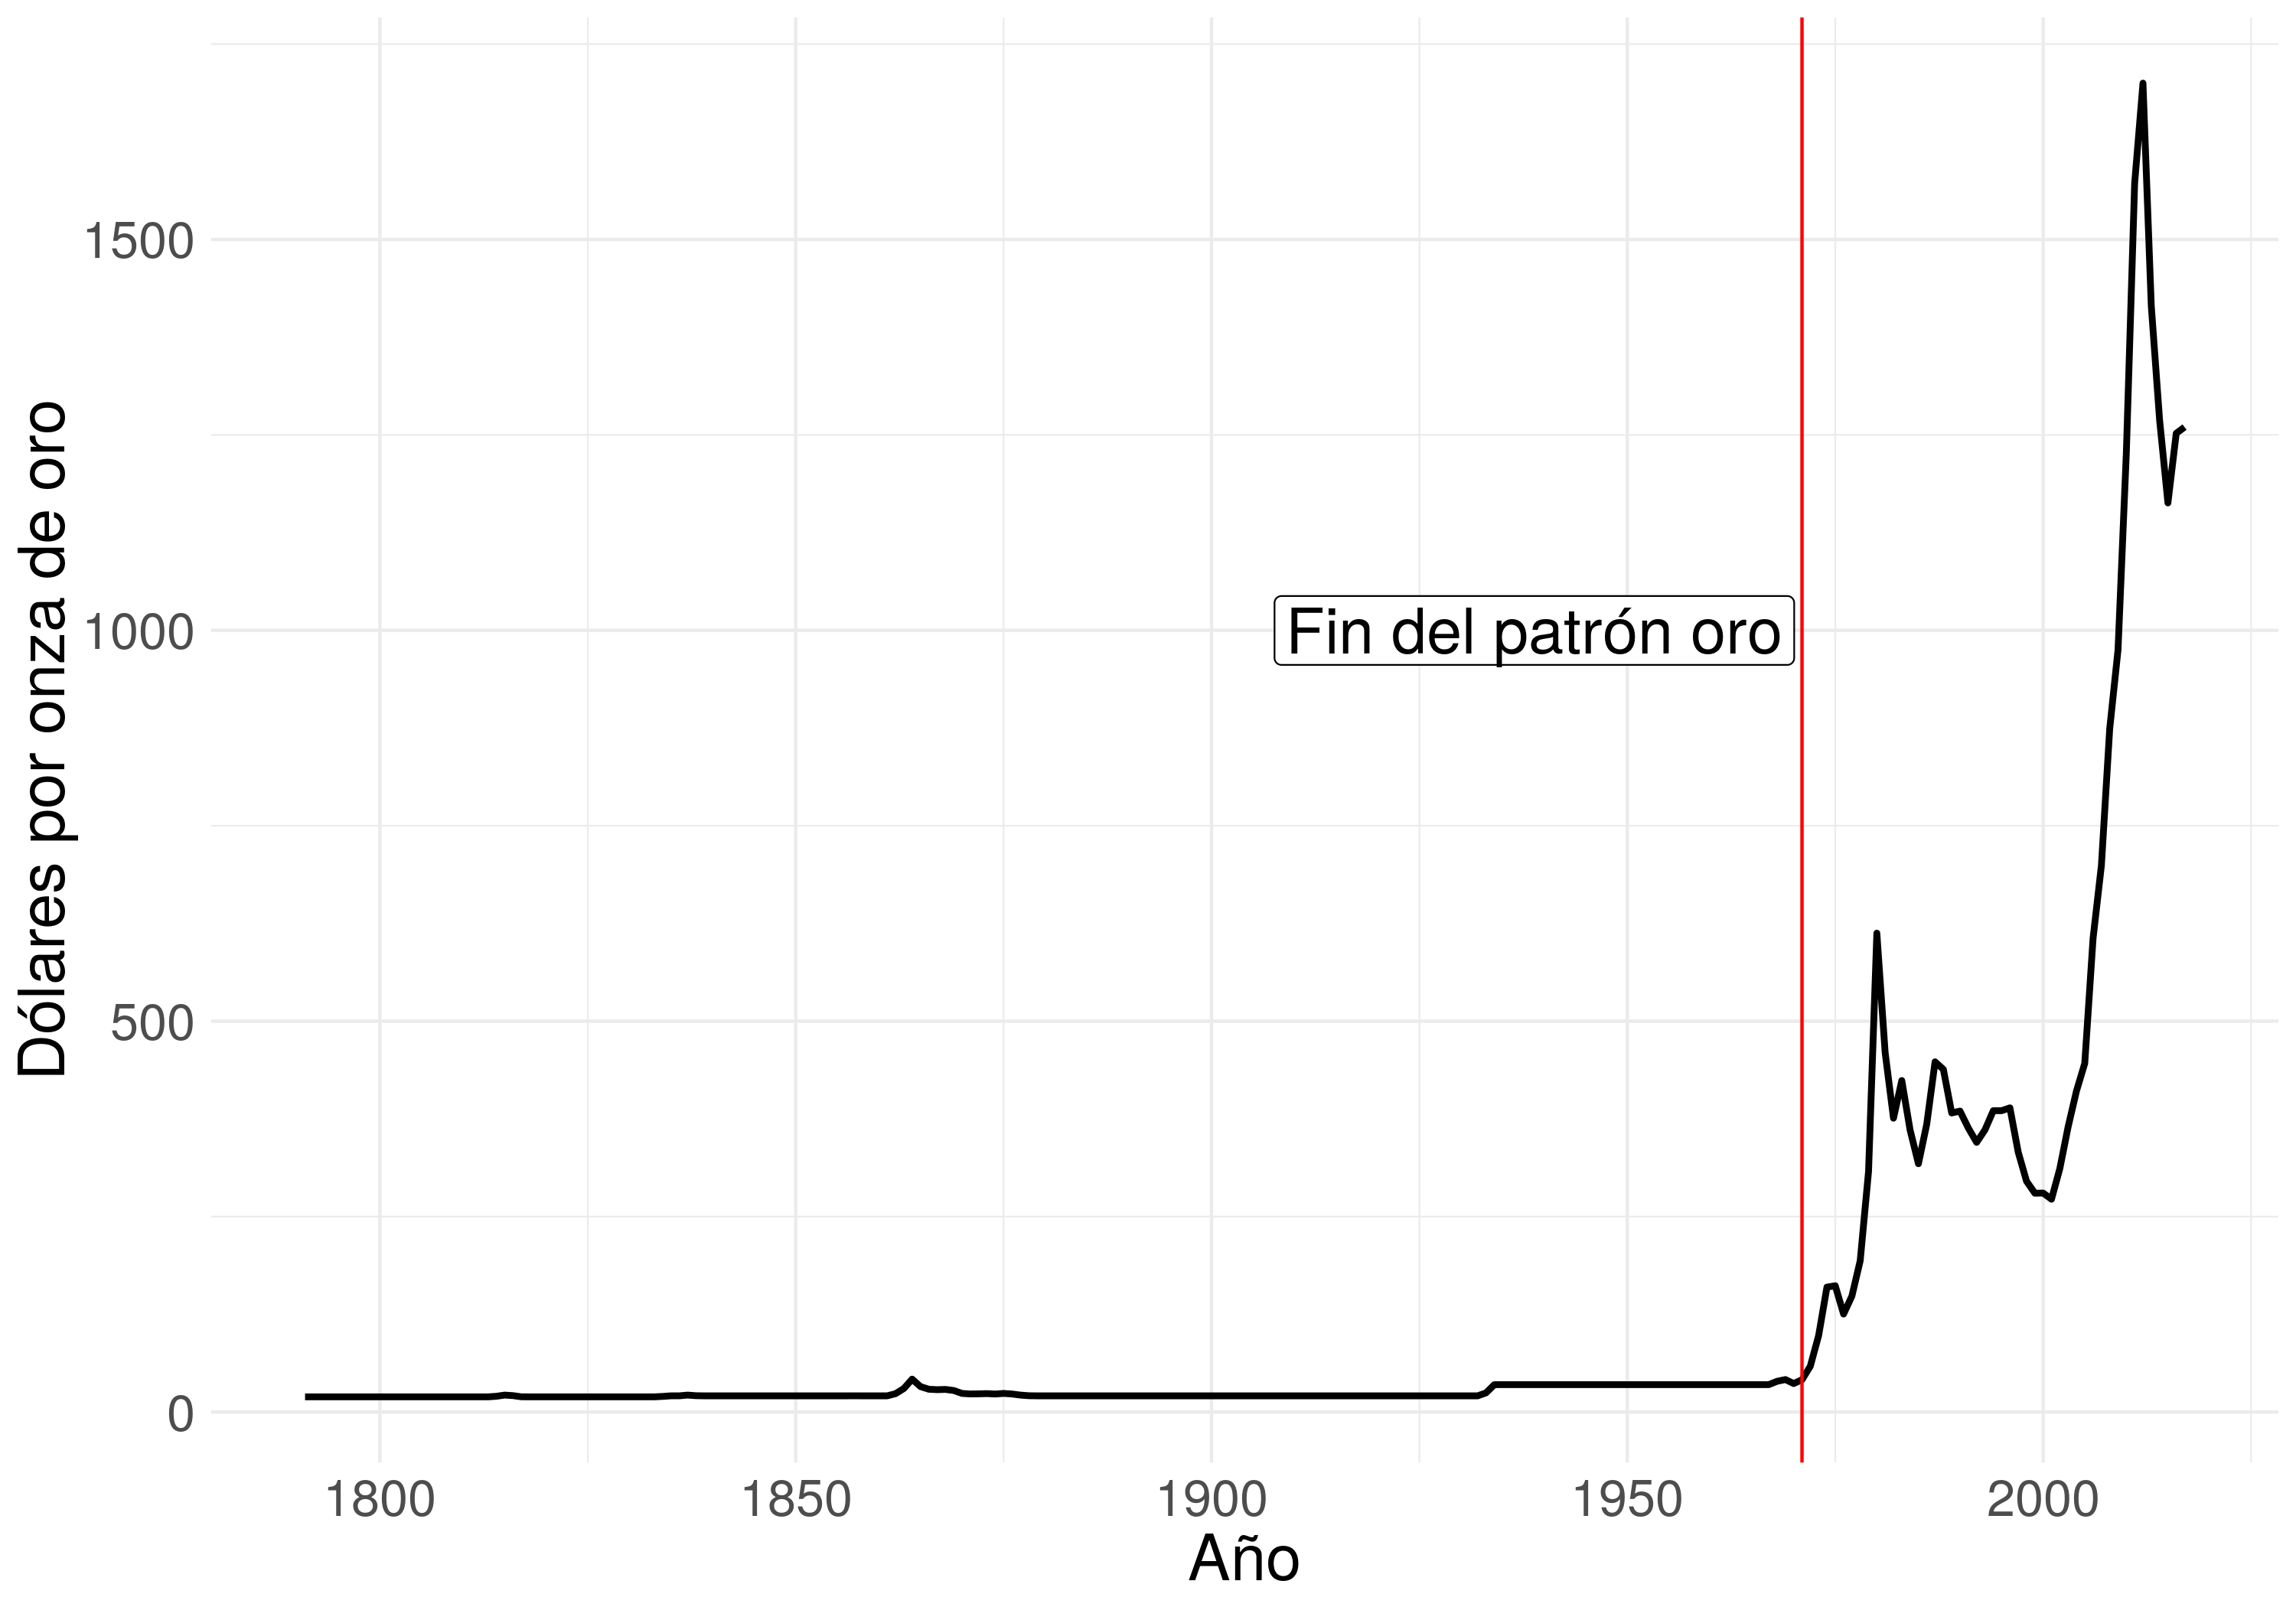
\includegraphics[width=0.8\linewidth]{oro.png}
	\caption{Precios del oro por onza en el mercado de Nueva York} \label{fig:oro}
\end{figure}

Dado que lo que se busca en el presente trabajo es realizar un análisis de largo plazo del ciclo económico, esta perturbación nominal oscurece el fenómeno subyacente que se esta buscando. Es por ello que se opto por normalizar las series del PBI y el salario por el precio del oro. De esta forma las series se leen como el producto y el salario expresado en su capacidad de compra de oro. Una alternativa a esto sería dividir por el Indice de Precios al Consumidor, de forma tal que ambas series se expresen en capacidad de poder adquisitivo constante. 

La decisión de expresar el PBI y el salario en capacidad constante de compra de oro y no poder adquisitivo constante se fundamenta en qué, en tanto el desarrollo de la productividad implica un abaratamiento de la generalidad de las mercancías que componen un indice de precios, y el aumento de la productividad es un fenómeno tendencial de la economía, el PBI expresado en una capacidad de compra constante conserva de forma subyacente una tendencia creciente que oscurece el comportamiento cíclico. El oro, sin embargo, también expresa potencialmente una tendencia al aumento de la productividad en su extracción, no obstante lo cual su precio se encuentra fundamentalmente determinado por el ciclo económico, en tanto constituye un refugio de valor. Este comportamiento contracíclico del precio del oro lo que logra es visibilizar el ciclo en lugar de ocultarlo detrás de una tendencia al aumento de la productividad,y por lo tanto facilita el análisis empírico para el objetivo trazado por el presente trabajo

De acuerdo con lo anterior, la figura \ref{fig:PBI} muestra la serie de el PBI de Estados Unidos entre el 1900 y 2017, expresado en oro. Por su parte la figura \ref{fig:salario} muestra la serie del salario horario de un obrero de la producción en Estados Unidos entre 1900 y 2017, expresado en Oro.

 En ambos casos se resaltan en rojo los períodos de crisis conocidos en la literatura económica, y en líneas punteadas aquellas crisis puntuales que se produjeron en un año particular. La tabla \ref{tabla_crisis} marca el detalle de estas.

\begin{figure}[H]
	\centering
	\subfigure[PBI expresado en Oro]{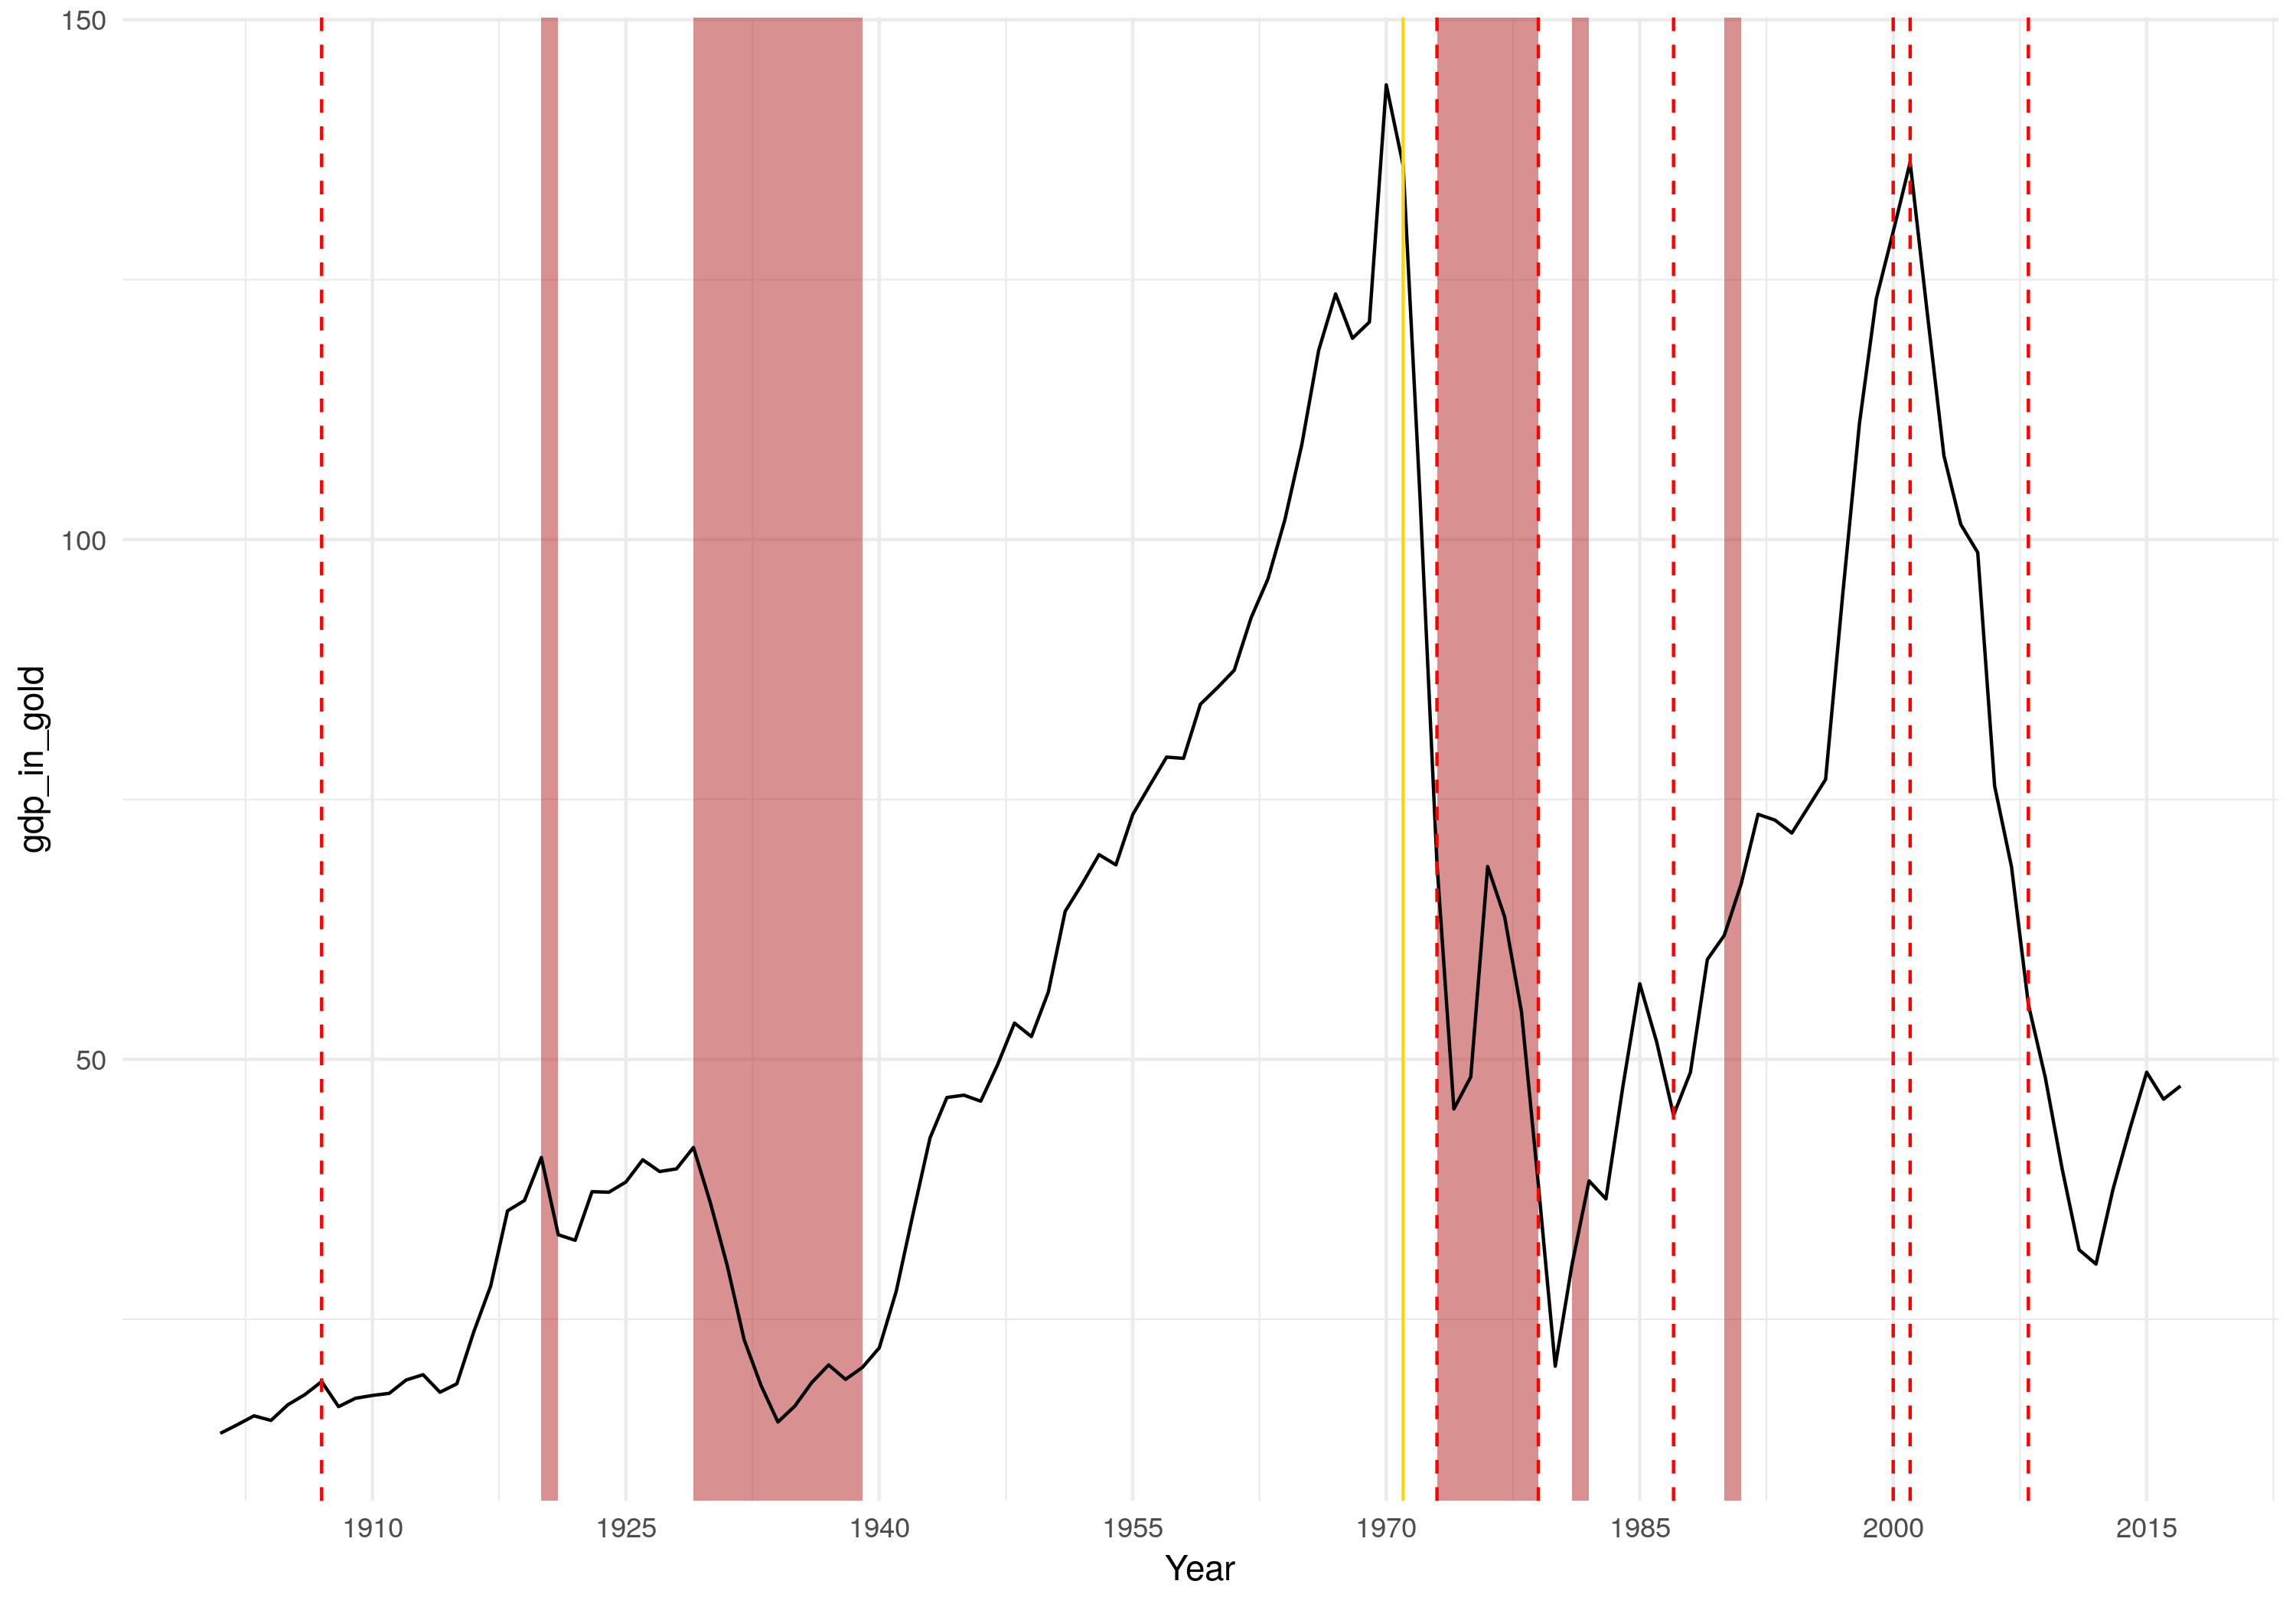
\includegraphics[width=0.75\linewidth]{gdp_in_gold_eda.PNG}
	\label{fig:PBI}}
	\subfigure[Salario expresado en Oro]{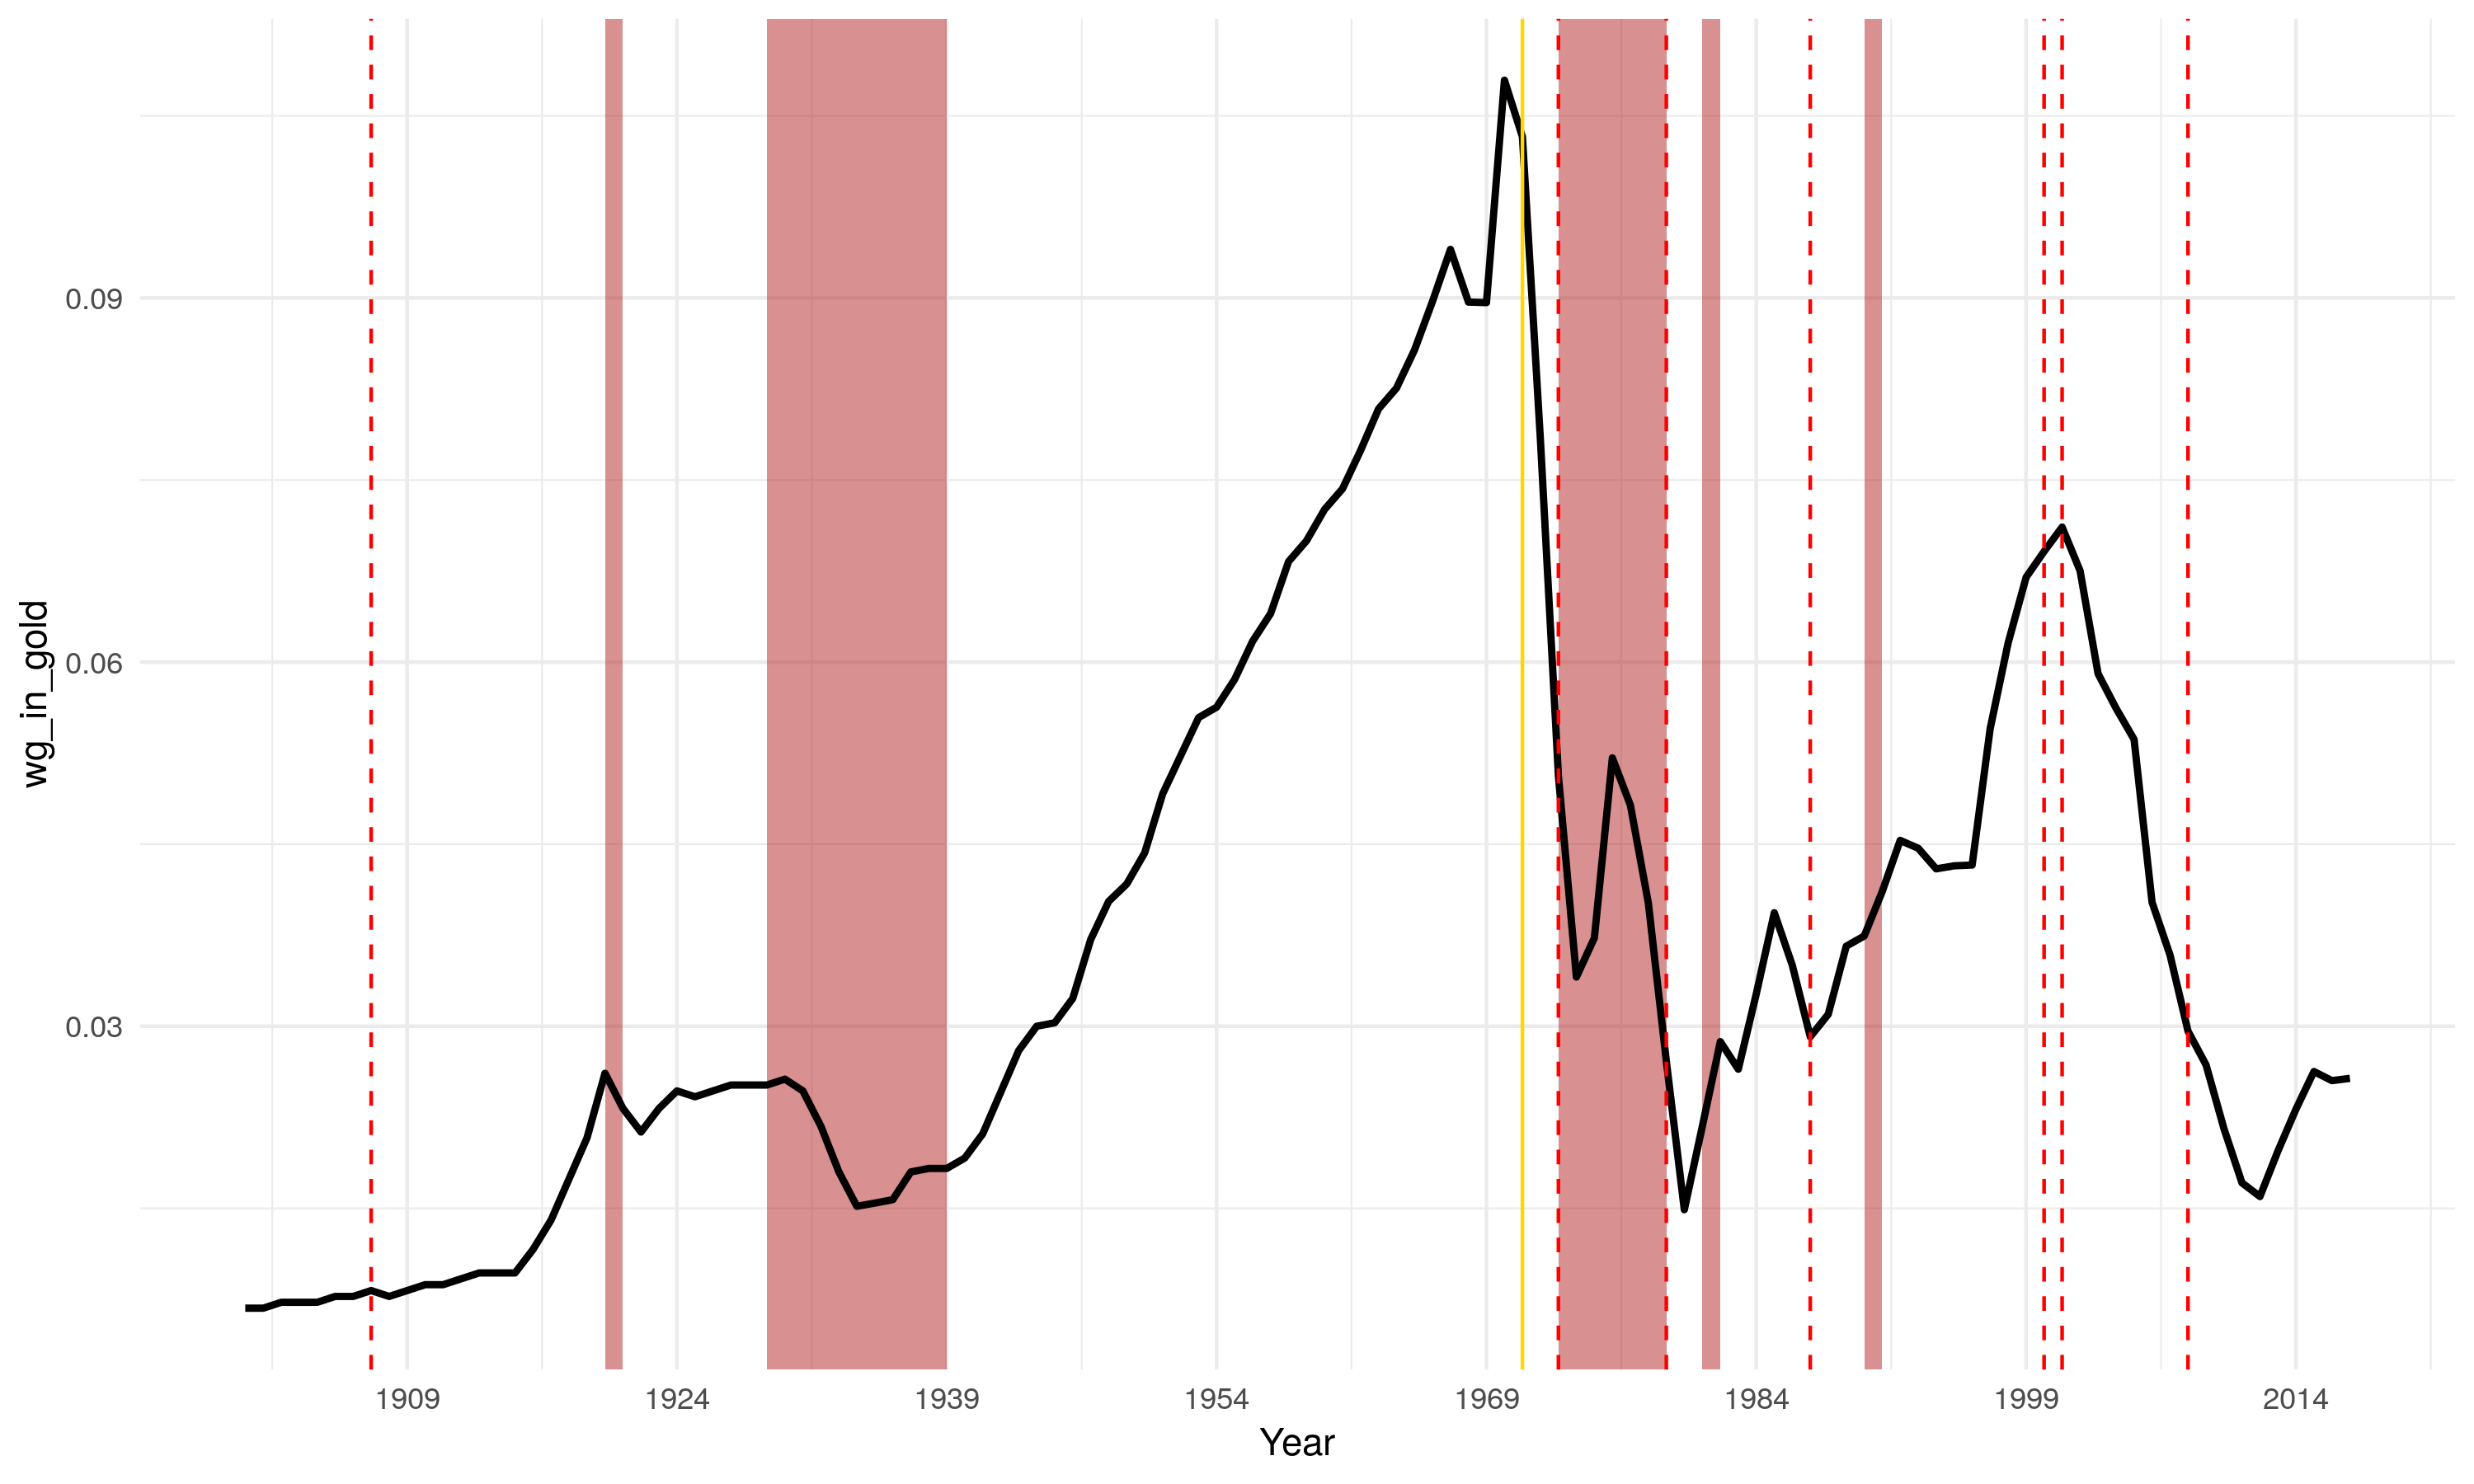
\includegraphics[width=0.75\linewidth]{wg_in_gold_eda.PNG}
	\label{fig:salario}}
	\caption{Series Expresadas en Oro. Destacado de crisis conocidas} \label{fig:series_crisis}
\end{figure}



% latex table generated in R 3.5.1 by xtable 1.8-3 package
% Tue Oct 16 20:07:52 2018
\begin{table}[ht]
	\centering
	\begin{tabular}{ll}
		\hline
		Periodo & Crisis \\ 
		\hline
		1907 & Pánico de 1907 \\ 
		1920 – 1921 & Depresión de 1920 – 21 \\ 
		1929 – 1939 & La gran depresión \\ 
		1970s & 1970s Crisis Energética \\ 
		1973 & Shock de preciso del petróleo de la OPEC(1973) \\ 
		1979 & Revolución Iraní\\ 
		1980s & Recesión de principio de los 80'\\ 
		1987 & Black Monday \\ 
		1990s & Recesión de principio de los 90'\\ 
		2000 & Burbuja de las Dot-com \\ 
		2001 & 911 \\ 
		2008 & Crisis de las subprime \\ 
		\hline
	\end{tabular}
\caption{Principales crisis en EEUU y el mundo. Fuente: Instituto Caproasia}
\label{tabla_crisis}
\end{table}




En primer lugar lo que se observa es la similitud de ambas series, en términos generales. Ambas muestran tres picos, durante los 20', en 1970 y el 2000, seguidos de caídas profundas. La normalización por el precio del oro permite ver un gran ciclo con tres oscilaciones, por lo menos de manera aparente, durante el siglo XX. Las crisis revisadas por la literatura de historia económica parecen tener su correlato en los movimientos observados en ambas series. Por su parte, también es interesante resaltar que el tercer movimiento ascendente, cuyo punto álgido se encuentra en el año 2000, lleva a un valor similar al del movimiento oscilatorio previo para el caso del PBI, pero no para el salario. Esto expresa que la distribución del PBI en salario y ganancia se modificó en el último período. 

%%%%%%%%%%%%%%%%%%%%%%%%%%%%%%%%%%%%%%%%%%%%%%%%%%%%%%%%%%%%%%%%%
\section{Análisis de ciclos de baja frecuencia en series de tiempo de variables macroeconómicas}
\subsection{Tasa de interés de largo plazo}

En el siguiente apartado se analizan los ciclos que se pueden detectar en la serie de tasas de interés de largo plazo de los bonos del Tesoro de los EE.UU.

En la figura \ref{fig:ir_orig} se puede observar la serie de tasas de interés de largo plazo por año. En la misma se puede observar una diferencia significativa en el nivel de tasas de la segunda mitad del siglo XX respecto de los años anteriores, sobre todo posteriores a 1970. Esto corresponde a niveles altos de inflación en los EE.UU. en este periodo y la siguiente paulatina baja de la inflación llegando al siglo XXI.

\begin{figure}[H]
	\centering
	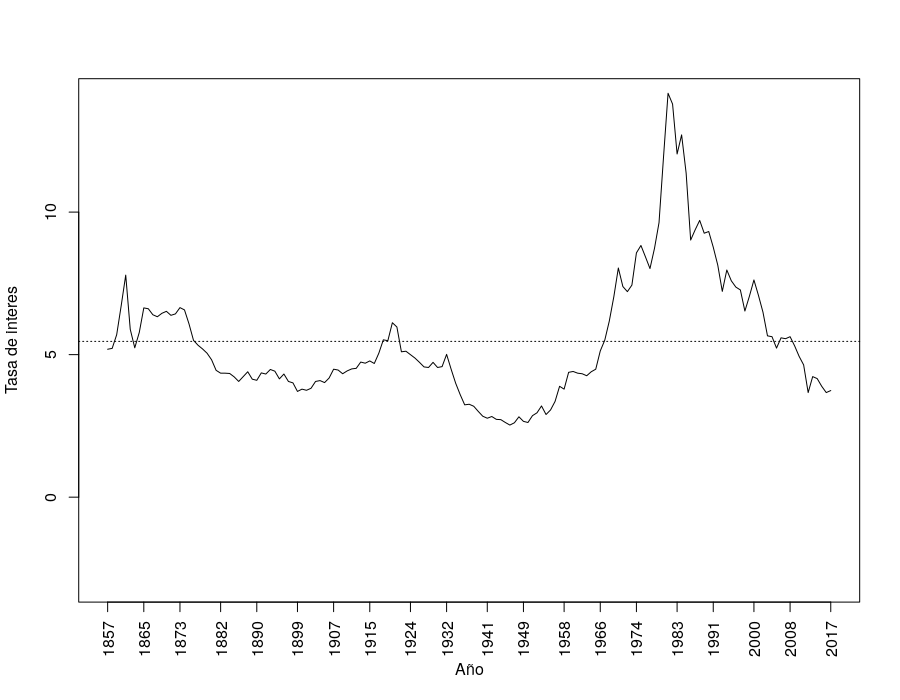
\includegraphics[width=0.75\linewidth]{ir_orig.png}
	
	\caption{Tasa de interés de largo plazo de los EE.UU.}
	\label{fig:ir_orig}
\end{figure}

A continuación (Figura \ref{fig:ir_diff_acf}) se muestran el gráficos de diferencias (cambios absolutos, en puntos porcentuales, de la tasa de interés de largo plazo, por año) y la autocorrelación de las diferencias. Se observa que hay una leve correlación con el periodo siguiente al lag 0, pero en general la autocorrelación es muy similar a un random walk.

\begin{figure}[H]
	\centering
	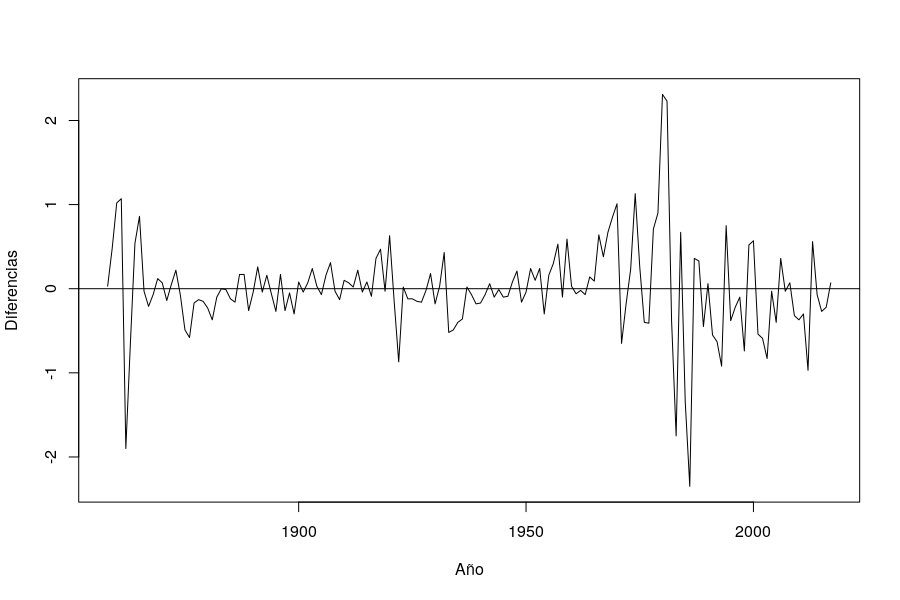
\includegraphics[width=0.75\linewidth]{ir_diff.png}
	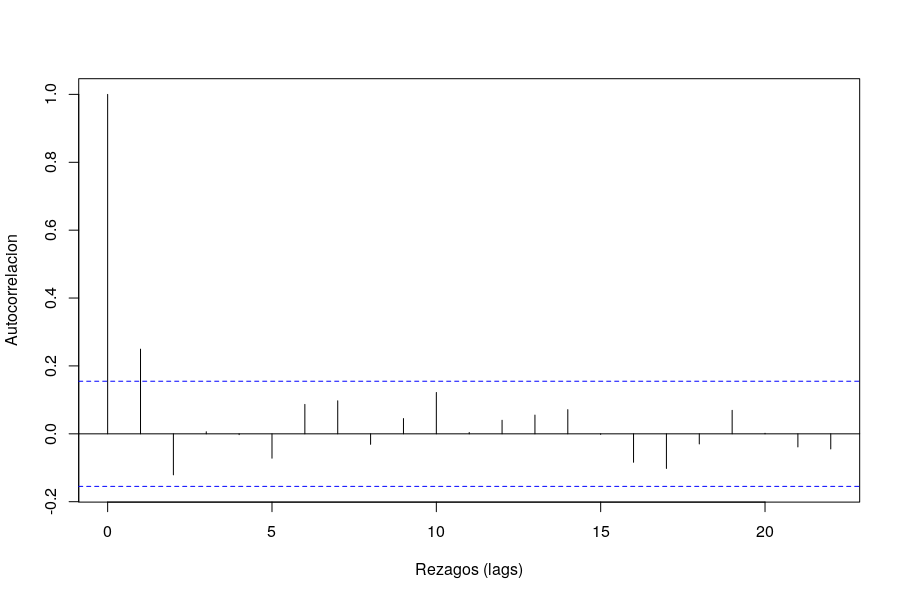
\includegraphics[width=0.75\linewidth]{ir_diff_acf.png}
	\caption{Diferencias (arriba) y autocorrelación de las diferencias (abajo) de las tasas de interes.} 	
	\label{fig:ir_diff_acf}
\end{figure}

Si bien no se observan tendencias de largo plazo en las diferencias y estas sirven habitualmente para centrar las series, la diferenciación sólo captura las frecuencias más altas, dejando de lado las de largo plazo, por lo que con este análisis sólo se pueden investigar ciclos de corta duración. Para poder investigar ciclos de mayor duración se investiga la transformada de Fourier de la serie, que permite observar las frecuencias y amplitudes que componen la serie. En la figura \ref{fig:ir_fft} puede observarse el espectro de frecuencias de la serie de tasas de interés centrada en su media.

\begin{figure}[H]
	\centering
	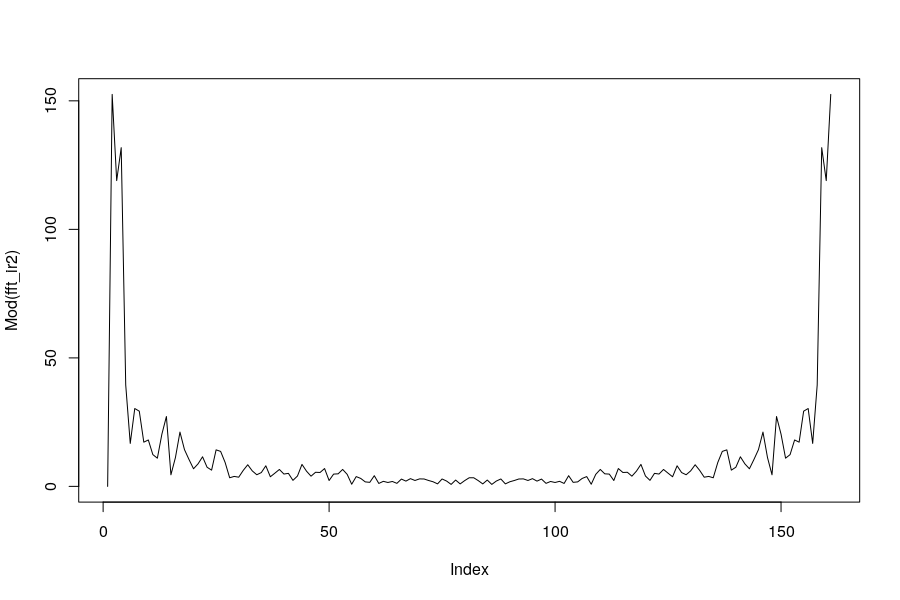
\includegraphics[width=0.8\linewidth]{ir_fft.png}
	\caption{Transformada de Fourier de la tasa de interés} 	
	\label{fig:ir_fft}
\end{figure}

Se observa que hay frecuencias bajas con gran amplitud. Si descomponemos la serie por las frecuencias más bajas, se puede observar la serie en rojo de la figura \ref{fig:ir_orig_resid} que resulta de la descomposición de la serie original por las frecuencias más bajas. Puede observarse que la serie aún presenta autocorrelación (en detalle la autocorrelación de la figura \ref{fig:ir_resid_acf})

\begin{figure}[H]
	\centering
	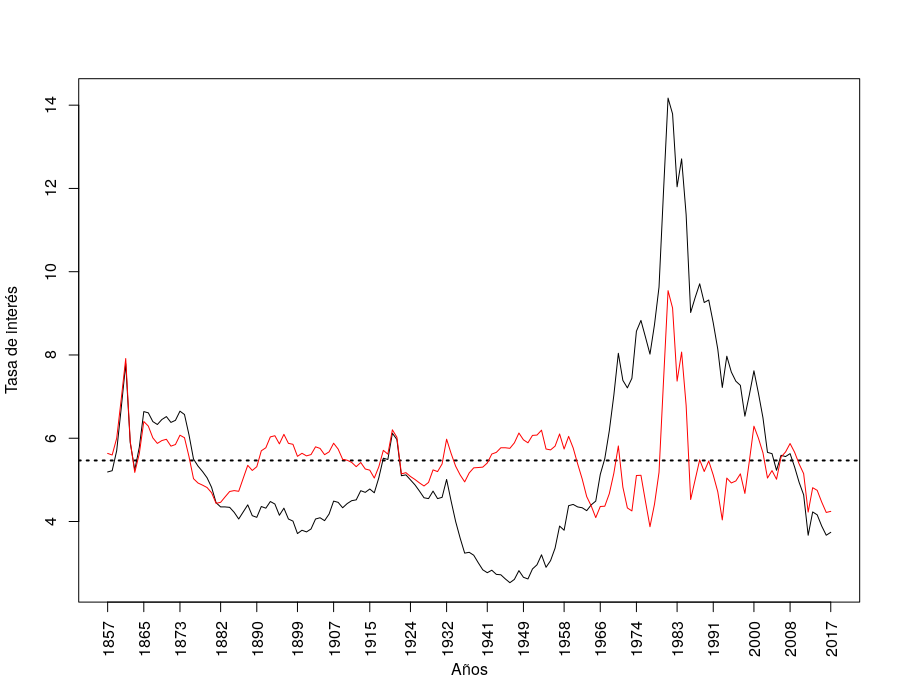
\includegraphics[width=0.8\linewidth]{ir_orig_resid.png}
	\caption{Serie original y residuos (en rojo) de descomponer por las frecuencias más bajas} 	
	\label{fig:ir_orig_resid}
\end{figure}

\begin{figure}[H]
	\centering
	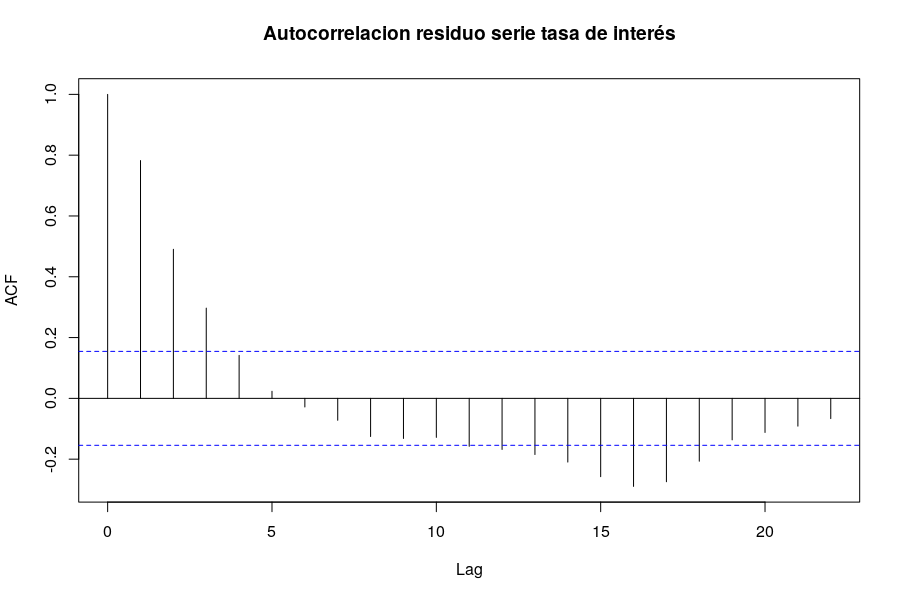
\includegraphics[width=0.8\linewidth]{ir_resid_acf.png}
	\caption{Autocorrelación de la parte no explicada por la descomposición de las frecuencias más bajas} 	
	\label{fig:ir_resid_acf}
\end{figure}

\subsection{Índice de precios al consumidor}
La serie de nivel de precios al consumidor(\textit{"Consumer Price Index"}, Índice de precios al consumidor, \textit{CPI} por sus siglas en inglés, \textit{IPC} en español) de los EE.UU. está expresada en base 100, con base en el promedio anual de 1982-1984. La serie de tiempo original se puede observar en la figura \ref{fig:cpi_orig}, donde se observa el fenómeno exponencial de la inflación a través de los años. Asimismo, se puede observar una diferencia entre los siglos XIX y XX, especialmente tras el rompimiento con el sistema de patrón oro de 1971 durante la administración Nixon y los años previos al abandono de este sistema de respaldo de papel moneda.

\begin{figure}[H]
	\centering
	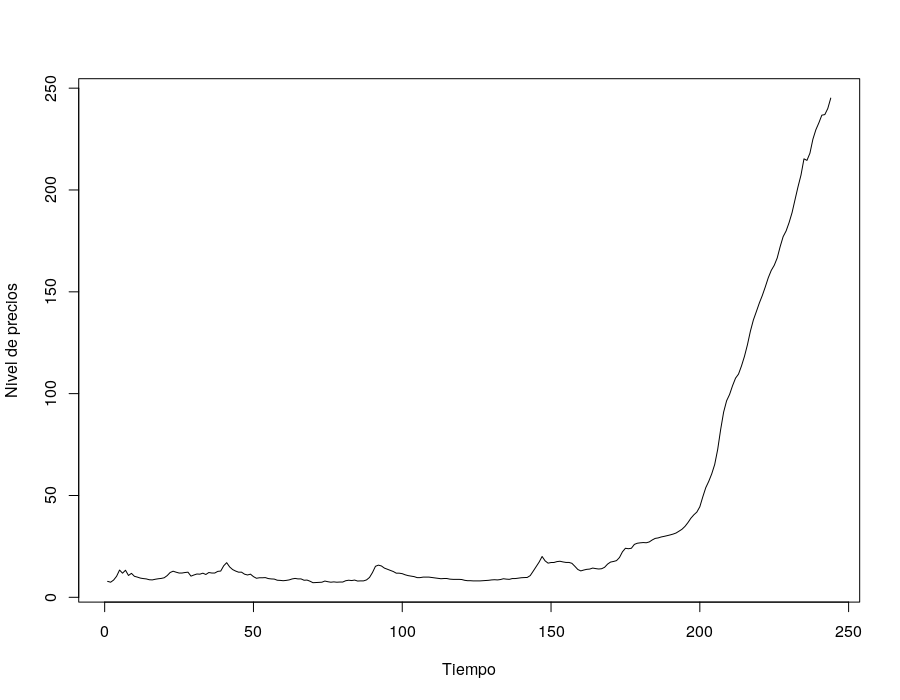
\includegraphics[width=0.8\linewidth]{cpi_orig.png}
	\caption{Índice de precios al consumidor en los EE.UU., base: promedio anual de 1982-1984} 	
	\label{fig:cpi_orig}
\end{figure}


Este hecho de diferencias seculares en el nivel de precios puede observarse con mayor detalle en la figura \ref{fig:cpi_log10_tend} donde se observa el logaritmo en base diez de los datos originales con tendencias lineales calculadas para los años previos y posteriores a 1900, apreciandose el cambio de tendencia del crecimiento del nivel de precios. En este último gráfico se han marcado también con líneas punteadas rojas acontecimientos notables de la historia de los EE.UU. y mundiales para tomar como referencia en los cambios de estas variables macroeconómicas.


\begin{figure}[H]
	\centering
	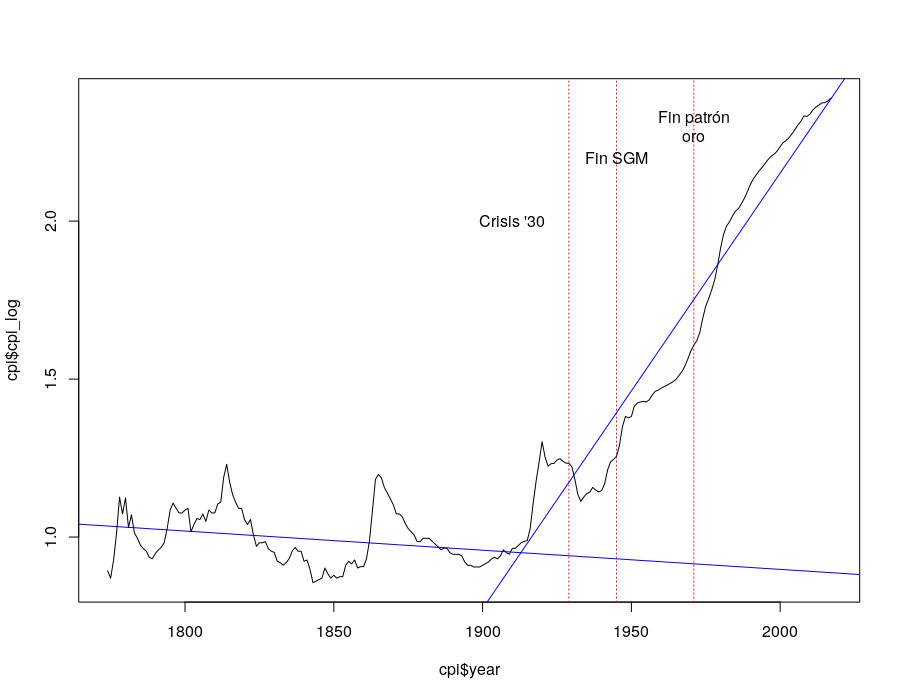
\includegraphics[width=0.8\linewidth]{cpi_log10_tend.png}
	\caption{Log 10 y tendencias ajustadas antes y después del año 1900} 	
	\label{fig:cpi_log10_tend}
\end{figure}

Se elige centrar la serie de precios por las tendencias lineales para poder evitar que se distorsione el ciclo usando técnicas que ajusten mejor a datos no lineales, debido a que se analizarán los residuos de estas series con transformaciones de Fourier en busca de poder explicarlos y de buscar la existencia de ciclos alrededor de estas tendencias. Se pueden observar las tendencias centradas y la alternancia alrededor de cero en la figura \ref{fig:cpi_log10_cntr}.

\begin{figure}[H]
	\centering
    \subfigure{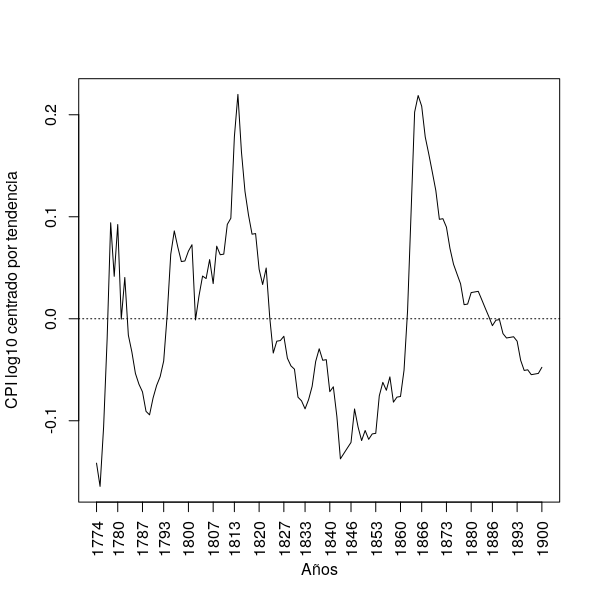
\includegraphics[width=0.49\linewidth]{cpi_log10_cntr_pre.png}}
	\subfigure{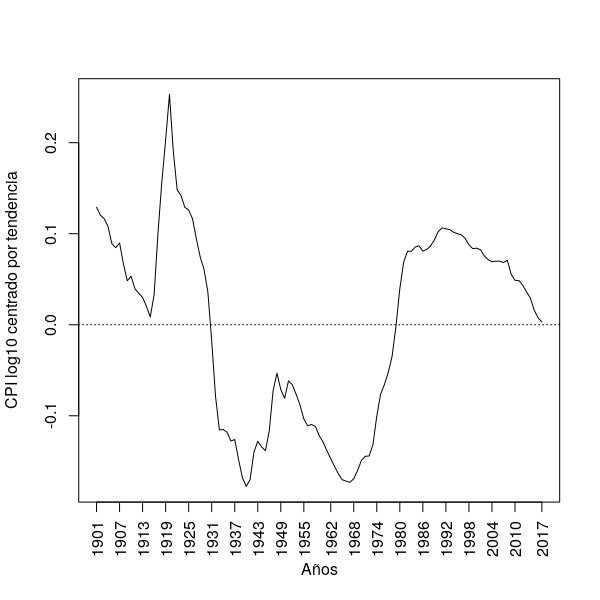
\includegraphics[width=0.49\linewidth]{cpi_log10_cntr_post.png}}
	\caption{IPC log10 centrado por tendencia lineal antes (izquierda) y después (derecha) de 1900} 	
	\label{fig:cpi_log10_cntr}
\end{figure}

Pasamos ahora al análisis de los residuos: la serie centrada por las tendencias. Realizamos las transformadas de Fourier sobre estas nuevas series. El resultado puede observarse en la figura \ref{fig:cpi_log10_cntr_fft}, en la que puede verse que las frecuencias más bajas son las que cuentan con mayor amplitud.

\begin{figure}[H]
	\centering
    \subfigure{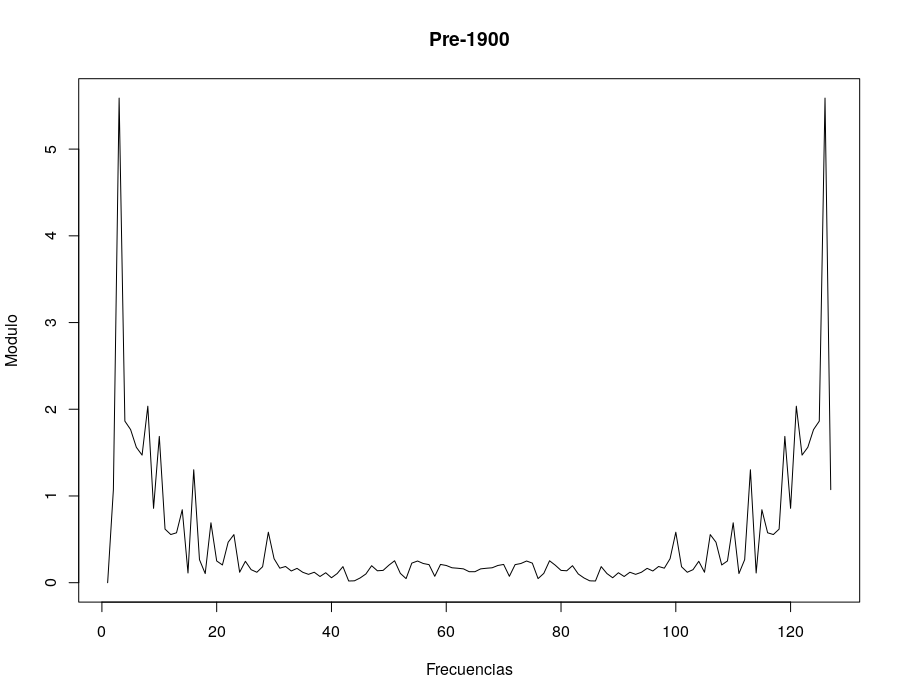
\includegraphics[width=0.49\linewidth]{cpi_fft_pre1900.png}	}
	\subfigure{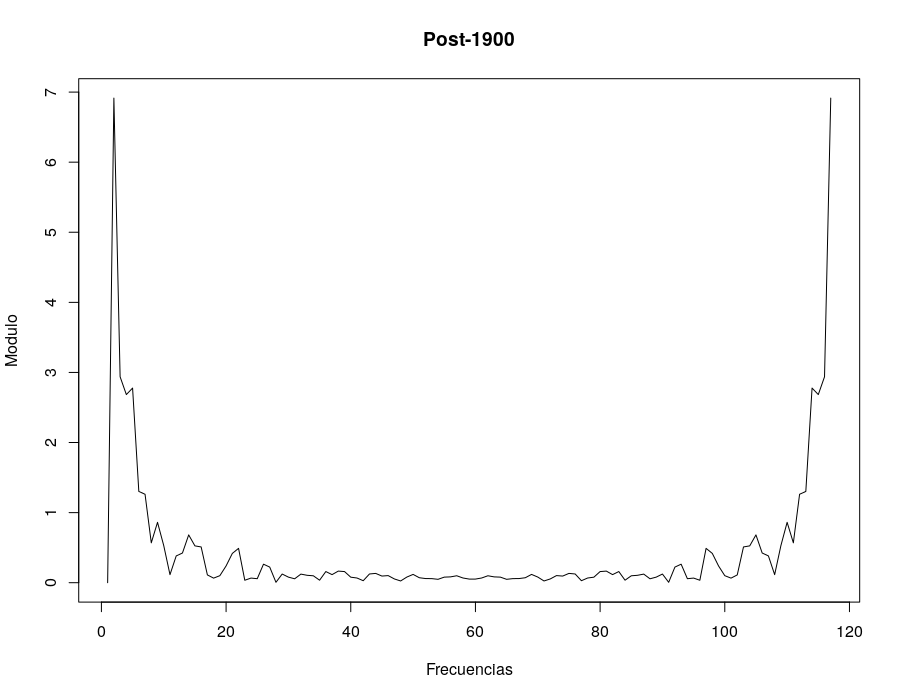
\includegraphics[width=0.49\linewidth]{cpi_fft_post1900.png}}
	\caption{IPC log10 centrado por tendencia lineal antes (izquierda) y después (derecha) de 1900} 	
	\label{fig:cpi_log10_cntr_fft}
\end{figure}

Ahora podemos tomar las frecuencias más bajas y descomponer la serie centrada por ellas, analizar el ajuste de estas nuevas series y visualizar la serie resultante de esta descomposición. En la figura \ref{fig:cpi_cntr_antifft} se pueden observar las primeras 9 componentes de más baja frecuencia de la transformada de Fourier y, en azul, el residuo de restar los valores de la transformación de la serie de tiempo. En la figura \ref{fig:cpi_cntr_acf} puede observarse también que aún puede continuar explicándose los residuos en azul debido a que hay rezagos que tienen correlación entre sí. Esto demuestra que, si bien existen ciclos de bajas frecuencias pueden descomponerse series de más altas frecuencias que corresponderían a ciclos de medio y corto plazo.

\begin{figure}[H]
	\centering
    \subfigure{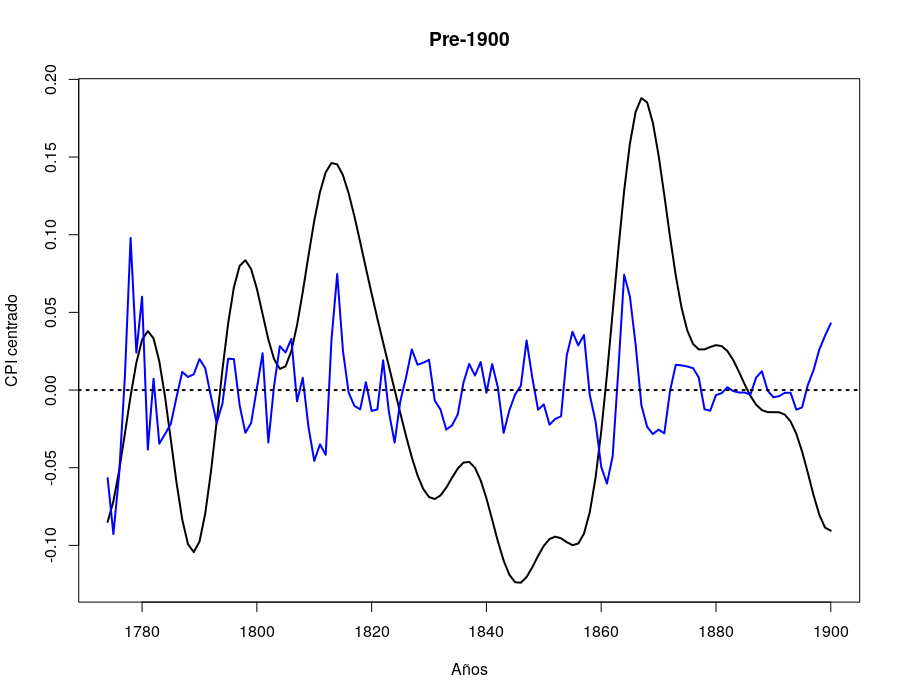
\includegraphics[width=0.49\linewidth]{cpi_antifft_pre1900.png}}
	\subfigure{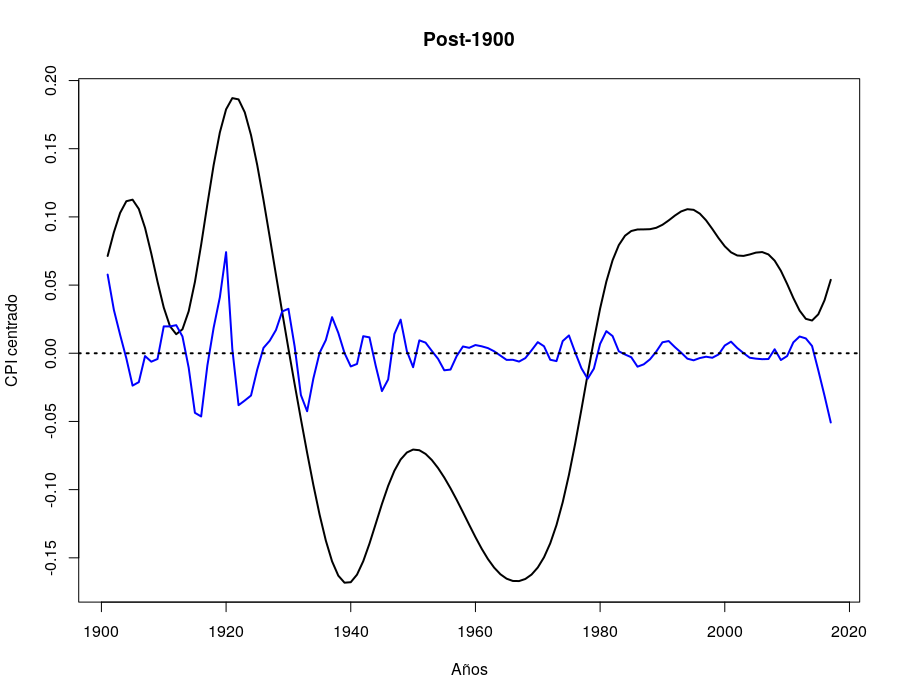
\includegraphics[width=0.49\linewidth]{cpi_antifft_post1900.png}}
	\caption{Residuos (en azul) luego de quitar las bajas frecuencias} 	
	\label{fig:cpi_cntr_antifft}
\end{figure}

\begin{figure}[H]
	\centering
    \subfigure{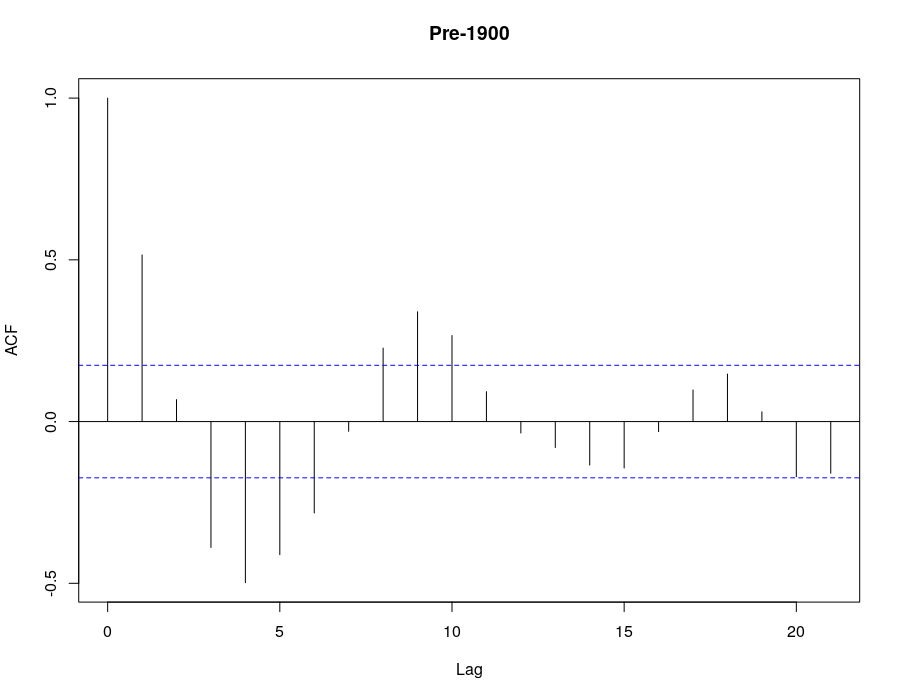
\includegraphics[width=0.49\linewidth]{cpi_acf_pre1900.png}}
	\subfigure{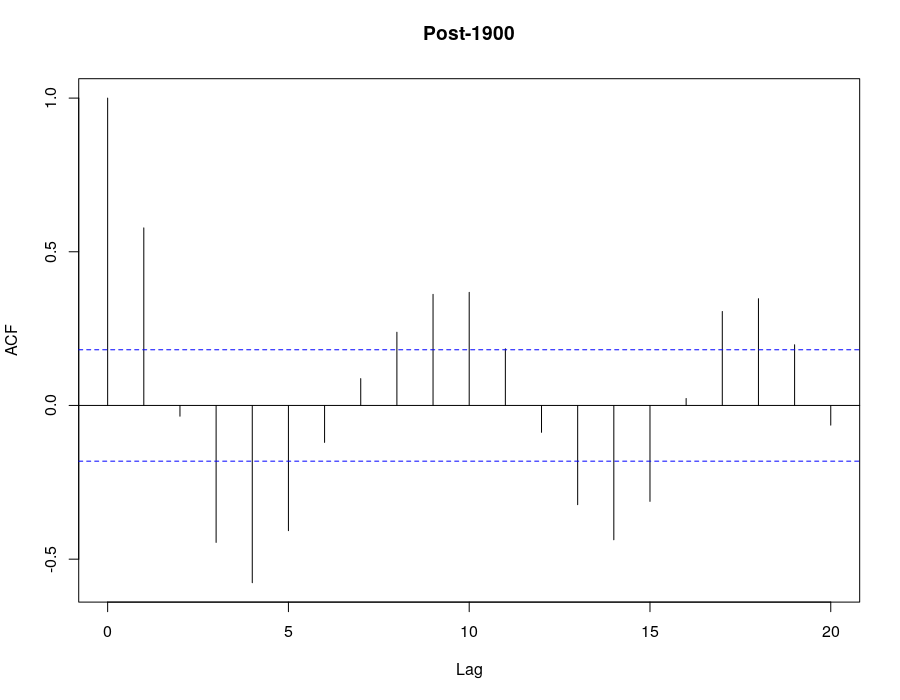
\includegraphics[width=0.49\linewidth]{cpi_acf_post1900.png}}
	\caption{Autocorrelación de los residuos}
	\label{fig:cpi_cntr_acf}
\end{figure}

\subsection{PBI real}
Estados Unidos se ha convertido en la economía más poderosa del mundo con el transcurrir de los años desde su independencia por diversos factores. Más allá de las crisis y eventos significativos como pueden ser las guerras mundiales, la Guerra Fría, el abandono del patrón oro y un sinfín de políticas económicas de diverso tenor, uno de los efectos más notables es la forma en que sostiene un crecimiento de muy largo plazo casi constante a lo largo de su historia reciente. Esto se puede visualizar en la figura \ref{fig:PBI_orig} en donde, a la izquierda se puede visualizar el PBI real de los EE.UU. y a la derecha, el logaritmo en base 10 de la serie de la izquierda en donde además se ajustó una linea mediante mínimos cuadrados (regresión lineal) ilustrando la tendencia. El ajuste es muy bueno, con un R cuadrado de 99.54\%, lo que demuestra que casi se mantiene constante la tasa de crecimiento a lo largo de todo el periodo considerado en la serie.

\begin{figure}[H]
	\centering
    \subfigure{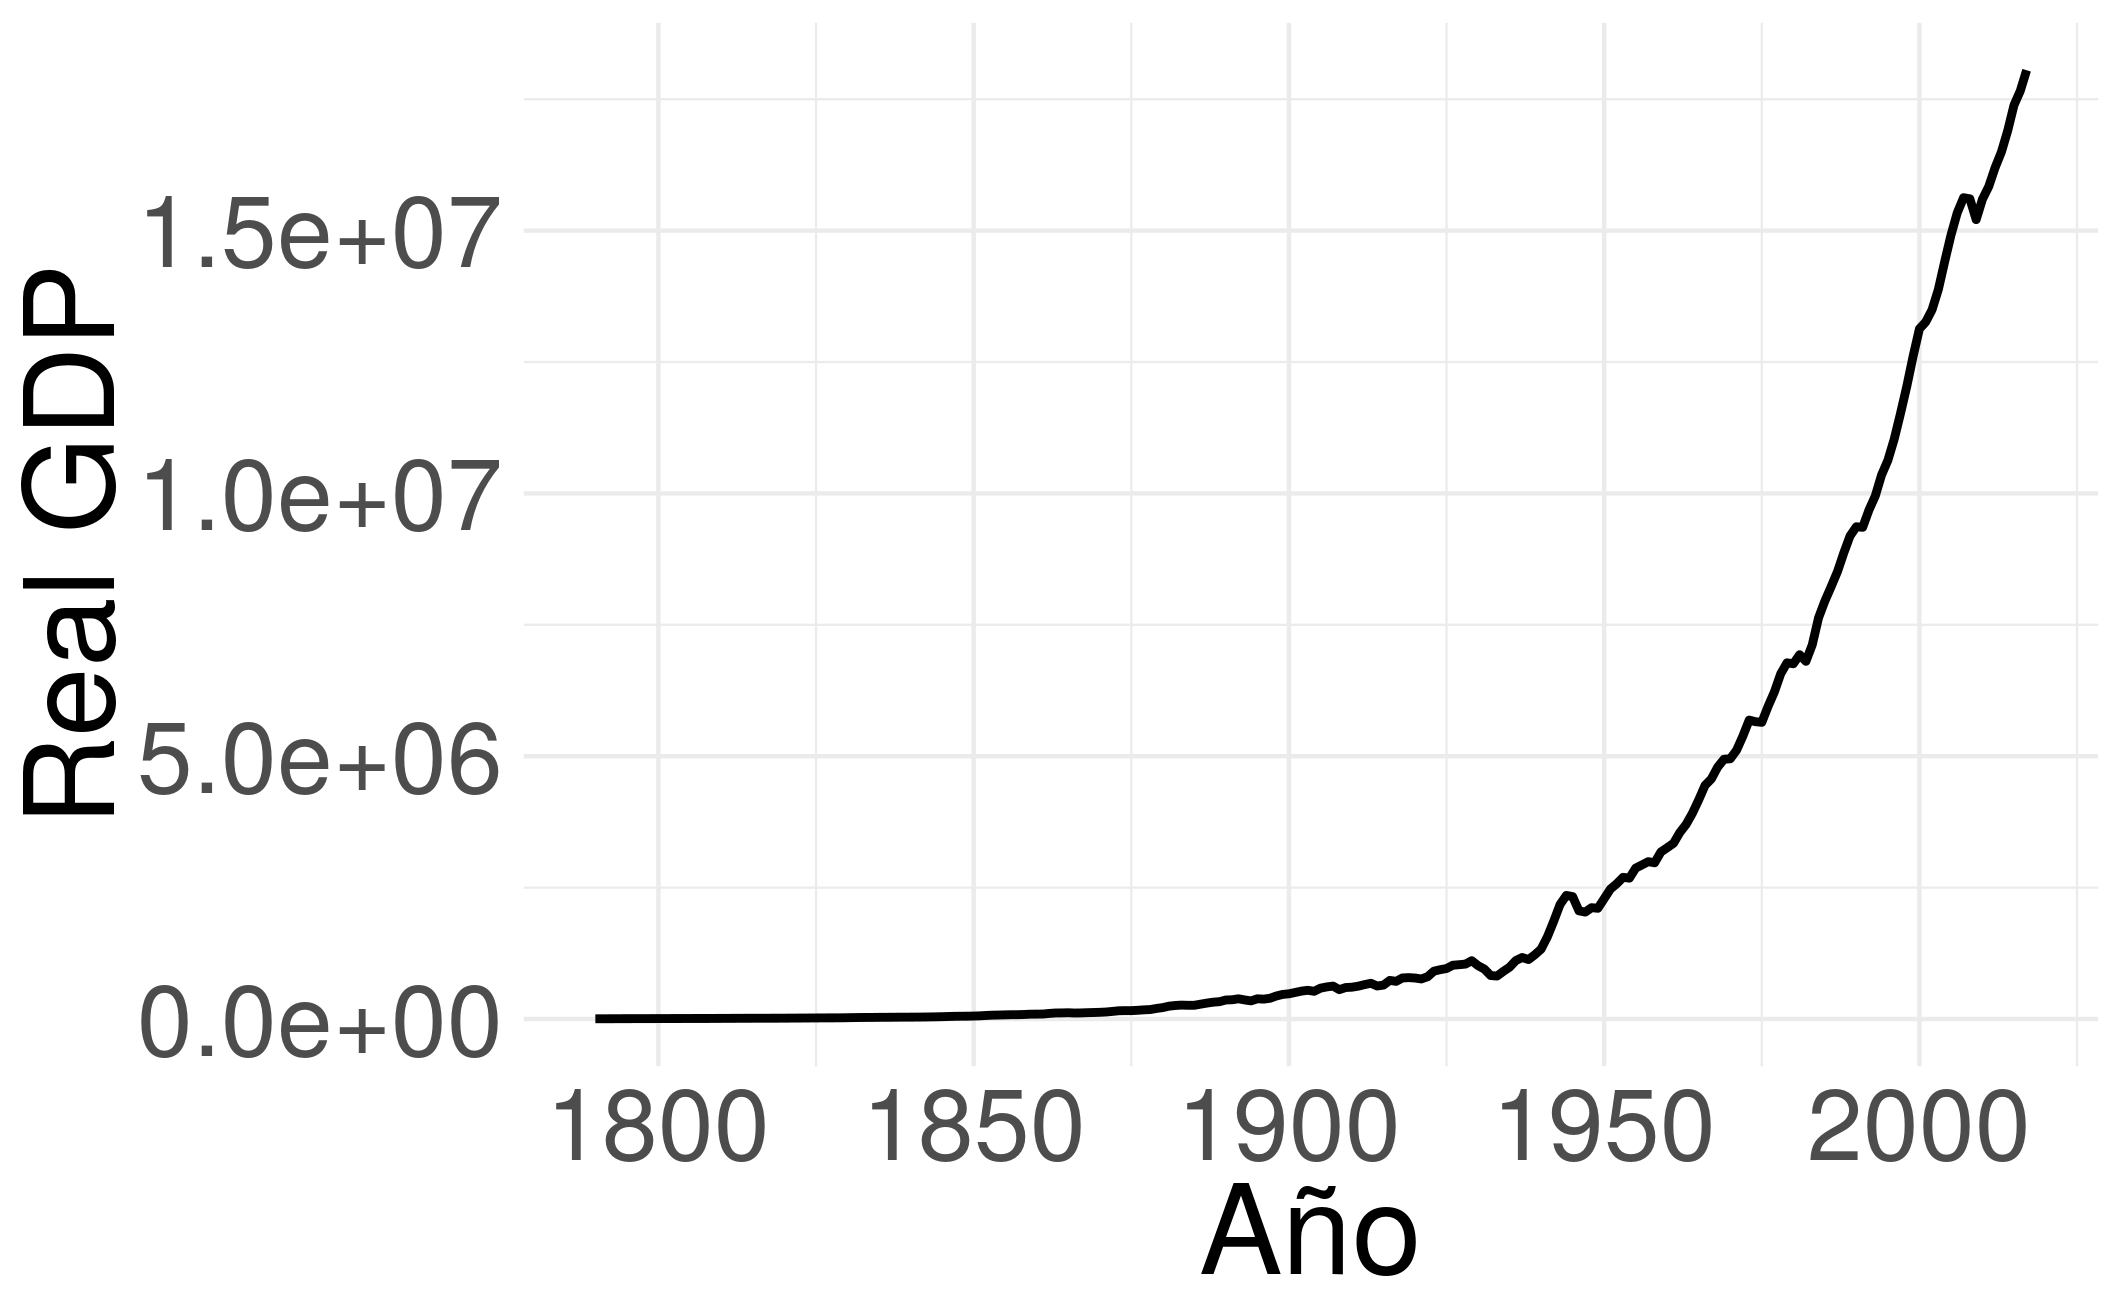
\includegraphics[width=0.49\linewidth]{PBI.png}	}
	\subfigure{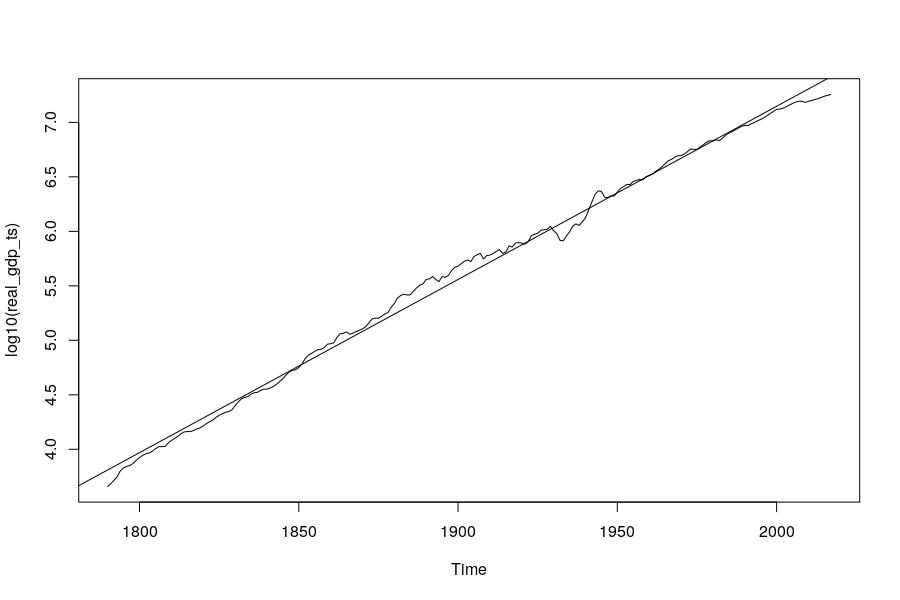
\includegraphics[width=0.49\linewidth]{PBI_log_tend.png}}
	\caption{PBI real (izquierda) y logaritmo en base 10 del PBI real (derecha)} 	
	\label{fig:PBI_orig}
\end{figure}

A pesar de lo enormemente explicativa que es la tendencia lineal sobre el logaritmo de la serie, hay zonas en las que el residuo es estrictamente positivo o negativo, por lo que puede analizarse si hay ciclos en estos residiuos, es decir, alrededor de la tendencia lineal. Los residuos pueden visualizarse en la figura \ref{fig:PBI_cntr}.

\begin{figure}[H]
	\centering
    \subfigure{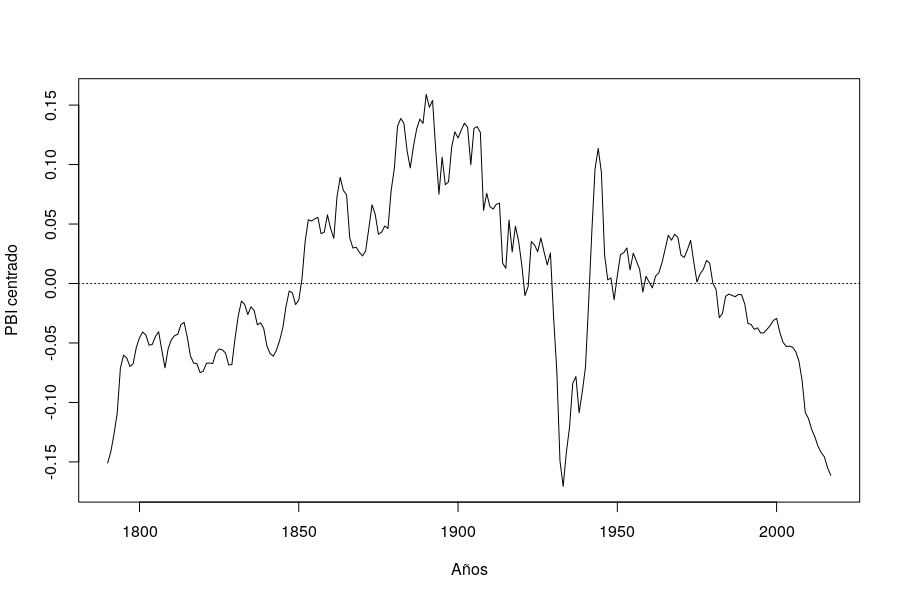
\includegraphics[width=0.8\linewidth]{PBI_centrado.png}}
	\caption{PBI centrado por la tendencia lineal} 	
	\label{fig:PBI_cntr}
\end{figure}


Nuevamente, aplicamos la transformada de Fourier sobre los residuos. Puede observarse el módulo de los vectores formados con respecto a la frecuencia en la figura \ref{fig:PBI_cntr_fft}.

\begin{figure}[H]
	\centering
    \subfigure{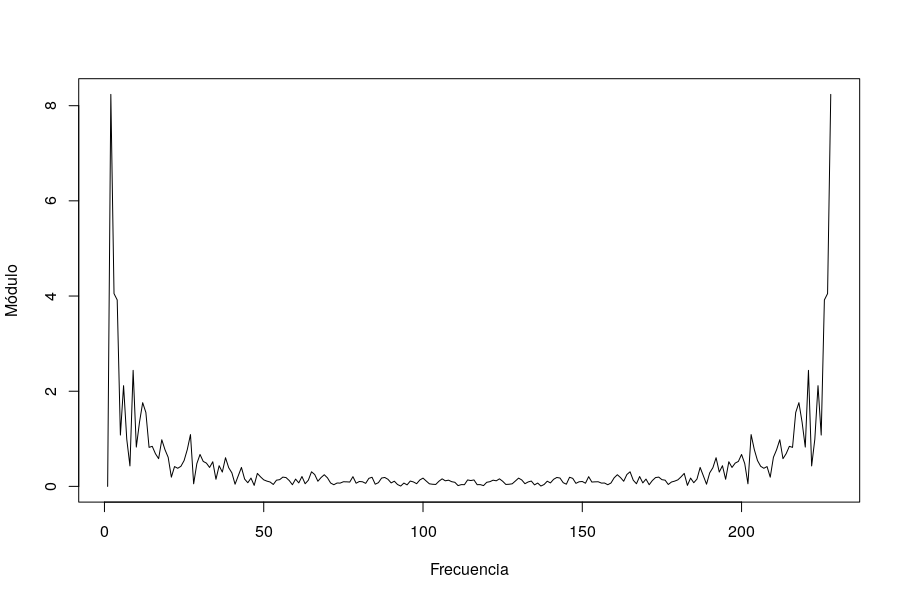
\includegraphics[width=0.8\linewidth]{PBI_centrado_fft.png}}
	\caption{Transformada de Fourier del PBI centrado} 	
	\label{fig:PBI_cntr_fft}
\end{figure}

Luego podemos observar el ajuste de la transformada de Fourier a los datos. Para ello graficamos nuevamente los residuos y la anti-transformada de las frecuencias más bajas de la transformada de Fourier expuesta previamente. Esto se puede observar en \ref{fig:PBI_cntr_antifft}

\begin{figure}[H]
	\centering
    \subfigure{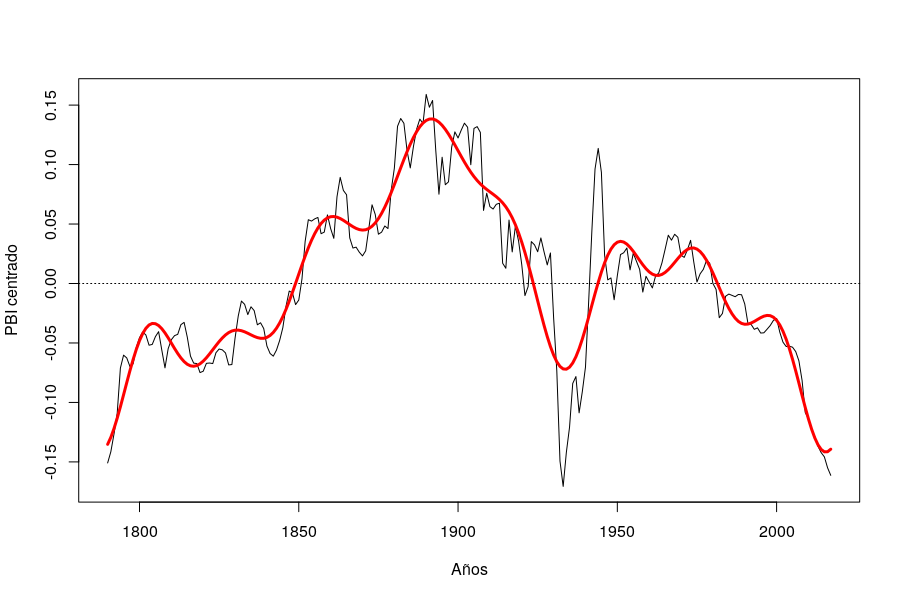
\includegraphics[width=0.8\linewidth]{PBI_centrado_antifft.png}}
	\caption{Serie original y antitransformada de las frecuencias más bajas} 
	\label{fig:PBI_cntr_antifft}
\end{figure}

Nuevamente observamos los residuos explicados de la serie y la autocorrelación de esos residuos en \ref{fig:PBI_fft_resid}. Puede observarse que aún queda estructura por explicar en los residuos dado por ciclos de más baja frecuencia. Esto demuestra que se puede descomponer la serie en ciclos de baja y alta frecuencia, si bien en este estudio estamos mayormente interesados en ciclos de largo plazo (señales de baja frecuencia y alta amplitud).

\begin{figure}[H]
	\centering
    \subfigure{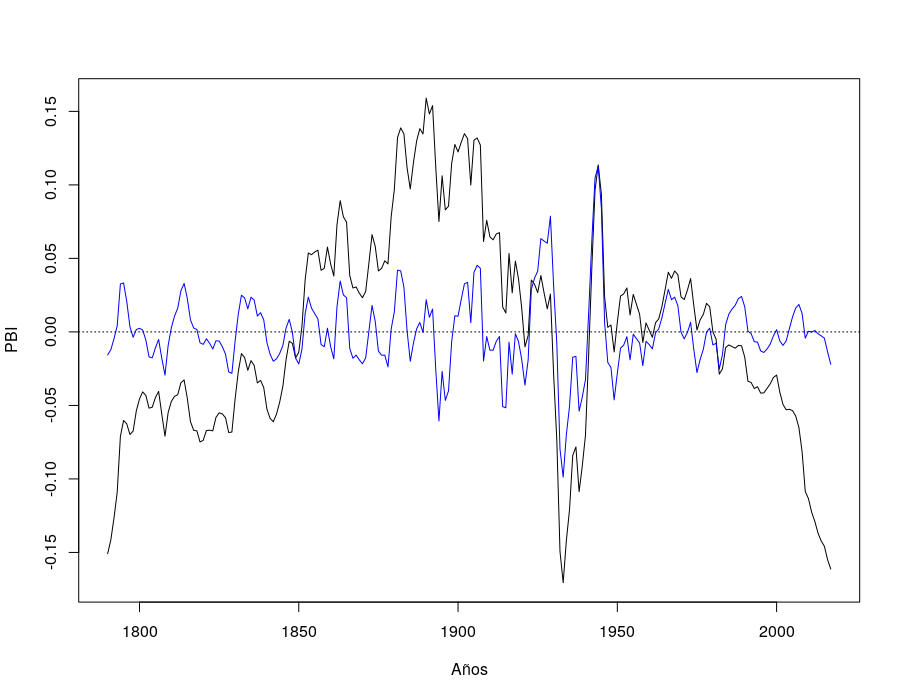
\includegraphics[width=0.49\linewidth]{PBI_fft_resid.png}}
	\subfigure{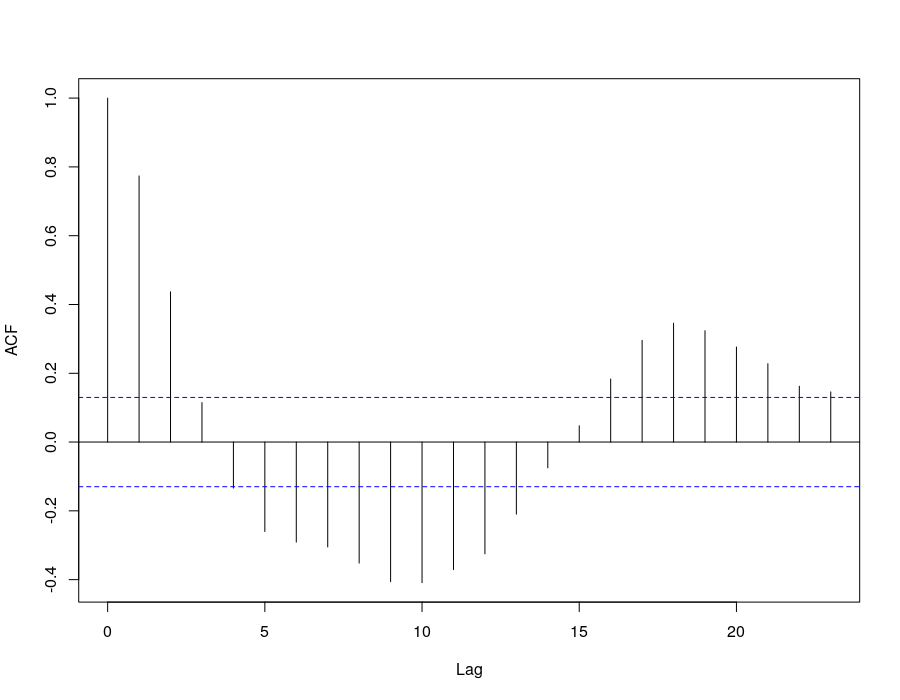
\includegraphics[width=0.49\linewidth]{PBI_resid_acf.png}}
	\caption{PBI centrado con residuos en azul (izquierda) y ACF de los residuos (derecha)}
	\label{fig:PBI_fft_resid}
\end{figure}
%%%%%%%%%%%%%%%%%%%%%%%%%%%%%%%%%%%%%%%%%%%%%%%%%%%%%%%%%%%%%%%%%

\section{Autocorrelación y ARIMA}

En la presente sección se analizará la autocorrelación de las series anteriores, para observar su comportamientos desde un punto de vista sistemático. Para ello también se observará un modelo ARIMA. 

En primer lugar, se calculó la autocorrelación para el total del período en ambas series. Esto se puede observar en la figura \ref{fig:autocorrelacion_tot}. Ambas series tienen un comportamiento similar, con una fuerte correlación con el período anterior, una correlación positiva con respecto a 6 lags, y una relación negativa con 10 lags. 

\begin{figure}[H]
	\centering
	\subfigure[PBI expresado en Oro]{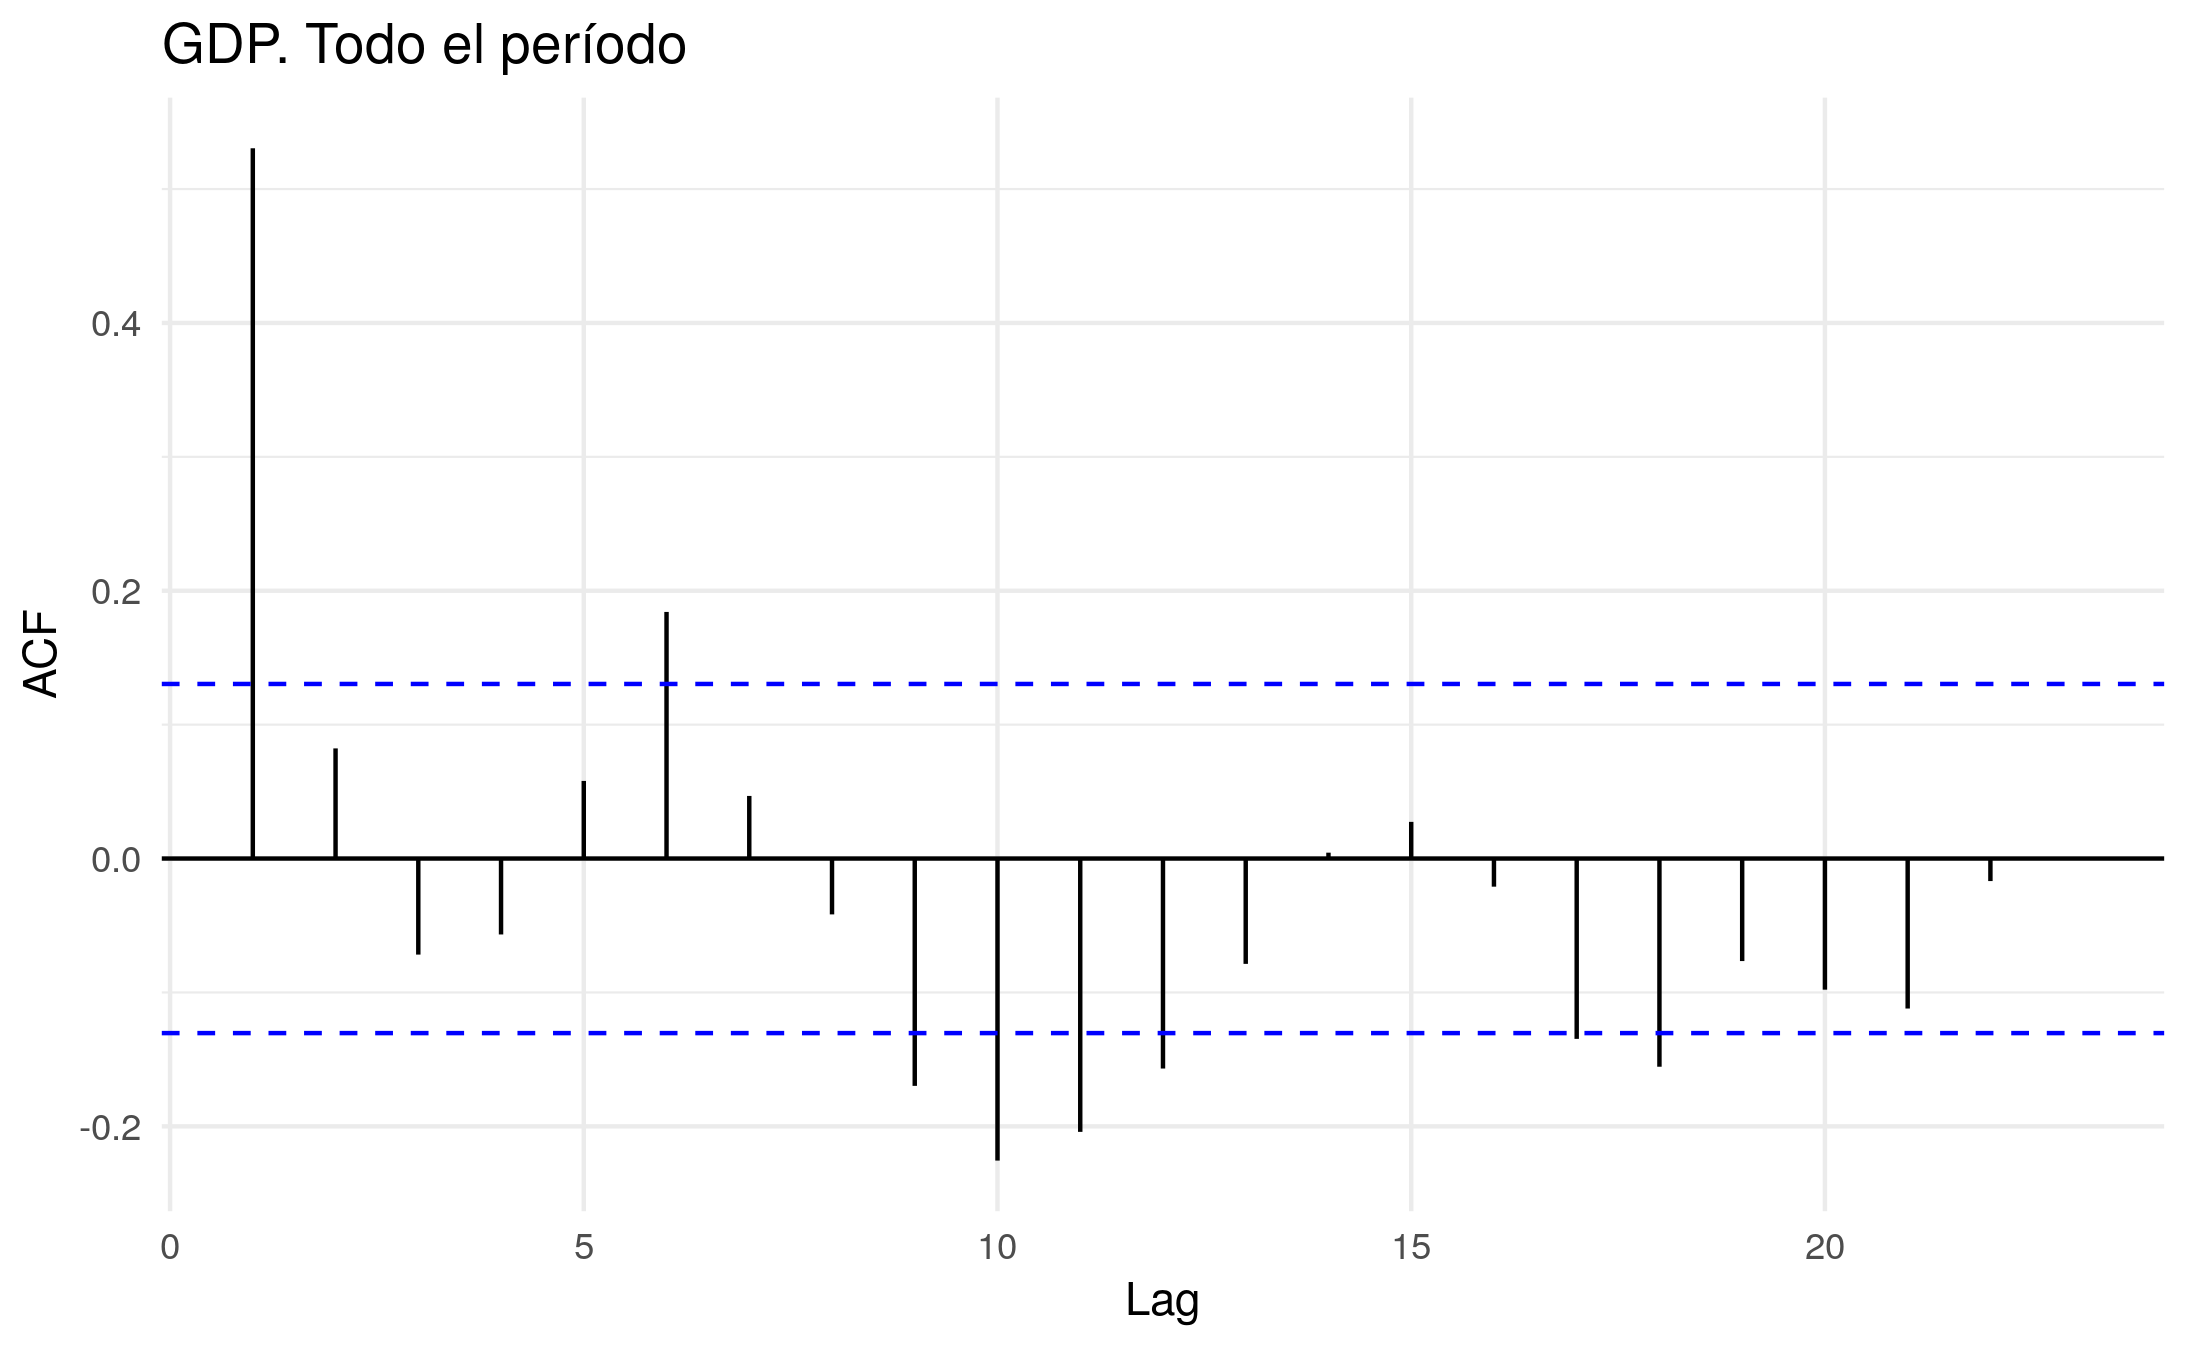
\includegraphics[width=0.75\linewidth]{Autocorrelacion_gdp.png}}
	\subfigure[Salario expresado en Oro]{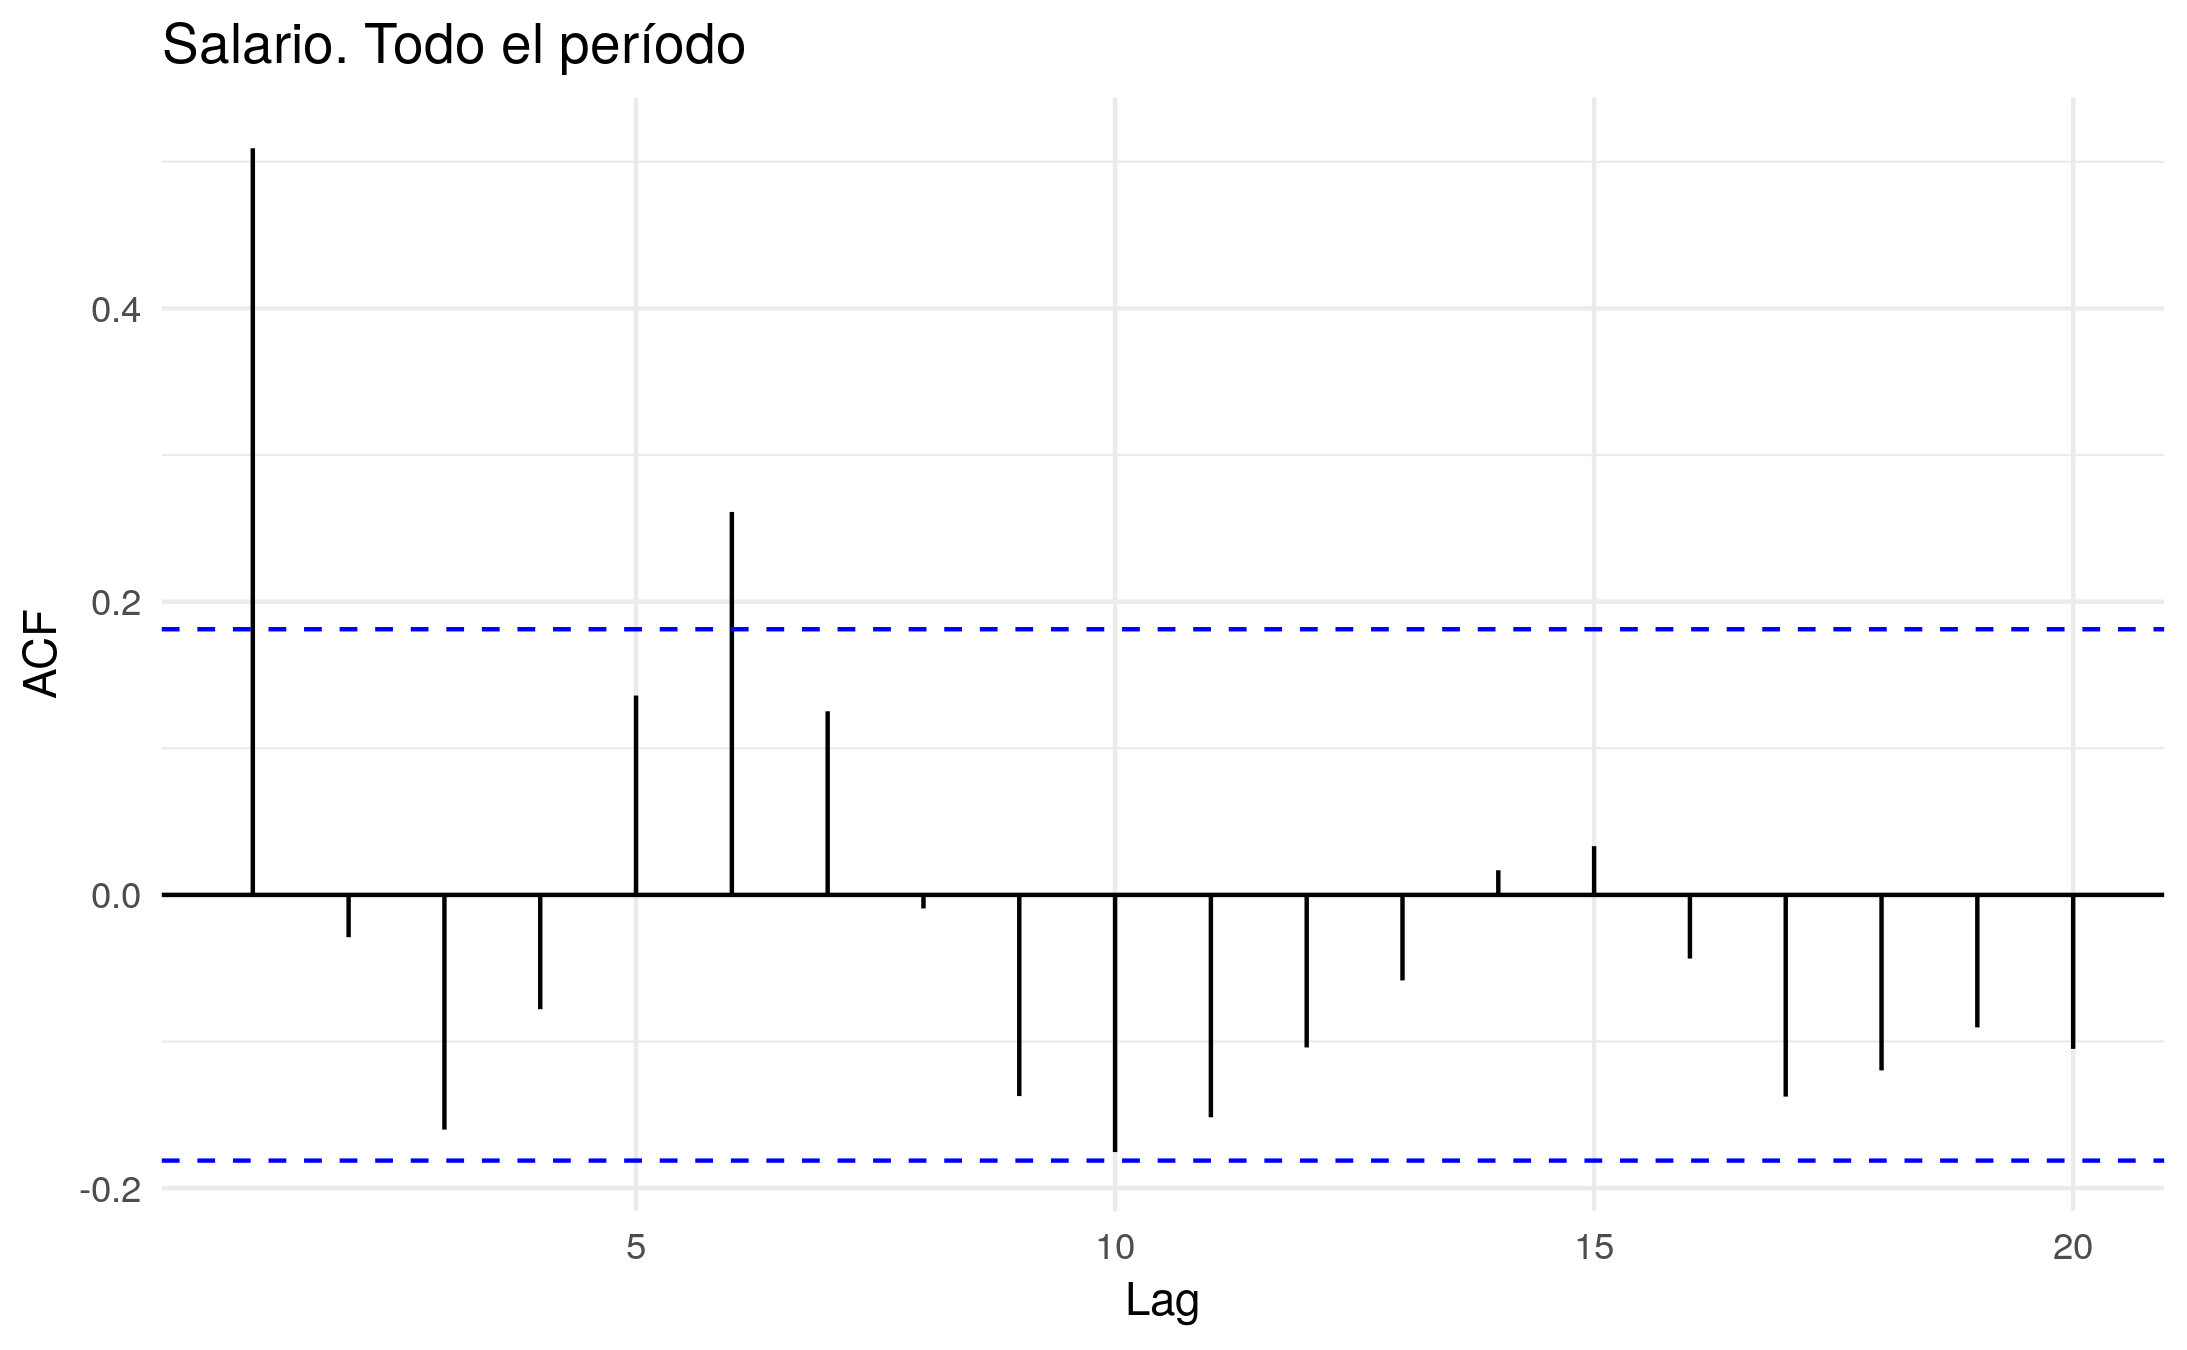
\includegraphics[width=0.75\linewidth]{Autocorrelacion_wg.png}}
	\caption{Autocorrelación de las series} \label{fig:autocorrelacion_tot}
\end{figure}

Sin embargo, dada la importancia de la caída del patrón oro en el 71', se decidió recalcular las autocorrelaciones para antes y después de dicho año. Esto puede observarse en la figura \ref{fig:autocorrelacion_grp}. Aquí nuevamente las series presentan un comportamiento similar entre sí, y sin embargo muy distinto antes y después del período. En particular, antes de 1971 se observa una fuerte correlación positiva con períodos anteriores, en particular para el PBI, que mantiene una relación positiva con hasta los 12 primeros lags. Esto esta reflejando una fuerte tendencia ascendente. Es importante considerar que el quiebre de la serie se realiza en un pico, por lo que antes del 71' queda un fuerte crecimiento observado desde la segunda guerra mundial hasta dicho punto. Lo notable es que ambas series luego de este punto sólo muestran una correlación significativa con el período anterior, es decir parecieran ser un \textit{random walk}.


\begin{figure}[H]
	\centering
	\subfigure[PBI antes 1971]{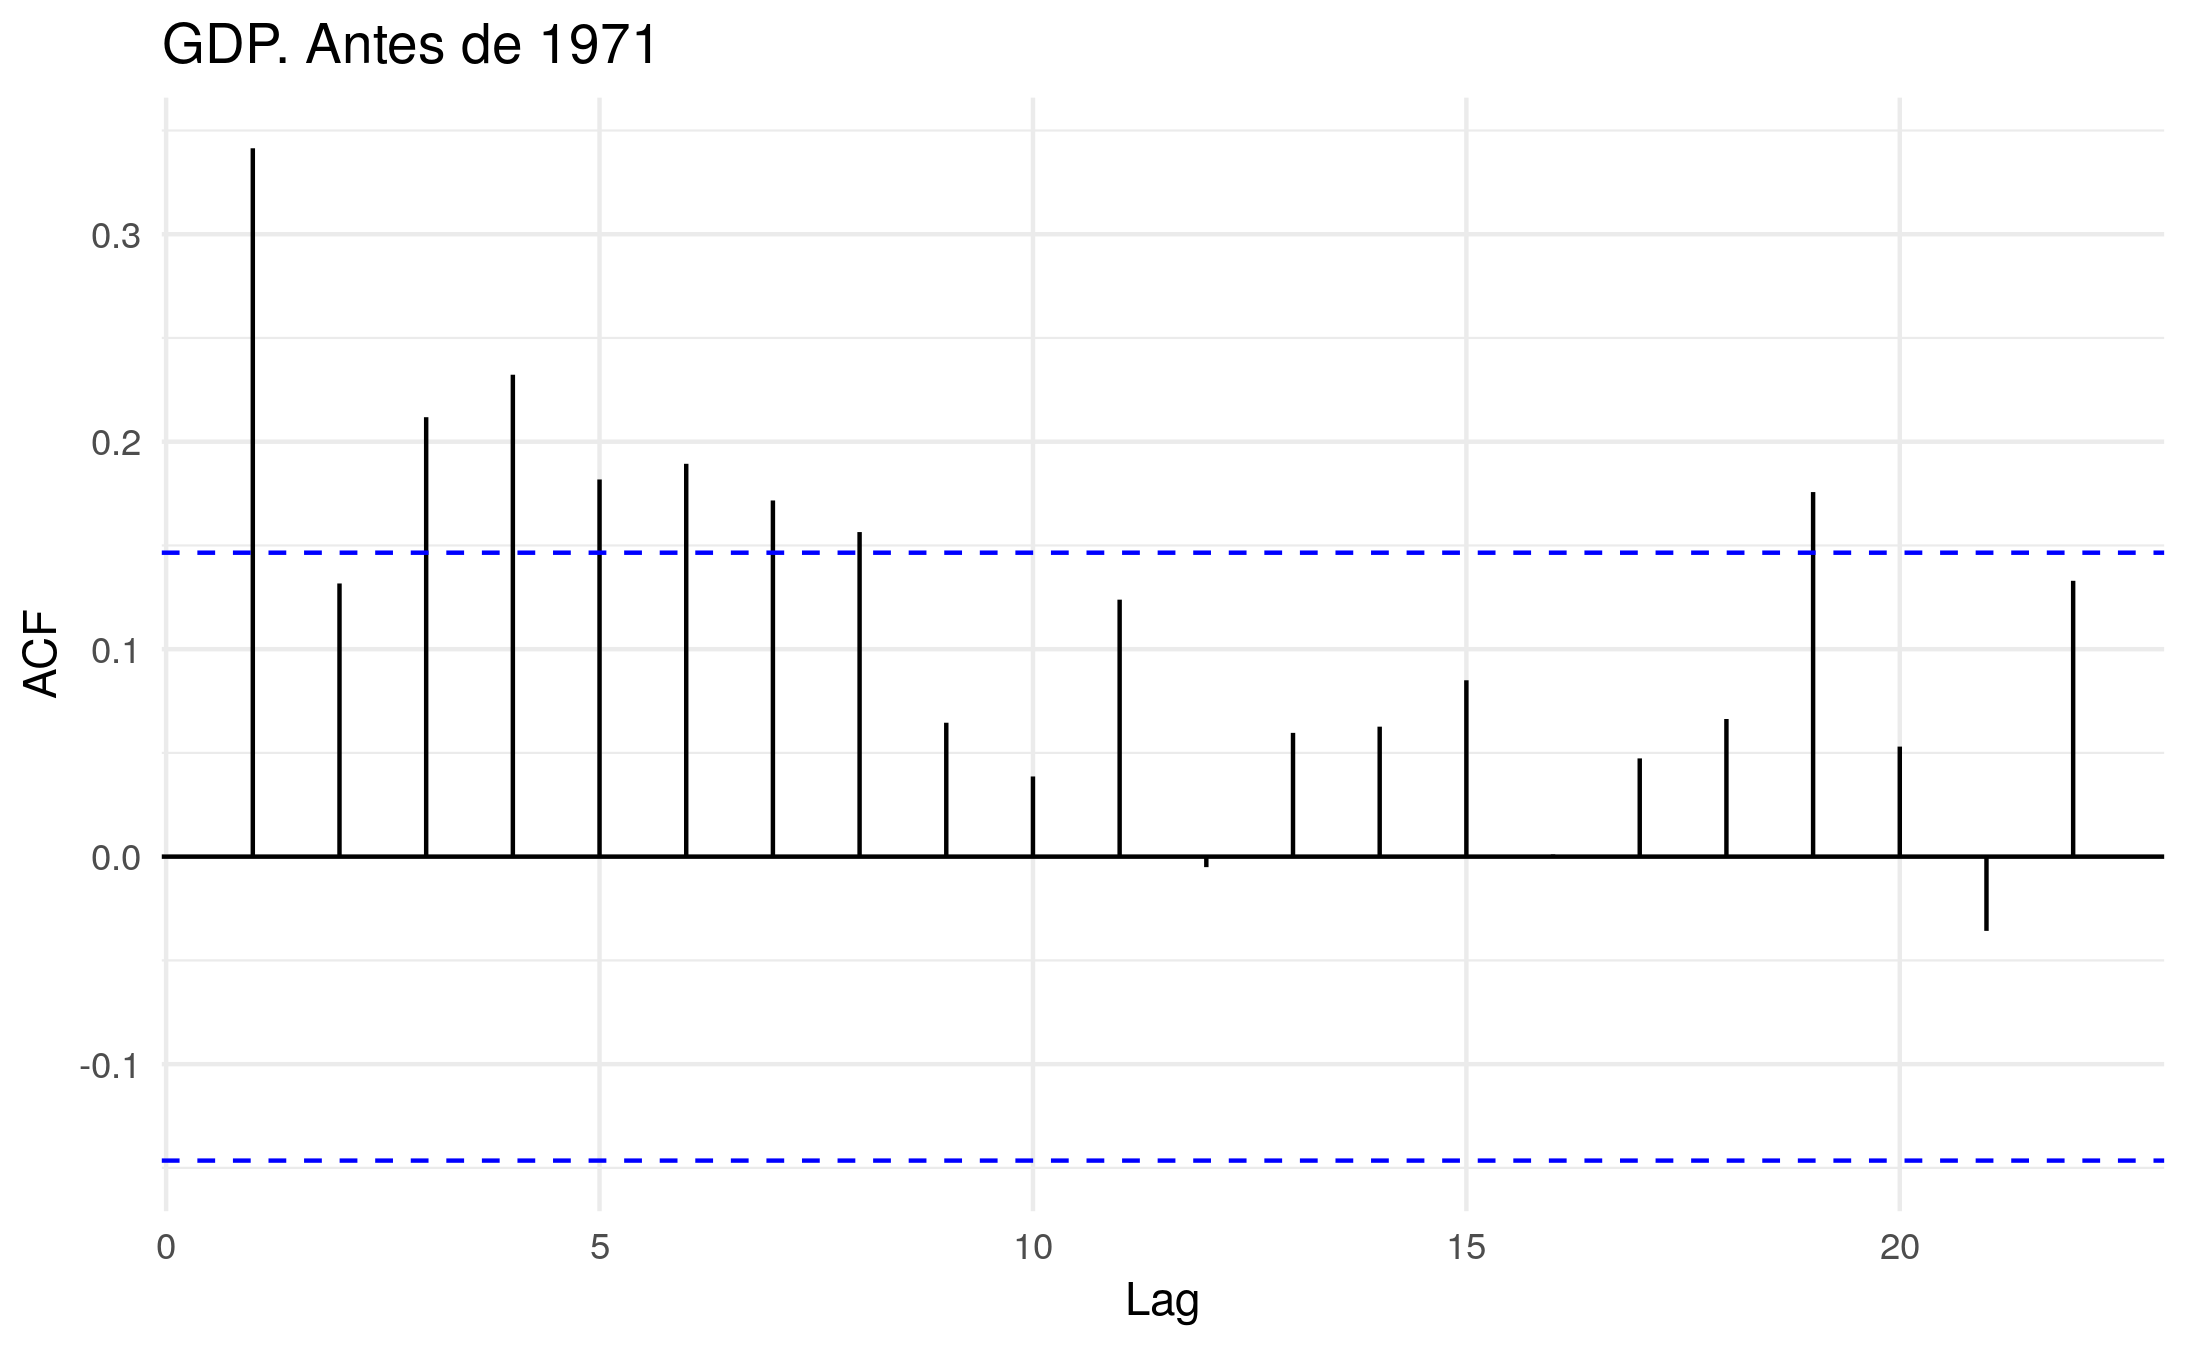
\includegraphics[width=0.49\linewidth]{Autocorrelacion_gdp_pre71.png}}
	\subfigure[PBI después 1971]{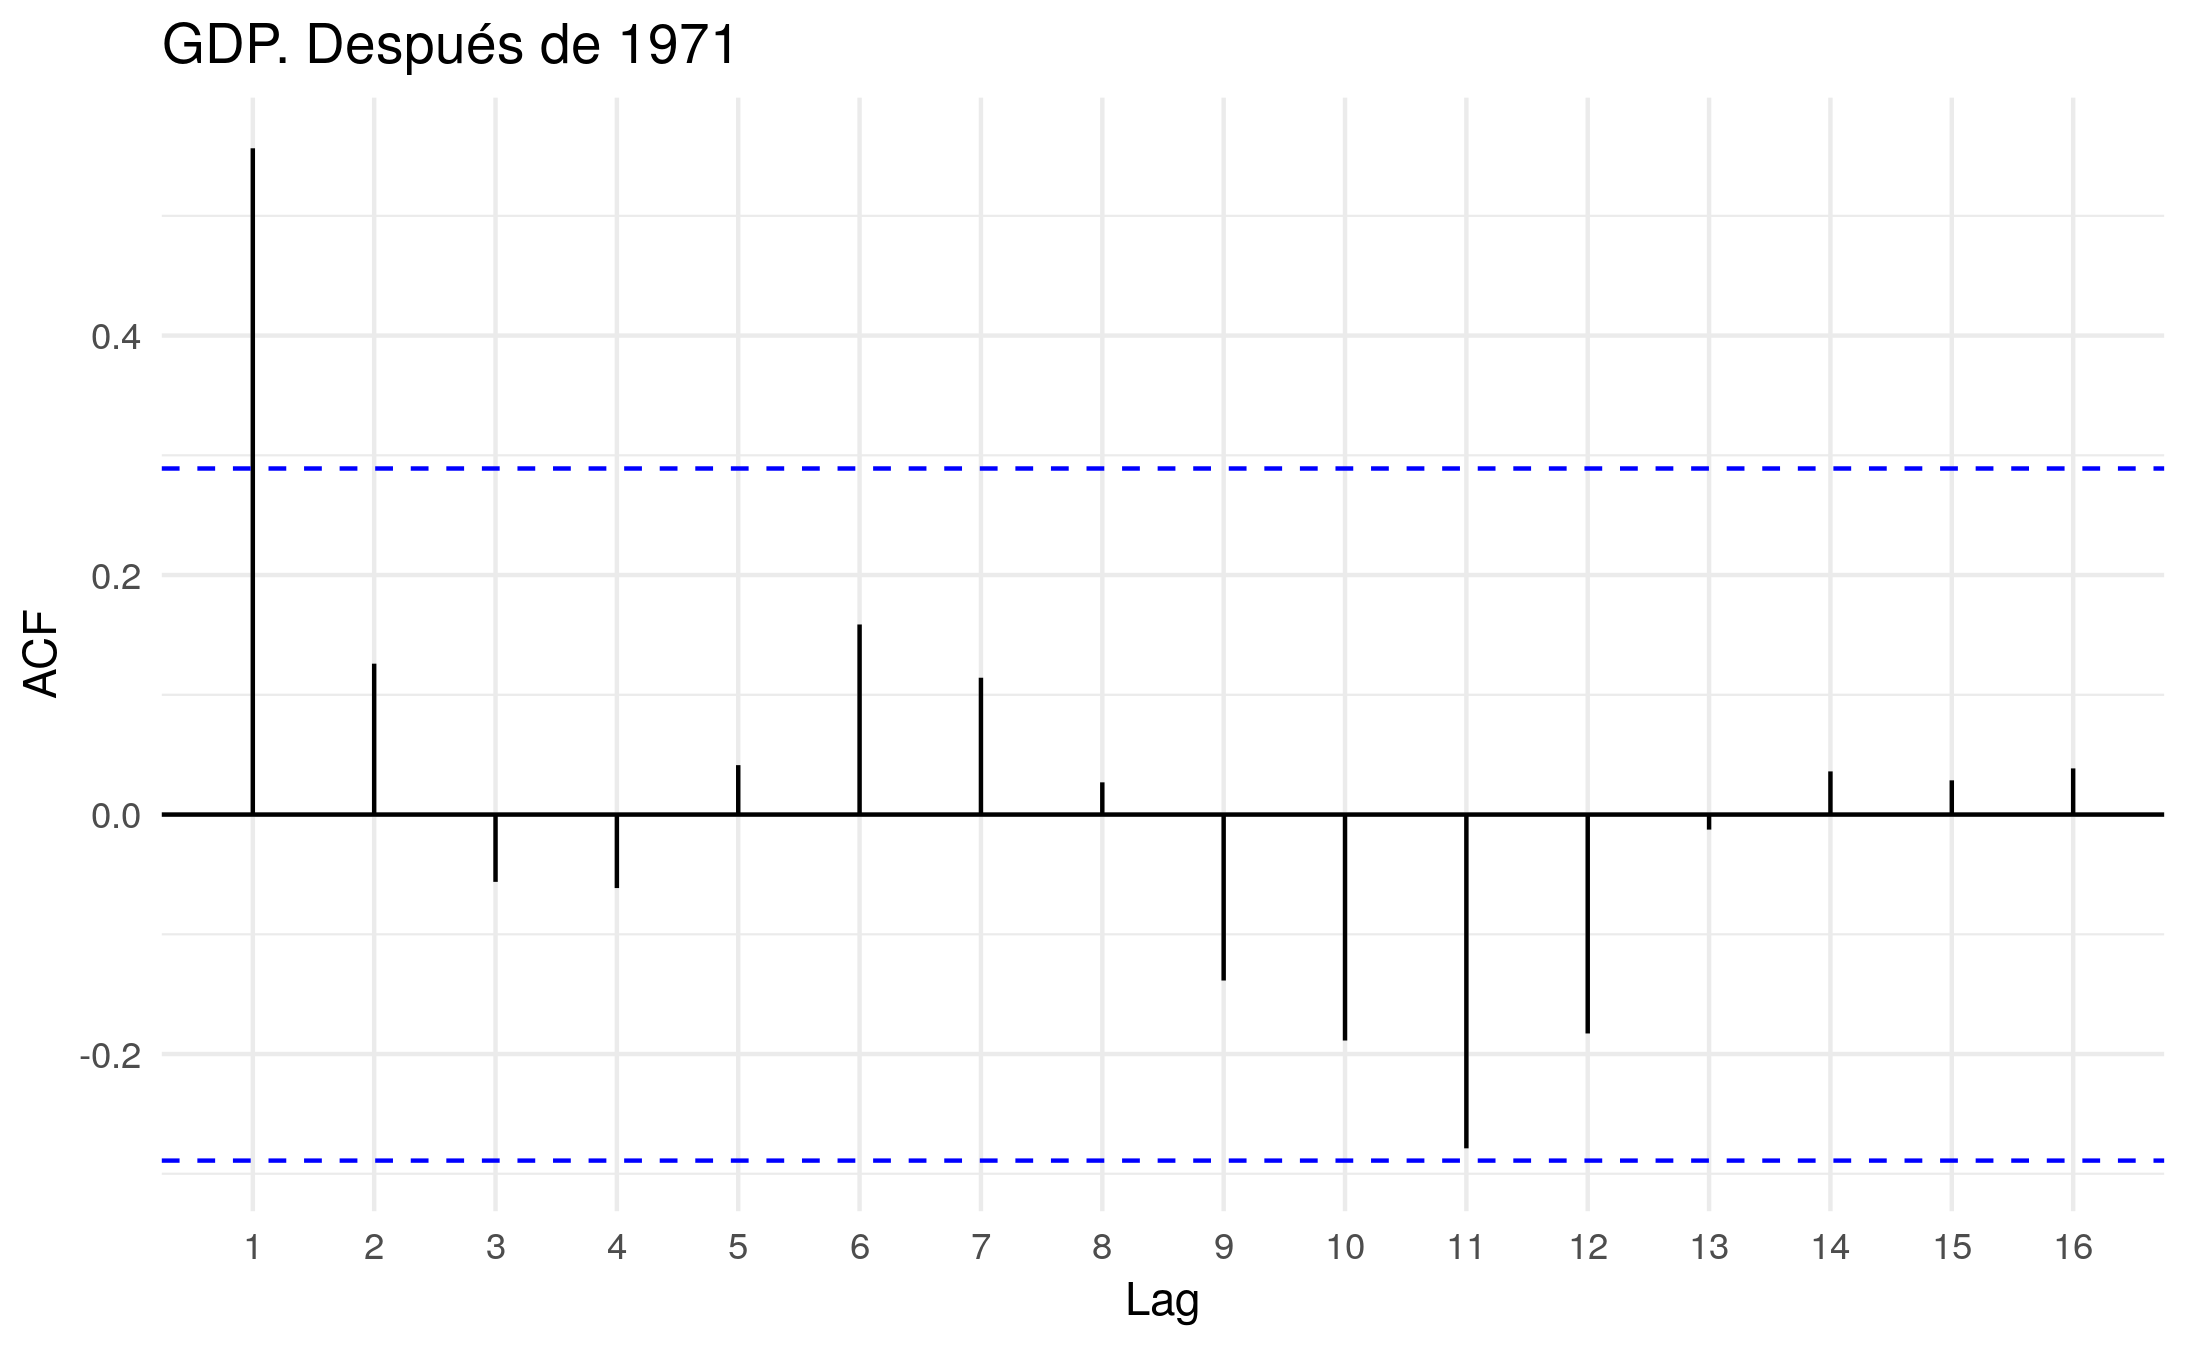
\includegraphics[width=0.49\linewidth]{Autocorrelacion_gdp_post71.png}}
	\subfigure[Salario antes 1971]{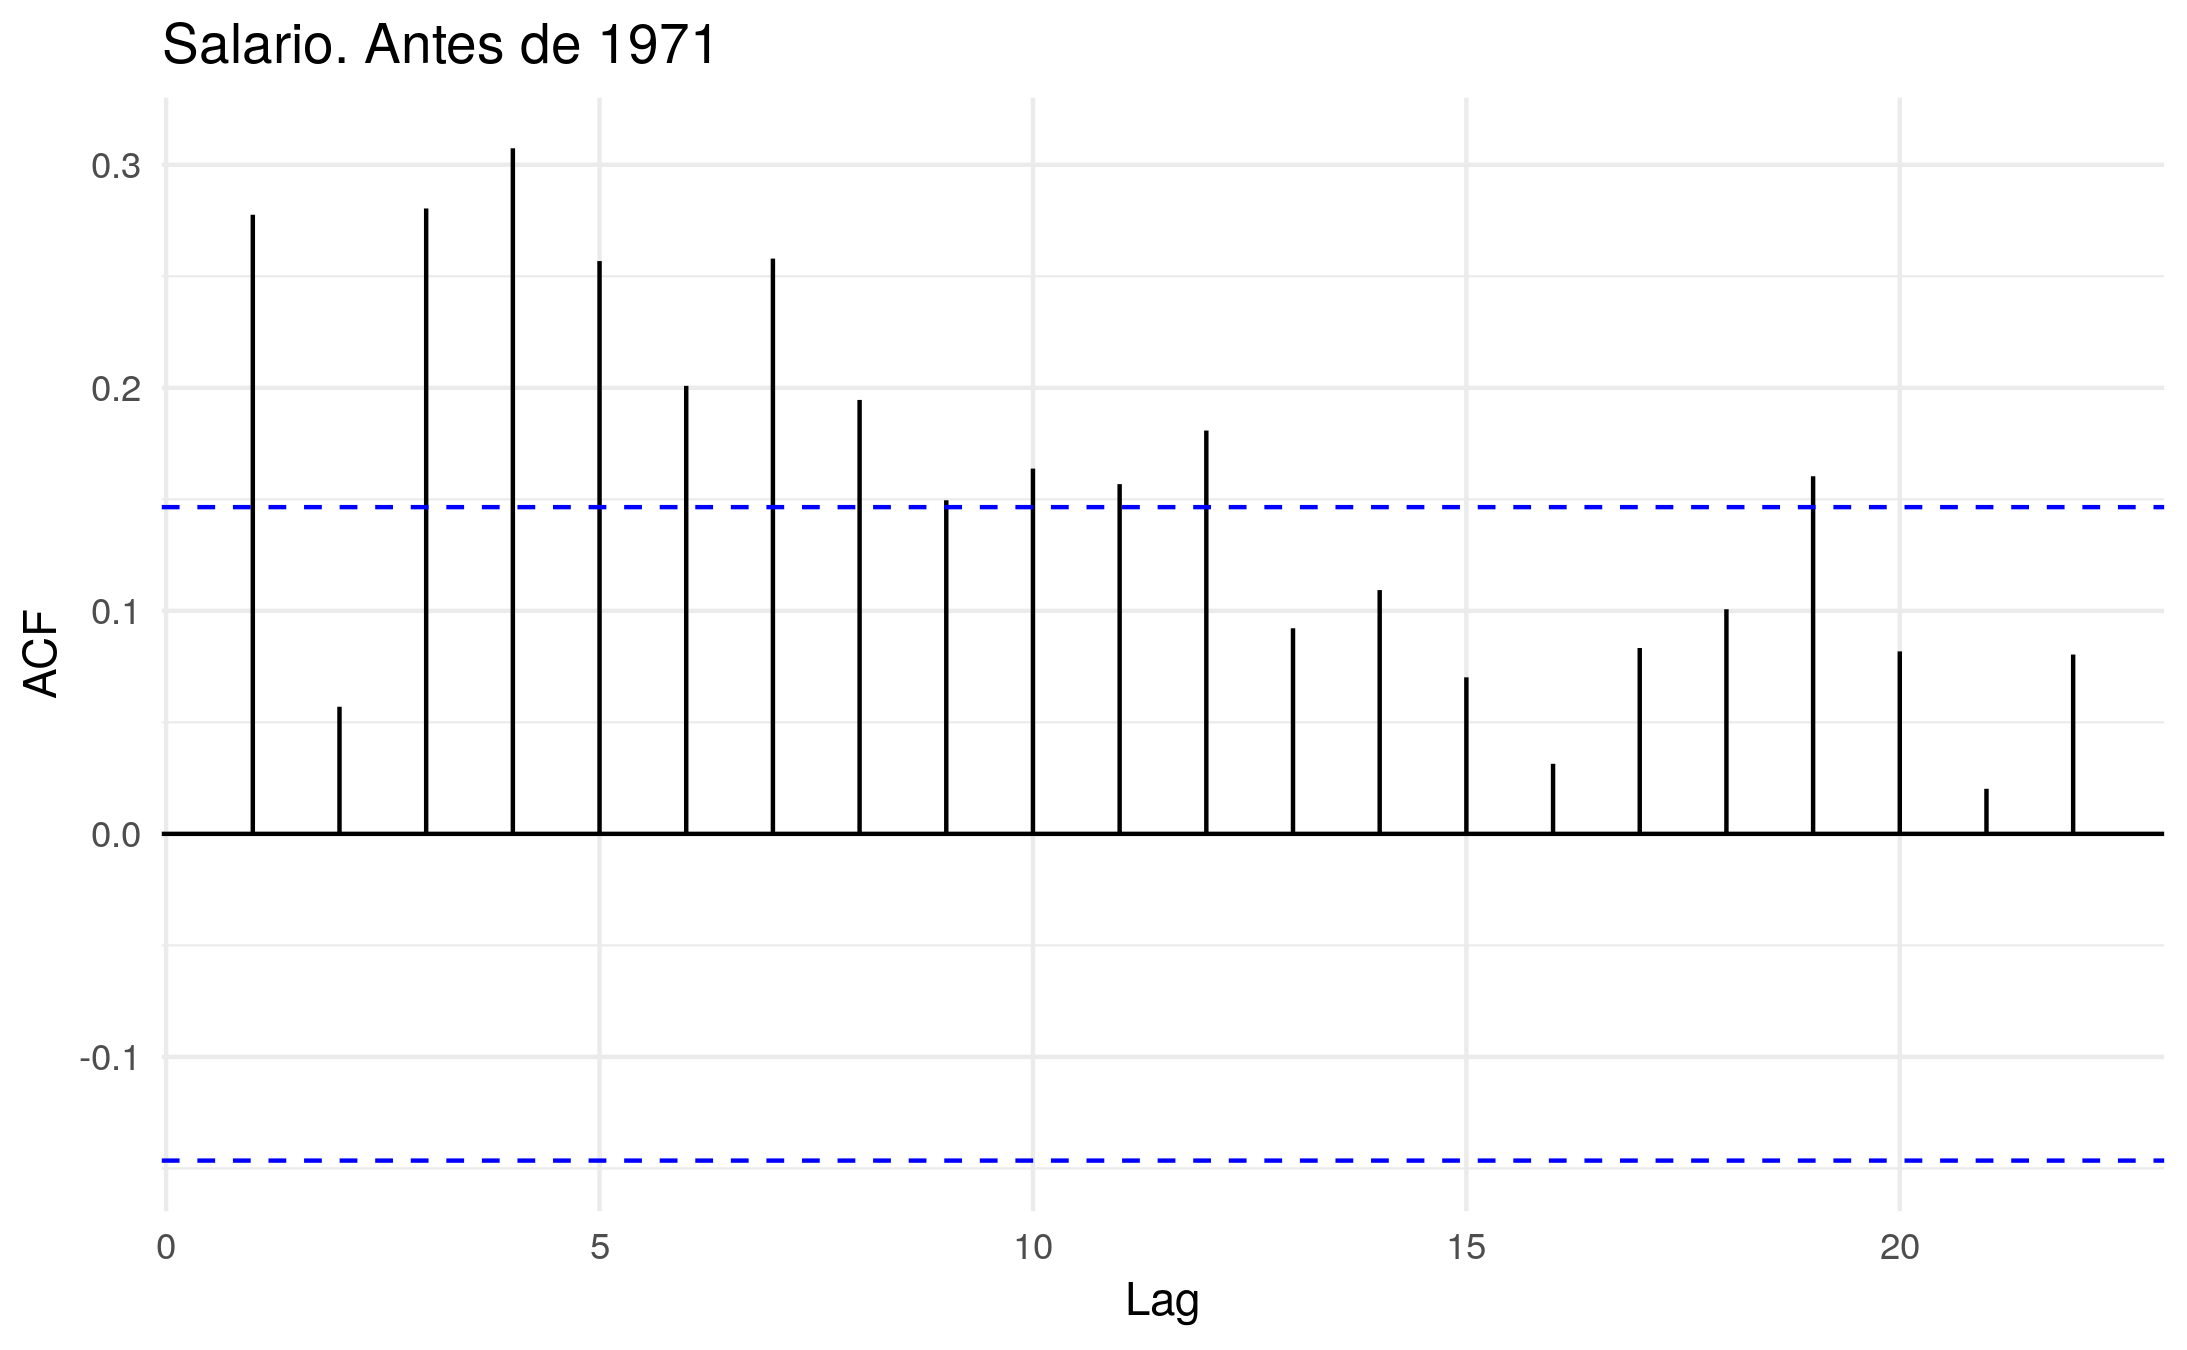
\includegraphics[width=0.49\linewidth]{Autocorrelacion_wg_pre71.png}}
	\subfigure[Salario después 1971]{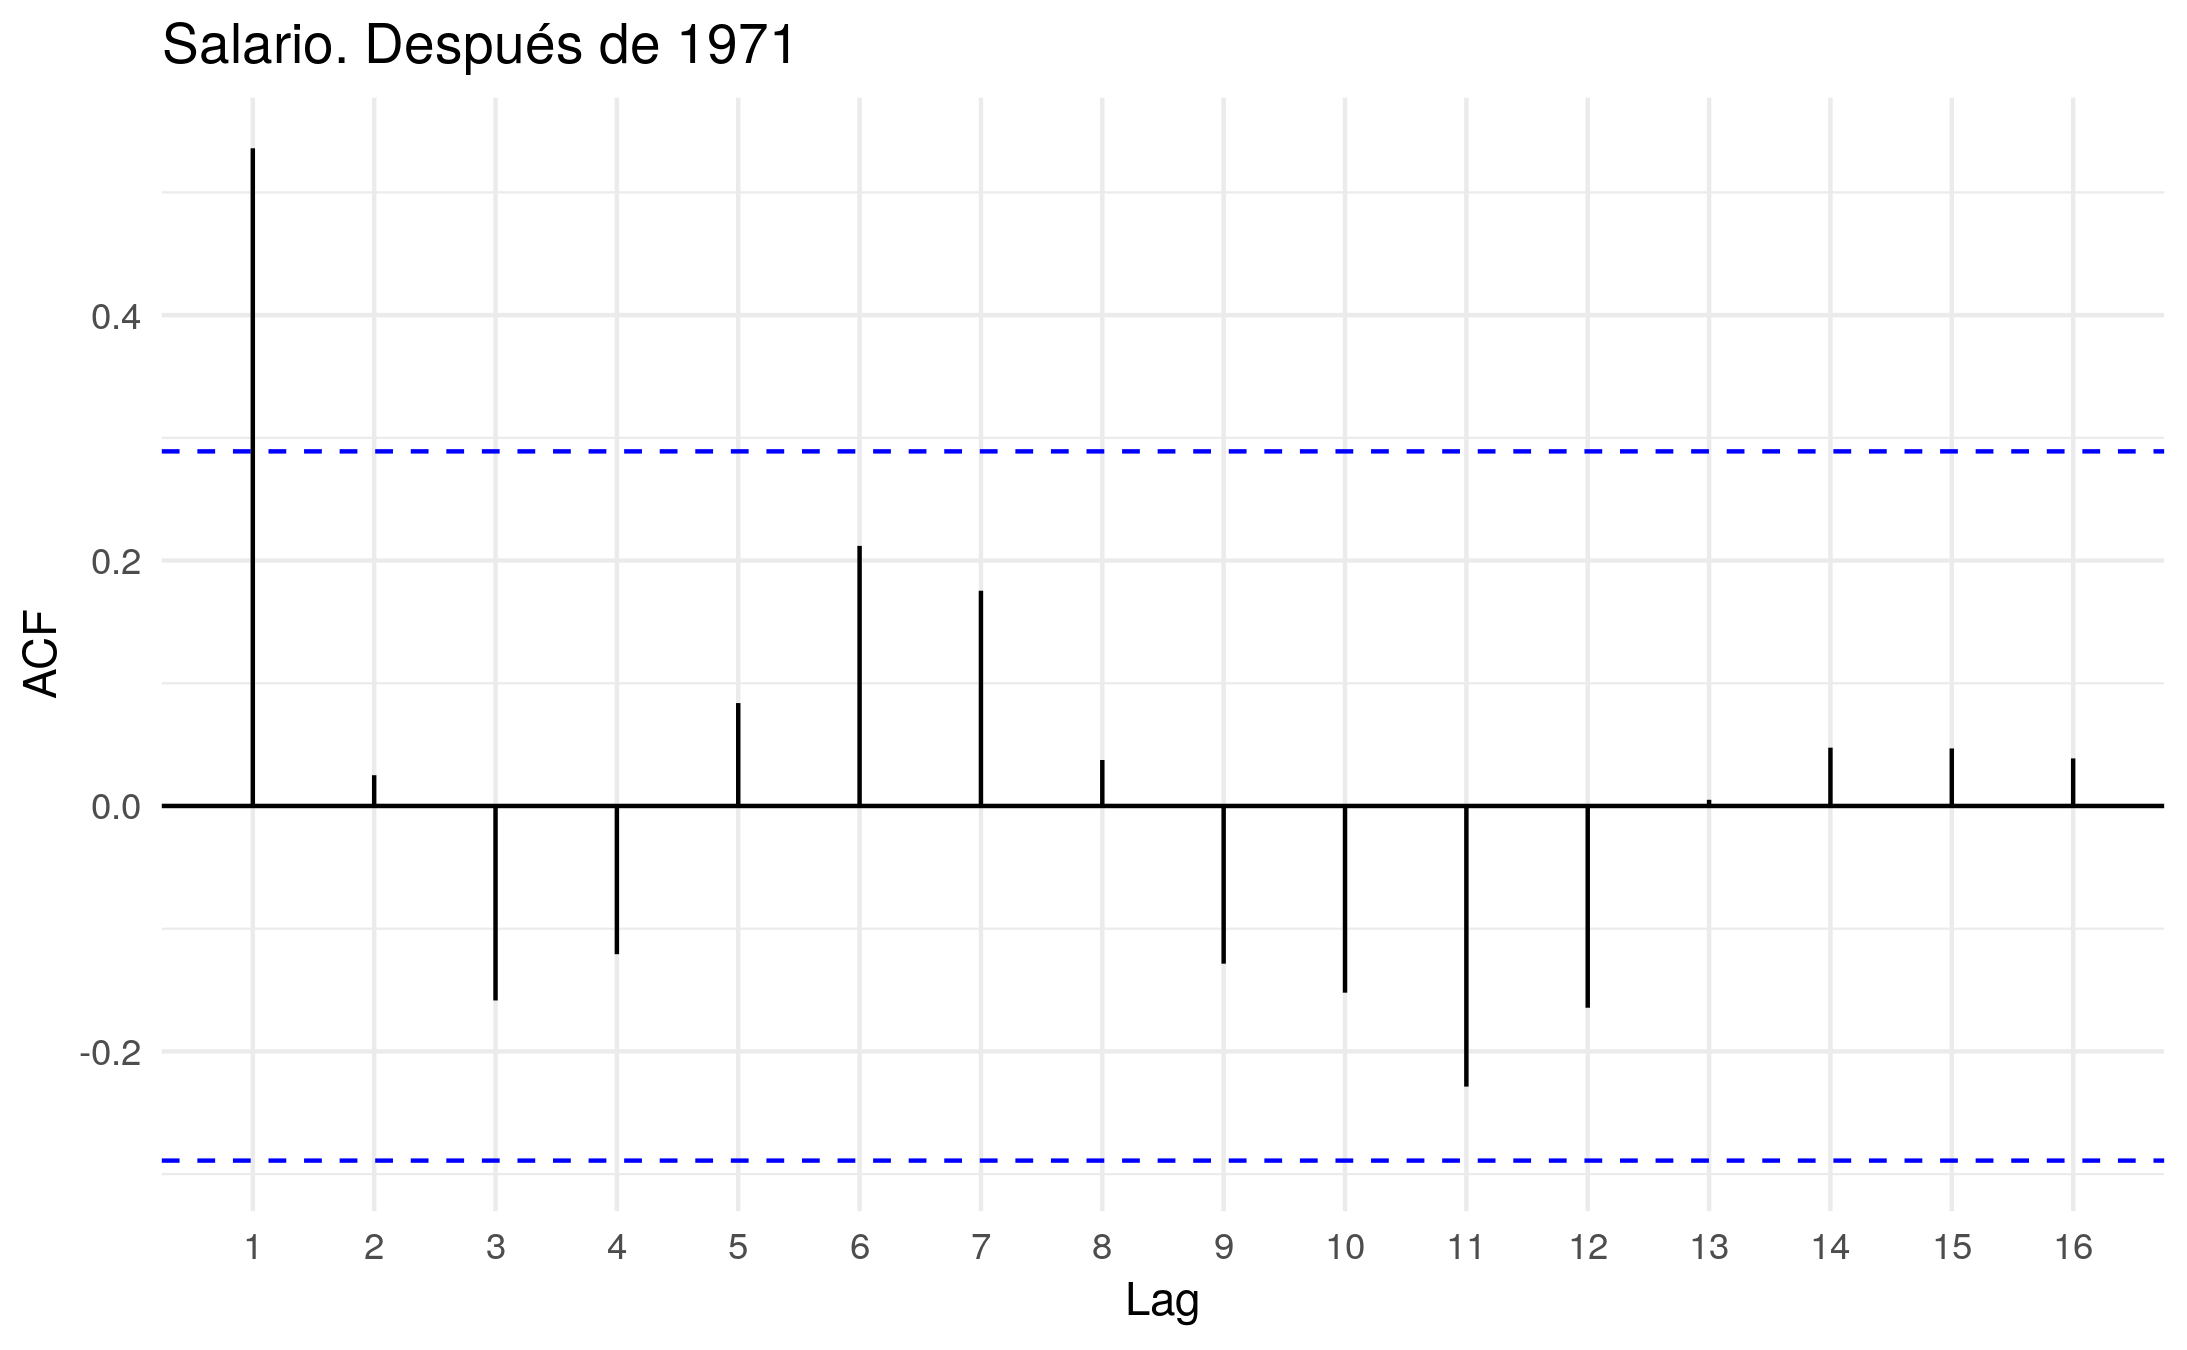
\includegraphics[width=0.49\linewidth]{Autocorrelacion_wg_post71.png}}
	\caption{Autocorrelación de las series} \label{fig:autocorrelacion_grp}
\end{figure}

En la figura \ref{fig:arima} se observa el modelo ajustado por ARIMA para las series en su conjunto y divididas por períodos. 
Los modelos reflejados en \ref{fig:arima_tot} son en ambos casos un modelo ARIMA(1,1,2). Es decir, un modelo autoregresivo de orden 1, integrado de orden uno y Media Móvil de orden 2. Este modelo pareciera ser más volátil que la serie original, en particular para el período posterior a 1971.

\begin{figure}[H]
	\centering
	\subfigure[ARIMA total]{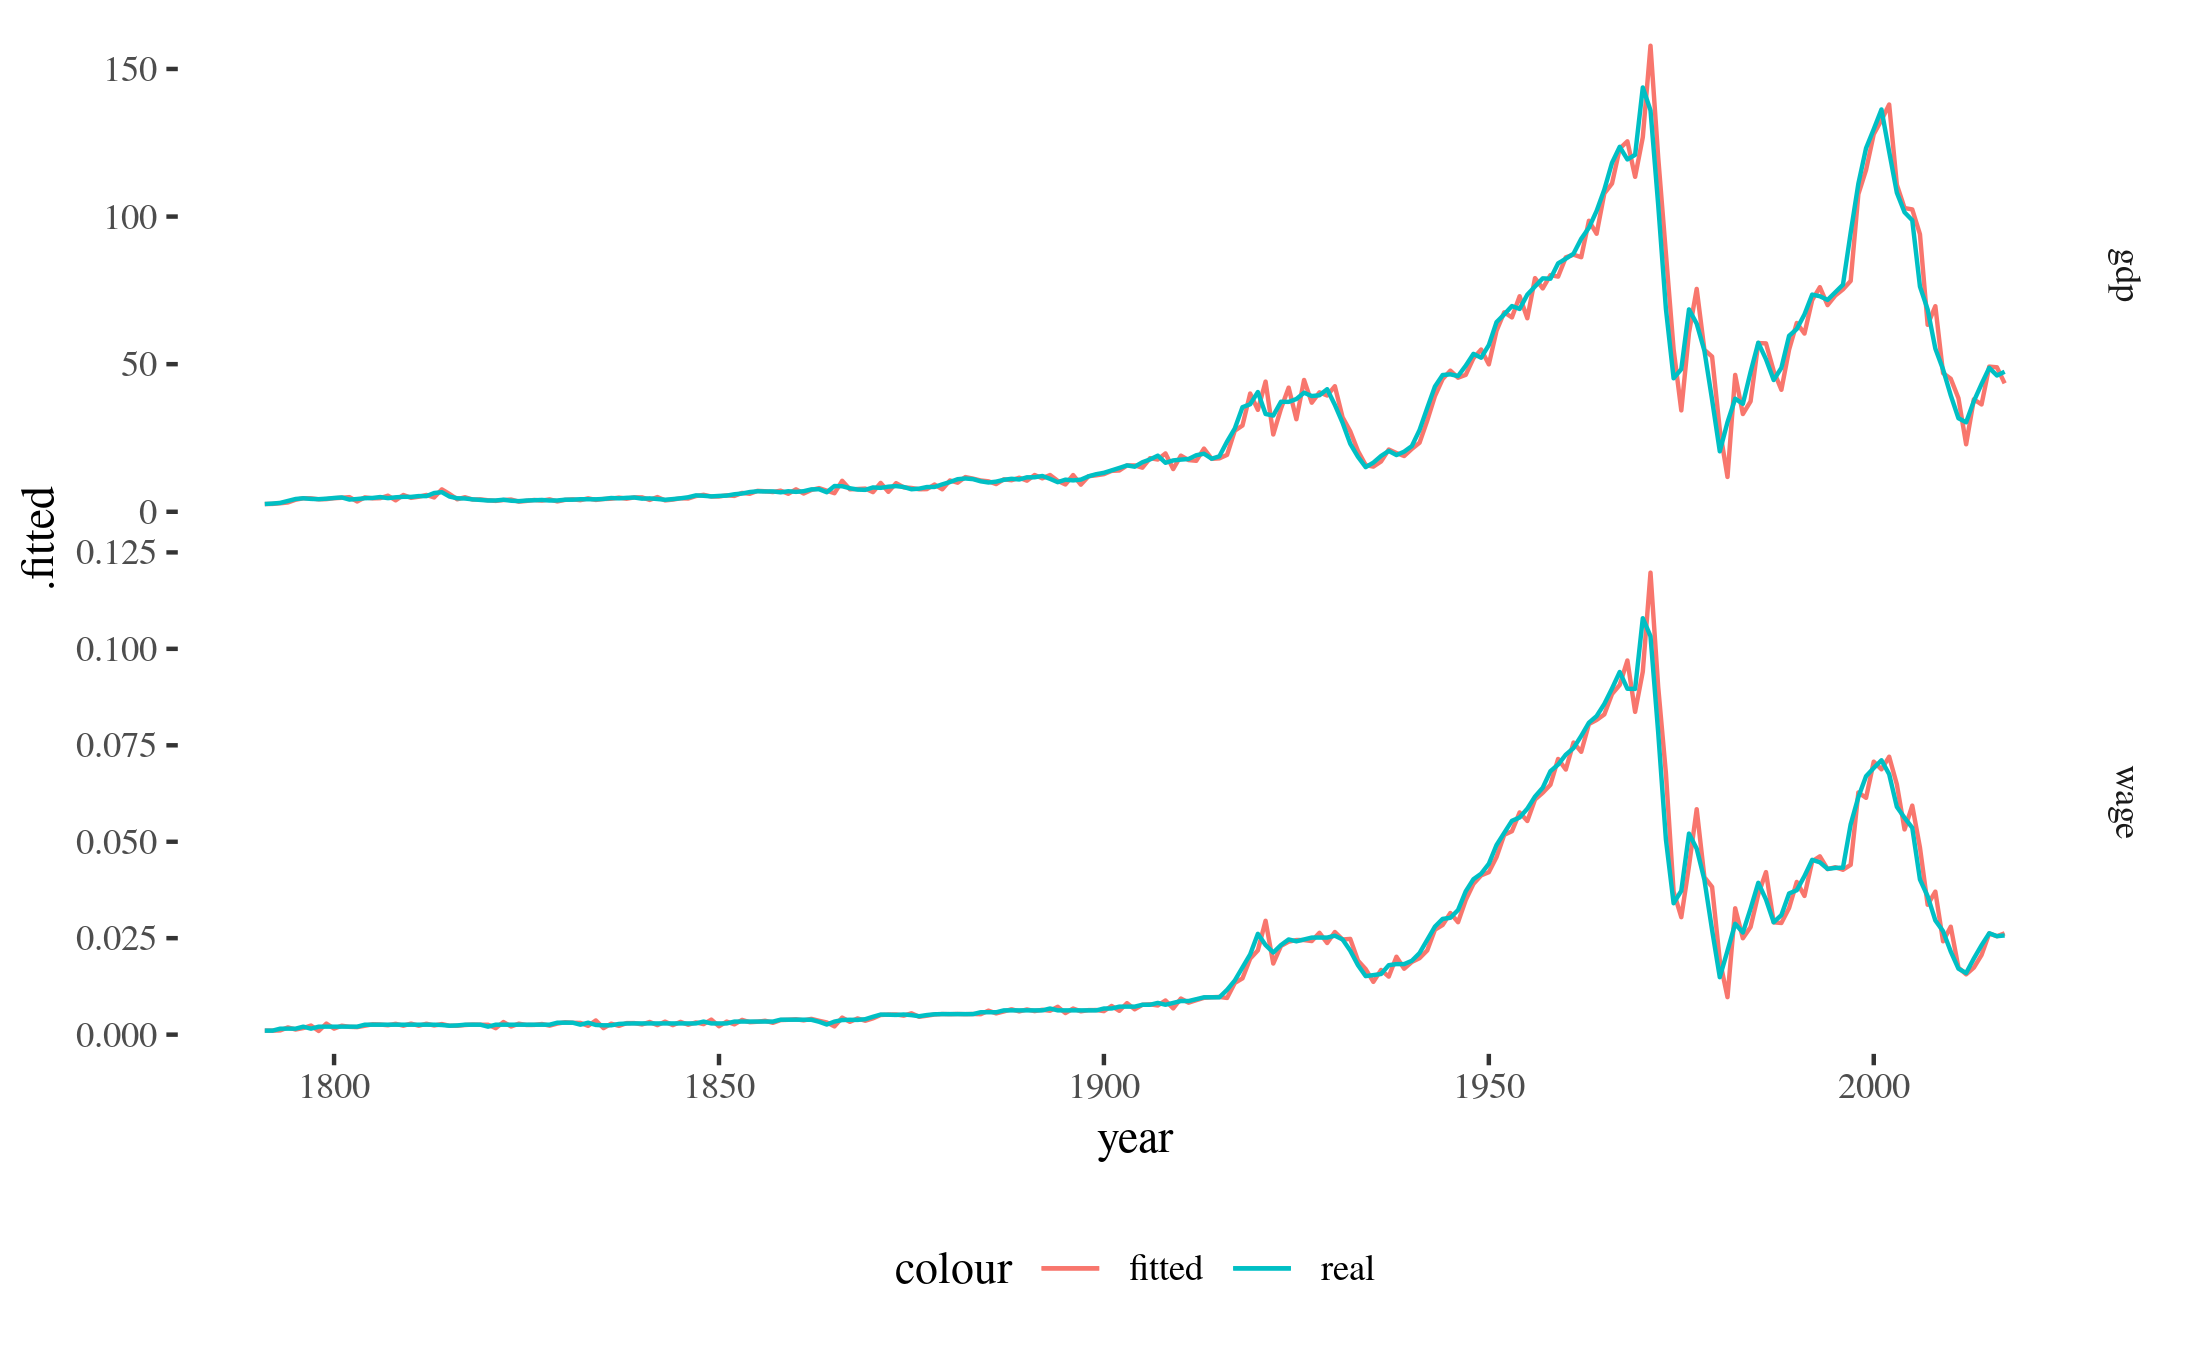
\includegraphics[width=0.8\linewidth]{arima_tot.png}
	\label{fig:arima_tot}}
	\subfigure[ARIMA por grupos]{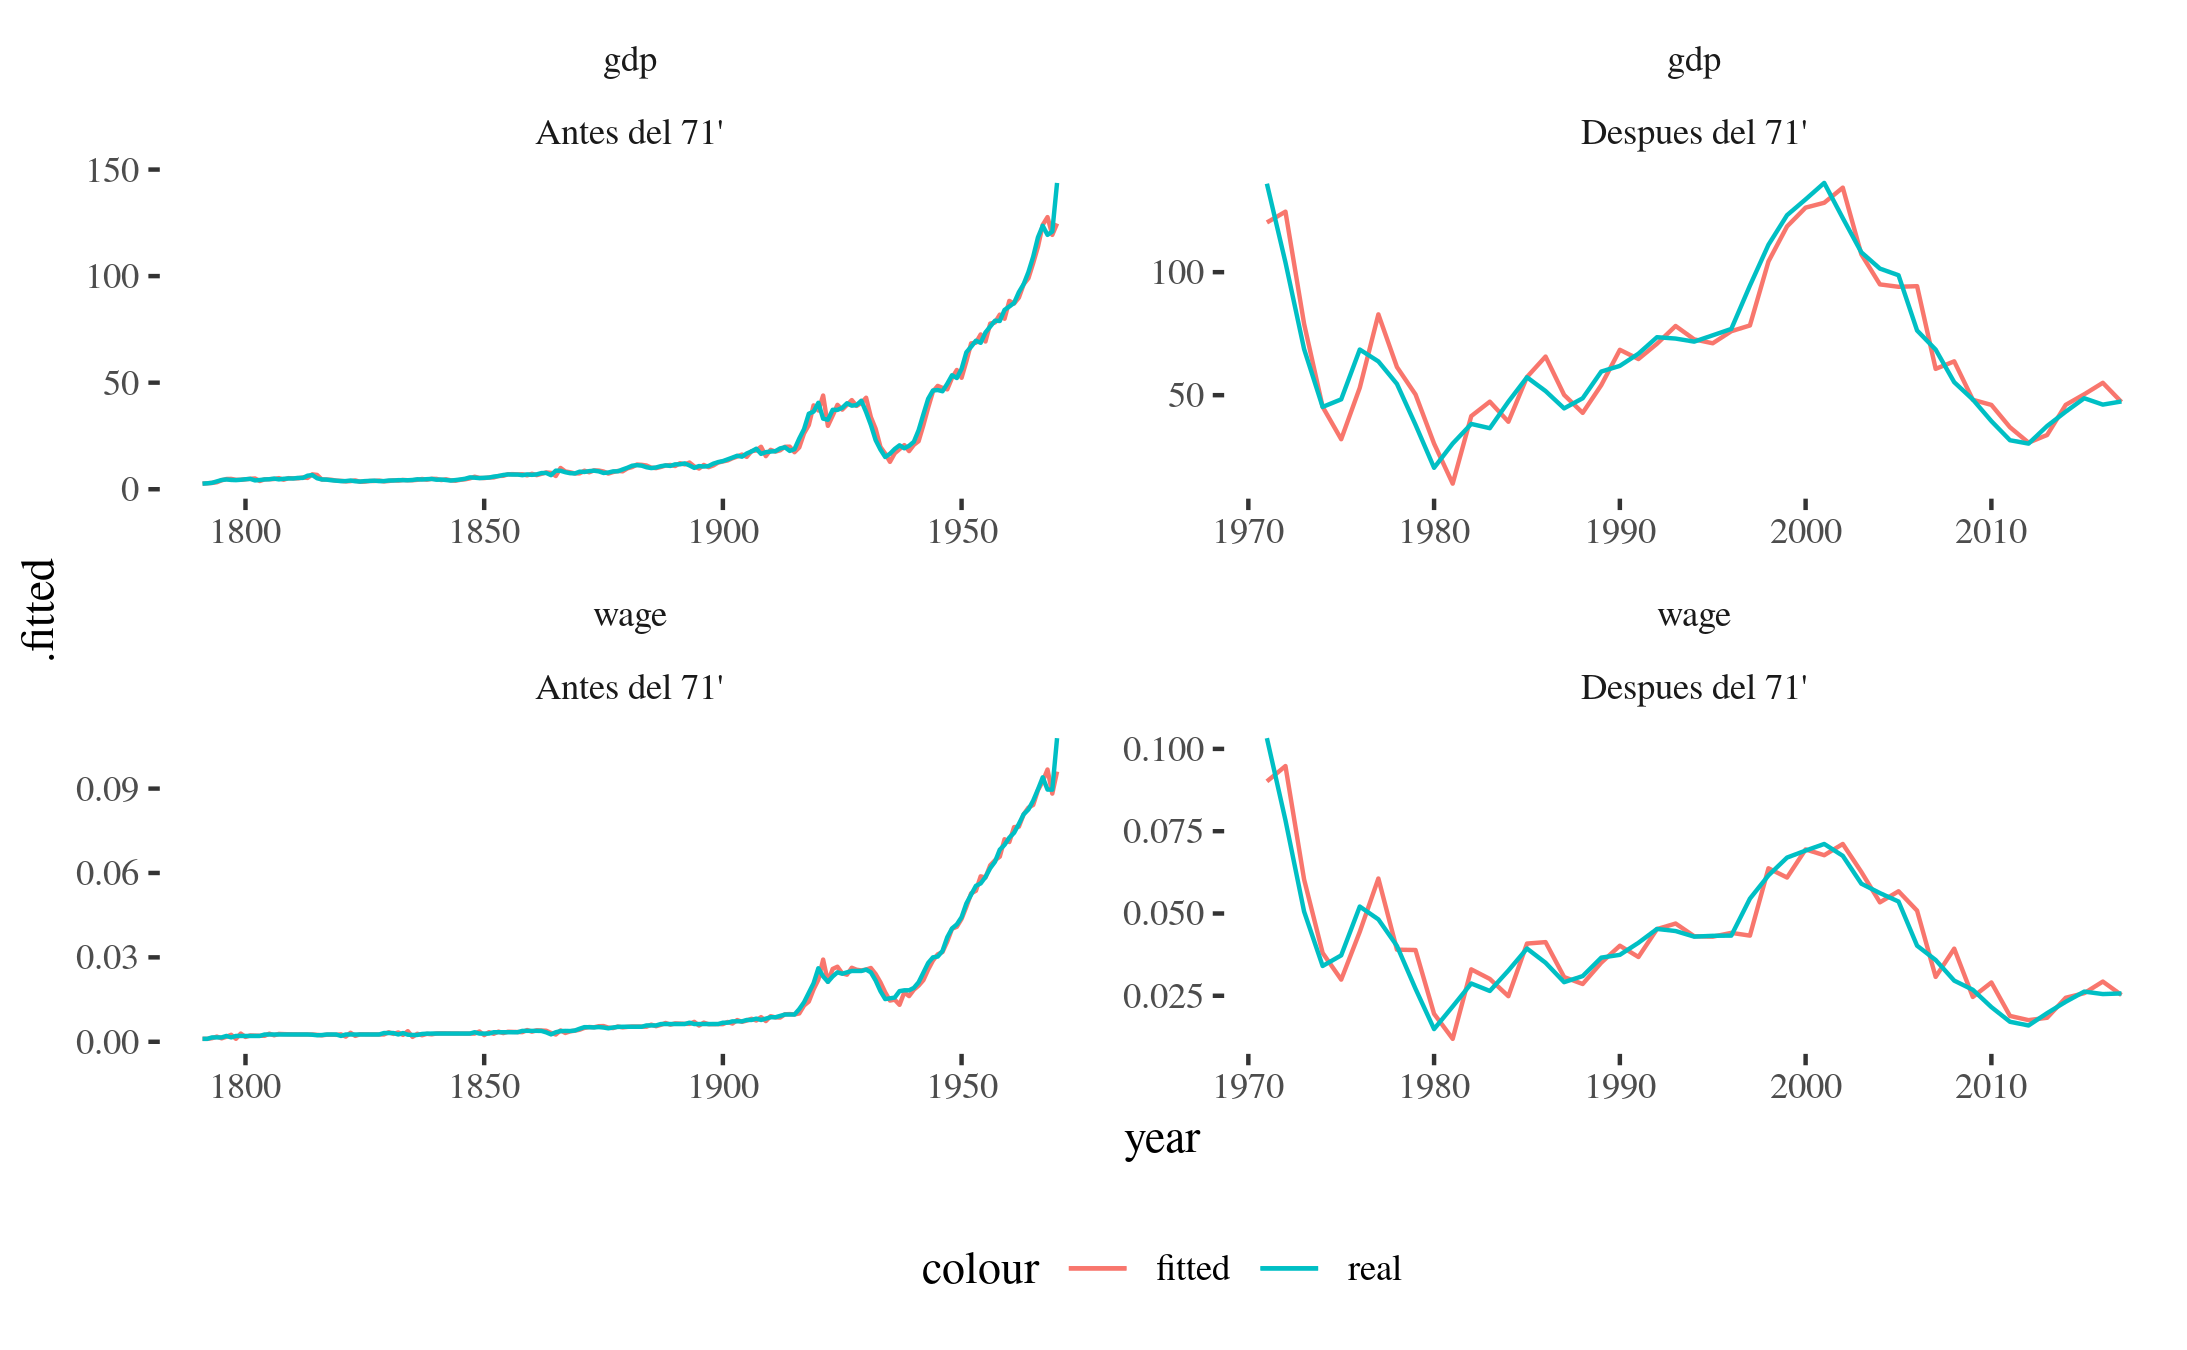
\includegraphics[width=0.8\linewidth]{arima_groups.png}
	\label{fig:arima_grp}}
	\caption{Predicción ARIMA} \label{fig:arima}
\end{figure}

Lo observado en \ref{fig:arima_grp} son los siguientes cuatro modelos: 

\begin{table}[ht]
	\centering
	\begin{tabular}{rlllrr}
		\hline
		& tipo & group & model.desc & sigma & RMSE \\ 
		\hline
		1 & wage & Antes del 71' & ARIMA(2,2,1) & 0.00 & 0.00 \\ 
		2 & wage & Despues del 71' & ARIMA(1,0,2) with non-zero mean & 0.01 & 0.01 \\ 
		3 & gdp & Antes del 71' & ARIMA(0,2,2) & 2.48 & 2.45 \\ 
		4 & gdp & Despues del 71' & ARIMA(2,0,0) with non-zero mean & 9.59 & 9.27 \\ 
		\hline
	\end{tabular}
\end{table}

Se observa tanto un mayor desvío como un mayor error cuadrático medio para ambas series después de 1971. A su vez, las series antes del 71' son integradas de orden dos, producto de lo mencionado arriba de que hasta este punto se toma la fuerte fase ascendente del ciclo en la posguerra, lo que la convierte en una serie divergente. Al contrario, los ARIMA óptimos para las series posteriores a 1971 no requieren ser integrados, sino simplemente tener un término de nivel (\textit{non-zero mean}). A su vez, el modelo también pareciera ser más volátil que las observaciones en este período. Como conclusión, estas herramientas tradicionales de la econometría no bastan para dar cuenta del fenómeno cíclico. 

\section{Wavelets}

Dado que en las secciones previas no se encontró evidencia concluyente en ningún sentido, se decidió explorar nuevas herramientas del análisis de series de tiempo para poder caracterizar el ciclo económico. Los espectogramas producidos mediante \textit{wavelets} parecen ser una herramienta propicia para encontrar ciclos bien definidos a lo largo del período analizado. Las wavelets son un tipo de transformación sobre la serie original que puede pensarse como una rotación de un espacio de funciones a un dominio diferente. A diferencia de la transformada de fourier, que tiene como base de funciones los senos y cosenos, la transformada Wavelet tiene como base de funciones una función particular, con su mismo nombre, Wavelets \cite{castro1995wavelets}. Una base de este tipo se construye a partir de una función madre, que es una onda corta, de duración finita. Es decir, a diferencia de las funciones seno y coseno que se extienden infinitamente,los wavelets tienen \textit{soporte compacto}. Otra característica de las funciones wavelet es que el área debajo de la curva debe ser igual a cero, es decir que esta centrada en cero. Esta función madre se traslada y dilata para construir una base ortonormal. 

Mientras que una transformación de Fourier de una serie desde el dominio del tiempo hacia el dominio de la \textit{frecuencia} toma la forma de:

$$
X(F)=\int_{-\infty}^{\infty} x(t) e^{-j2\pi Ft}dt
$$

La transformada wavelet lleva del dominio del tiempo al dominio de \textit{escala} y \textit{traslación}:

$$
X(a,b)=\int_{-\infty}^{\infty} x(t) \psi^*_{a,b}(t)dt
$$

La escala describe la frecuencia (inversa de la extensión o período) del ciclo, mientras que la traslación describe el movimiento a lo largo de la serie. Dado que las series de baja frecuencia (ciclos más largos) ocupan una porción mayor de la serie, son más difíciles de ubicar en un momento particular del tiempo. El wavelet logra definir la presencia de una determinada frecuencia en un determinado momento del tiempo. Por lo mencionado, la resolución en bajas frecuencias es mala en el dominio del tiempo, pero buena en el dominio de la frecuencia, mientras que los ciclos de alta frecuencia tienen alta resolución en el dominio del tiempo, pero menos resolución en el dominio de la frecuencia. Si lo comparamos con las transformadas de fourier, podríamos pensar que ésta tiene muy alta resolución en el dominio de la frecuencia, pero ninguna resolución en el dominio del tiempo. 

También es posible entender a los Wavelets como un análisis de la correlación entre una serie de tiempo, y una cierta función ondulatoria compacta, en un momento del tiempo y una frecuencia determinada. Las traslaciones lo generan es un corrimiento de la función ondulatoria, y por lo tanto podemos calcular la correlación para todo el rango temporal. El reescalado modifica la frecuencia de la función ondulatoria, lo que permite calcular la correlación para varias frecuencias de onda diferentes. La cantidad de datos disponibles es la que define la capacidad de reescalar la función base, es decir, cuan bajas son las frecuencias mínimas que se puede analizar. Finalmente lo que obtenemos es un valor de la asociación lineal entre la serie original y la función base, para cada valor del tiempo y la frecuencia.  

La función base que utilizamos para el presente trabajo es la denominada \textit{Morlet Wavelet}, que tal como se implementa en la librería WaveletComp \citep{Roesch2018} tiene la siguiente forma funcional:
$$
\psi(t)=\pi^{-\frac{1}{4}}e^{i\omega t}e^{\frac{-t^2}{2}}
$$

Donde $\omega$ es la frecuencia angular (tasa de rotación en radianes por unidad de tiempo). Esta es una función continua, compleja, frecuentemente utilizada en la literatura \citep{conraria2011continuous}. Por su parte, las base a partir de la traslación, $a$, y el escalado, $b$, implementada es:

$$
X(a,b)=\sum_{t} x(t)   \frac{1}{b} \psi^*\left(\frac{t-a}{b}\right)dt
$$

Visualmente, las traslaciones y reescalados de la función base se pueden observar en la figura \ref{fig:morlet}. Allí se aprecia que las traslaciones se definen en el dominio del tiempo, mientras que los reescalados lo hacen en el dominio de la frecuencia. Luego, si se reconstruye el plano tiempo-frecuencia y se calcula la correlación de cada punto del dicho plano con la serie original, se obtiene una nueva dimensión que representa el grado de ajuste de nuestra serie a cada frecuencia, para los distintos momentos del tiempo. 

\begin{figure}[H]
	\centering
	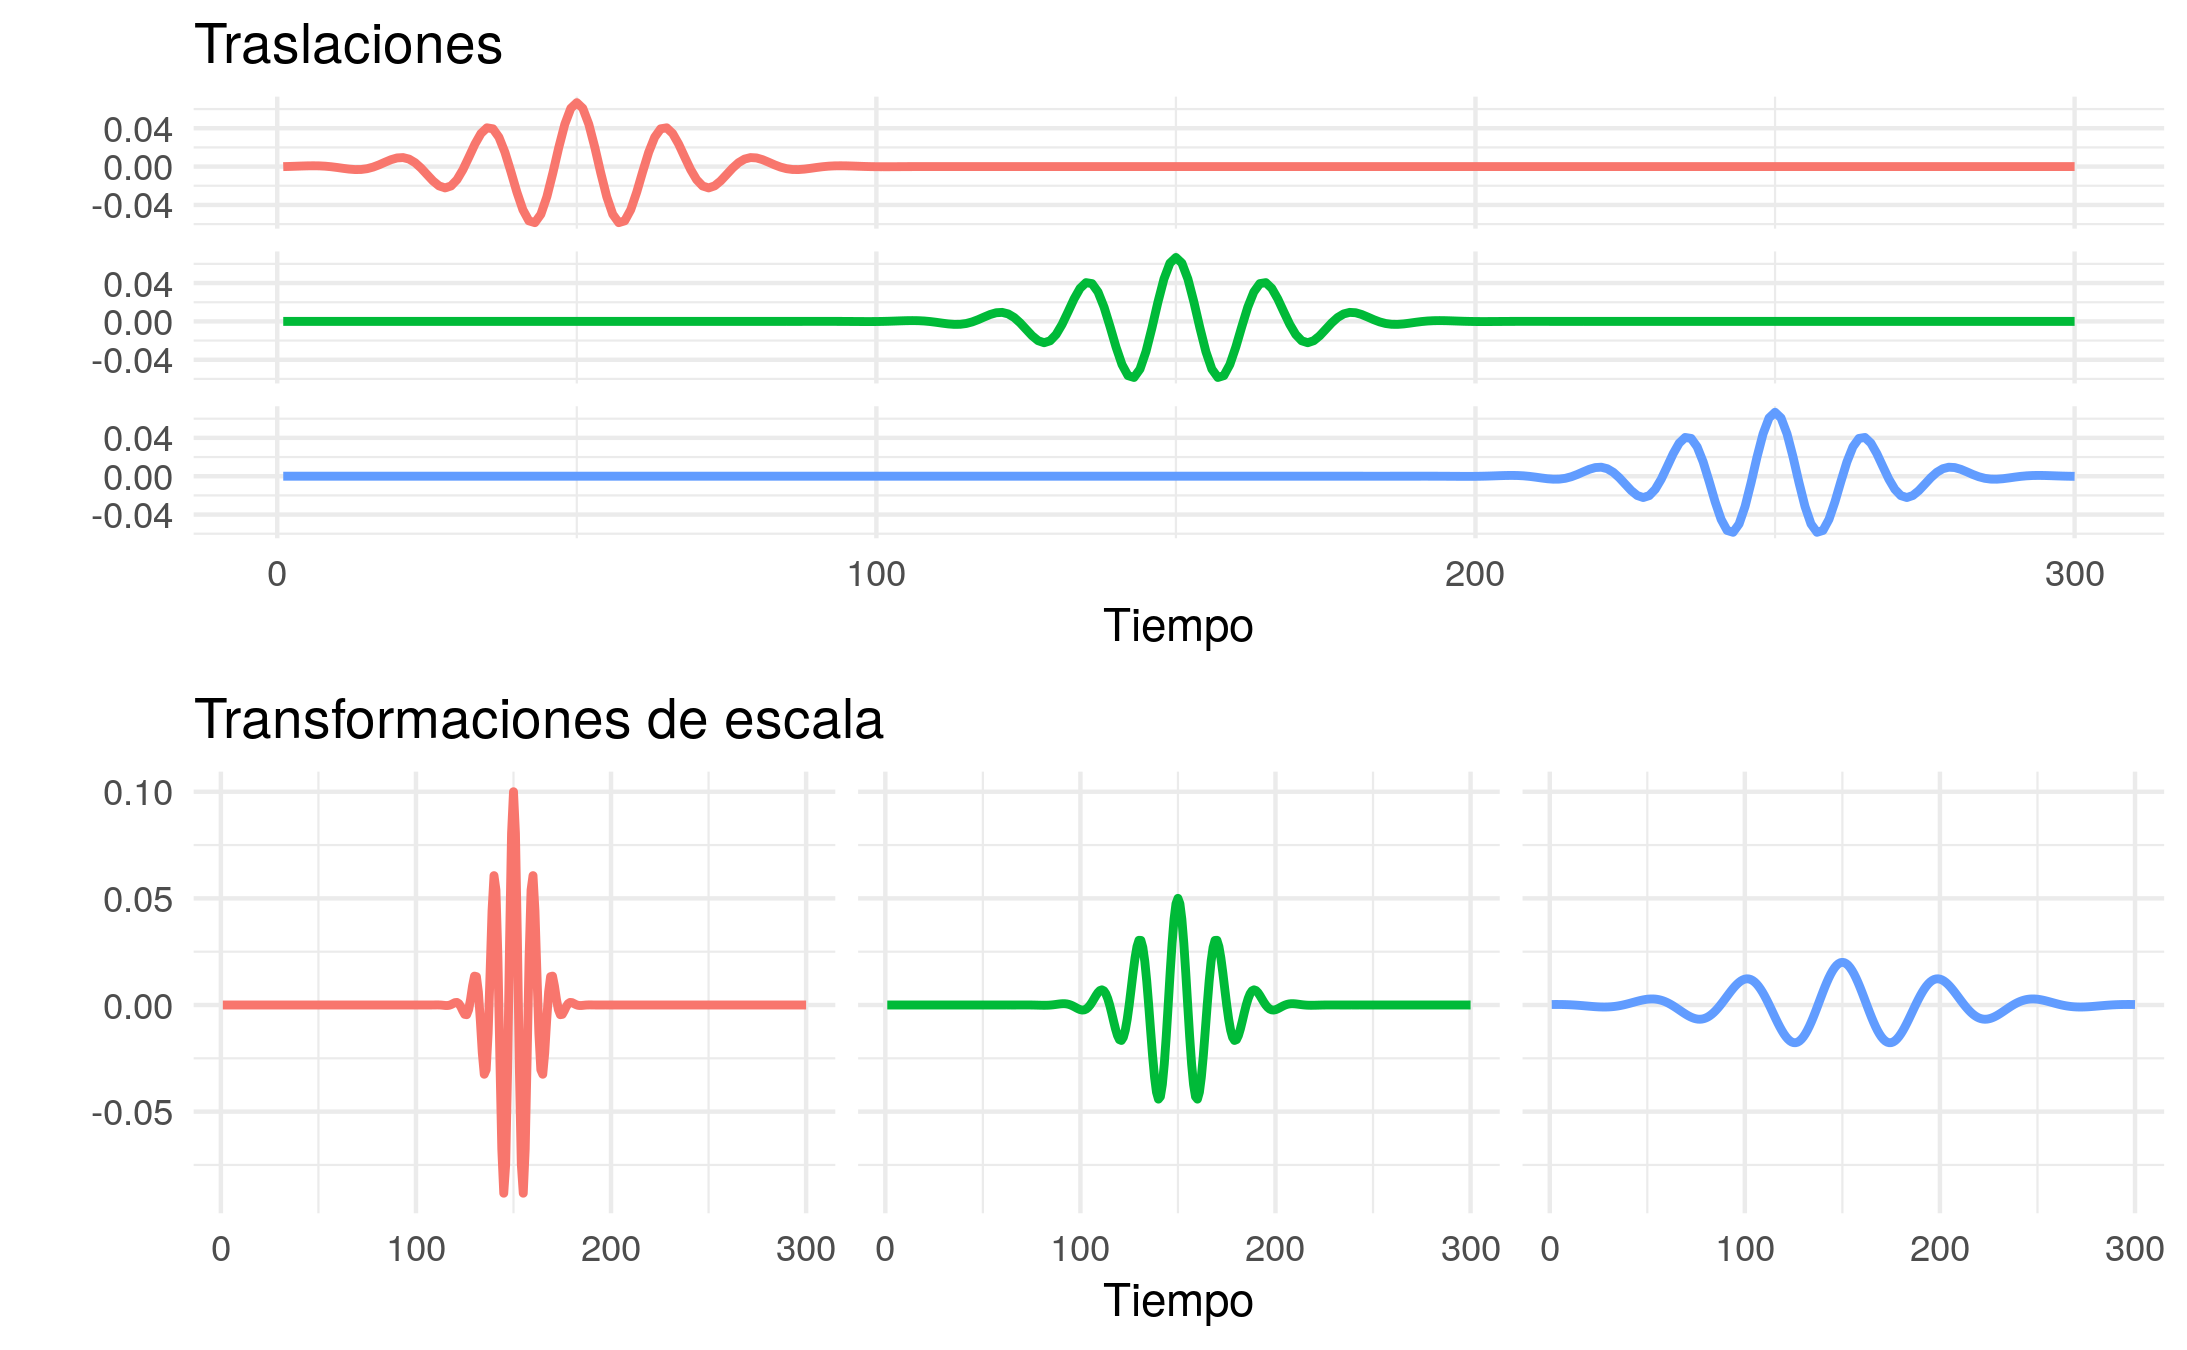
\includegraphics[width=\linewidth]{morelt.png}
	\caption{Traslaciones y reescalados de la función base Morlet} \label{fig:morlet}
\end{figure}

Para visualizar las wavelets en el análisis del ciclo económico es propicio definir un modelo teórico de una economía cíclica, con los diferentes componentes vistos por separado y en su composición, para observar las características del espectograma en este modelo,  y luego compararlo con los datos reales. 
En la figura \ref{fig:serie_teorica} se observan 100 valores de los distintos componentes con los que construiremos la serie, los mismos son:

\begin{itemize}
	\item \textbf{impulso}: Una serie con un valor constante de 50, que en período en particular tomar el valor 100.
	\item \textbf{Tendencia}: Crece medio punto por período.
	\item \textbf{ciclo corto}: Un ciclo de amplitud y extensión pequeña
	\item \textbf{ciclo medio}: Un ciclo de amplitud y extensión media
	\item \textbf{ciclo largo}: Un ciclo de amplitud y extensión grande
	\item \textbf{ruido}: Ruido generado a partir de una distribución normal, poco significativo respecto a la amplitud de los ciclos y la pendiente de la tendencia.
\end{itemize}

En código R, los elementos de la serie teórica se pueden expresar de la siguiente manera:

\begin{lstlisting}
n = 1000
impulso= c(rep(50,(n/2-1)),100,rep(50,n/2))
tendencia = c(1:n)/2
corto = 10 * sin(( 2 * pi/3 ) * c(1:n))
medio = 20 * sin(( 2 * pi/10) * c(1:n))
largo = 30 * sin(( 2 * pi/50) * c(1:n))
ruido <- rnorm(n)
serie_compuesta = impulso + tendencia + corto + medio + largo + ruido
\end{lstlisting}


\begin{figure}[H]
	\centering
	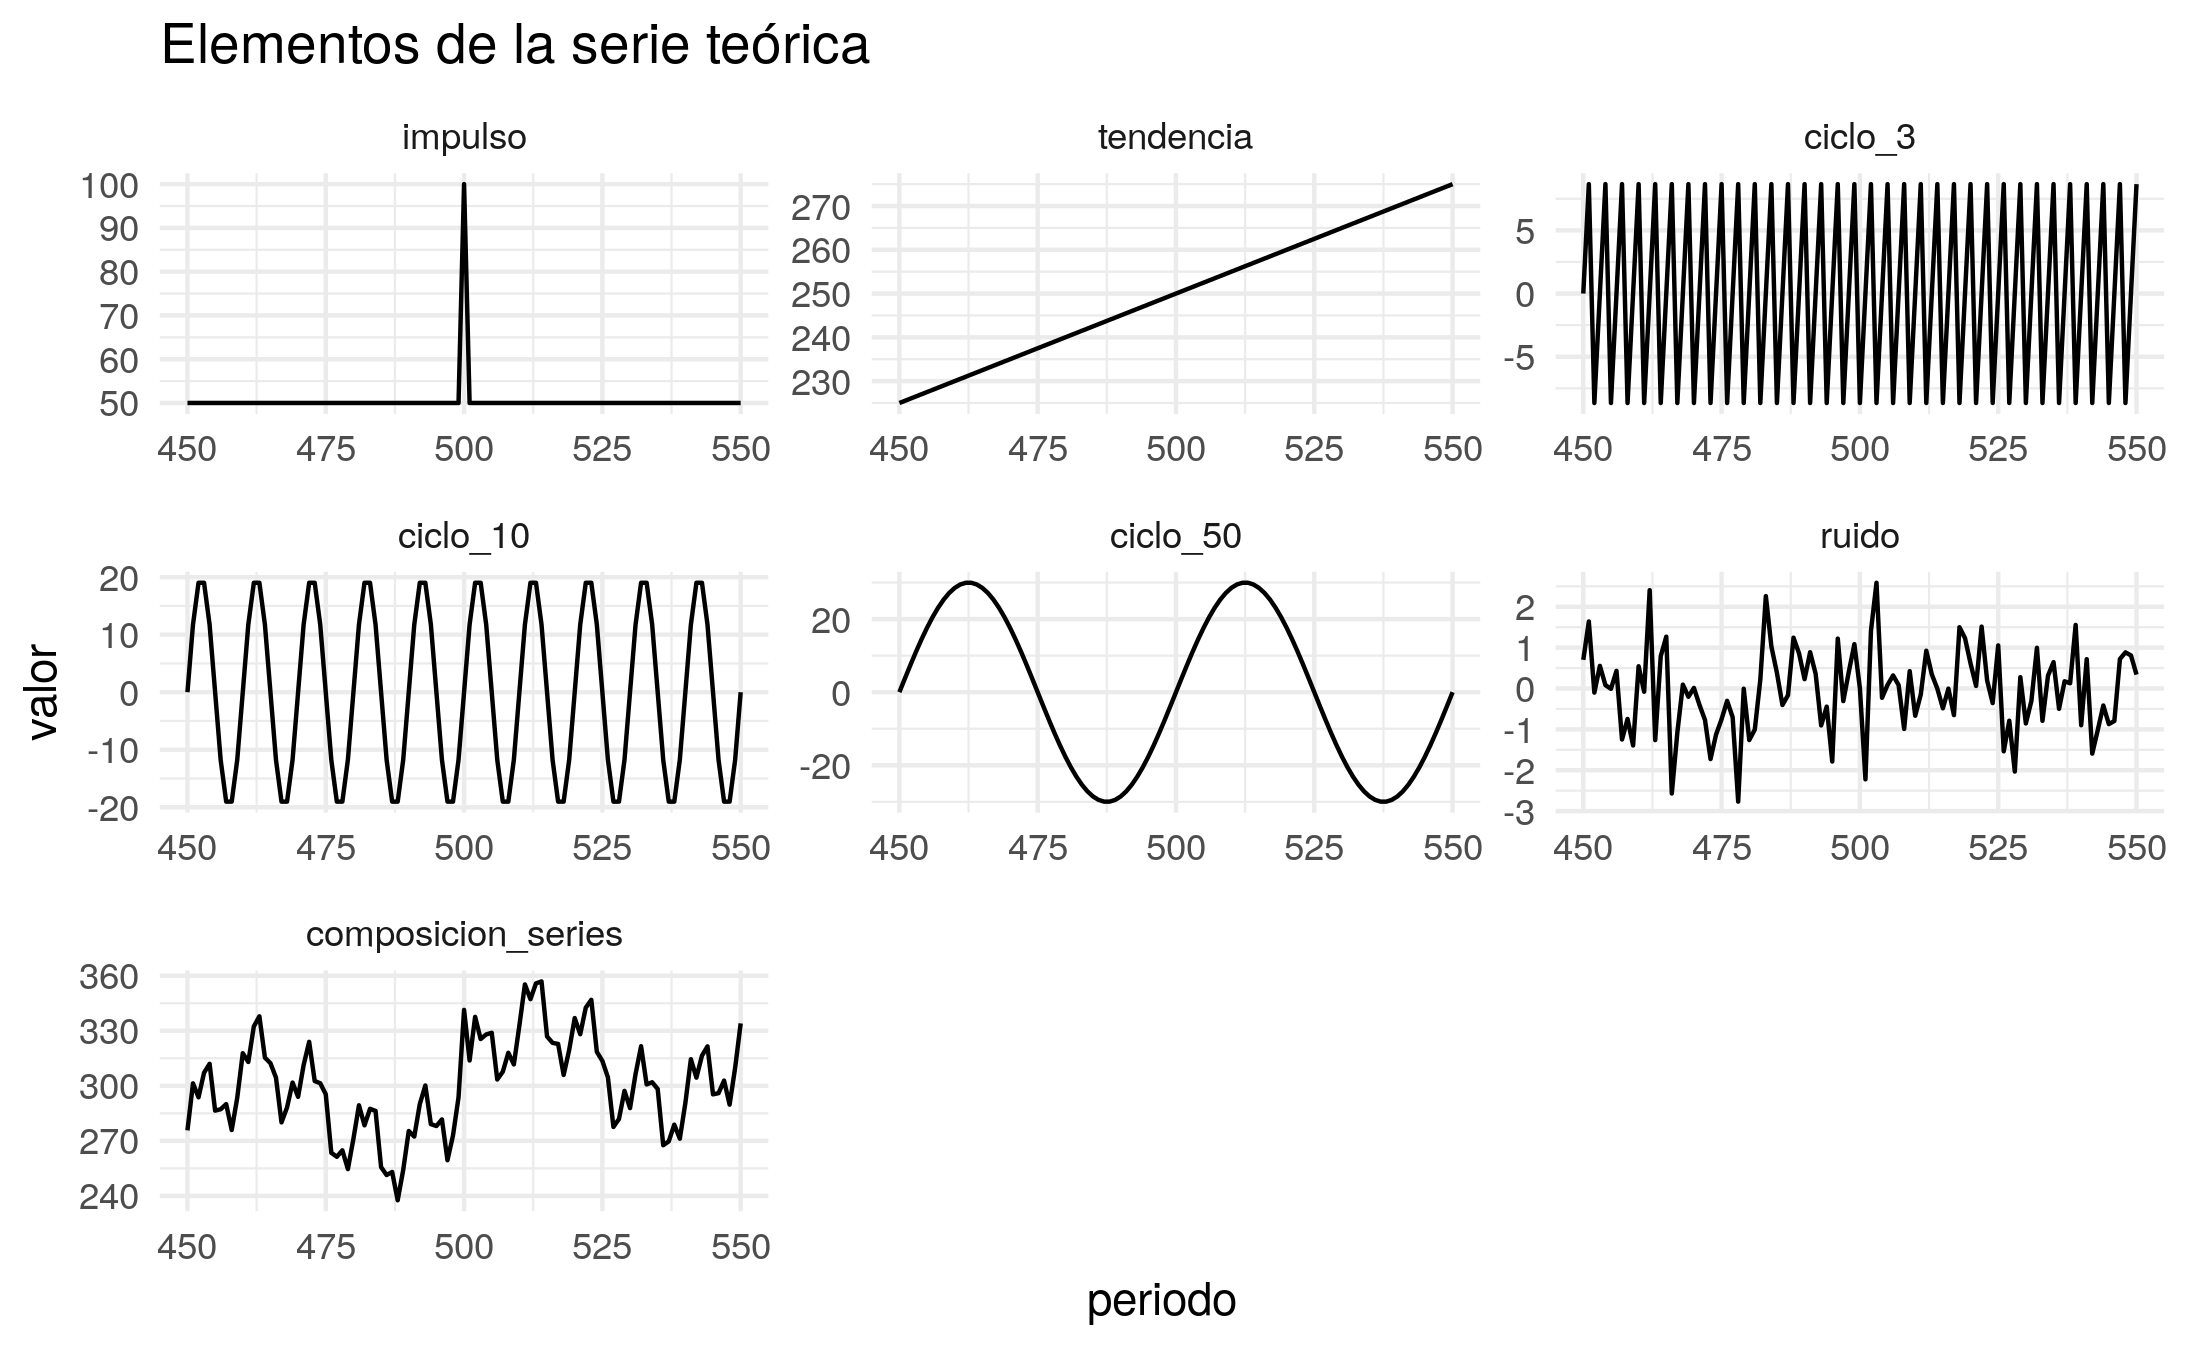
\includegraphics[width=\linewidth]{serie_teorica.PNG}
	\caption{Serie Teórica} \label{fig:serie_teorica}
\end{figure}

En la figura \ref{fig:espect_teo} se observa el espectograma de cada uno de los elementos mencionados. Dicho gráfico muestra en el eje vertical el período, la inversa de la frecuencia de onda, que corresponde a la distancia entre los valles o picos de un ciclo. La escala cromática (de los azules para los valores más bajos a los rojos en los valores más altos) representa la amplitud del ciclo. el eje horizontal representa el tiempo calendario. Es decir, para cada tiempo calendario podemos observar la amplitud del ciclo en cada una de las posibles frecuencias de onda. 

\begin{figure}[H]
	\centering
	\subfigure[impulso]{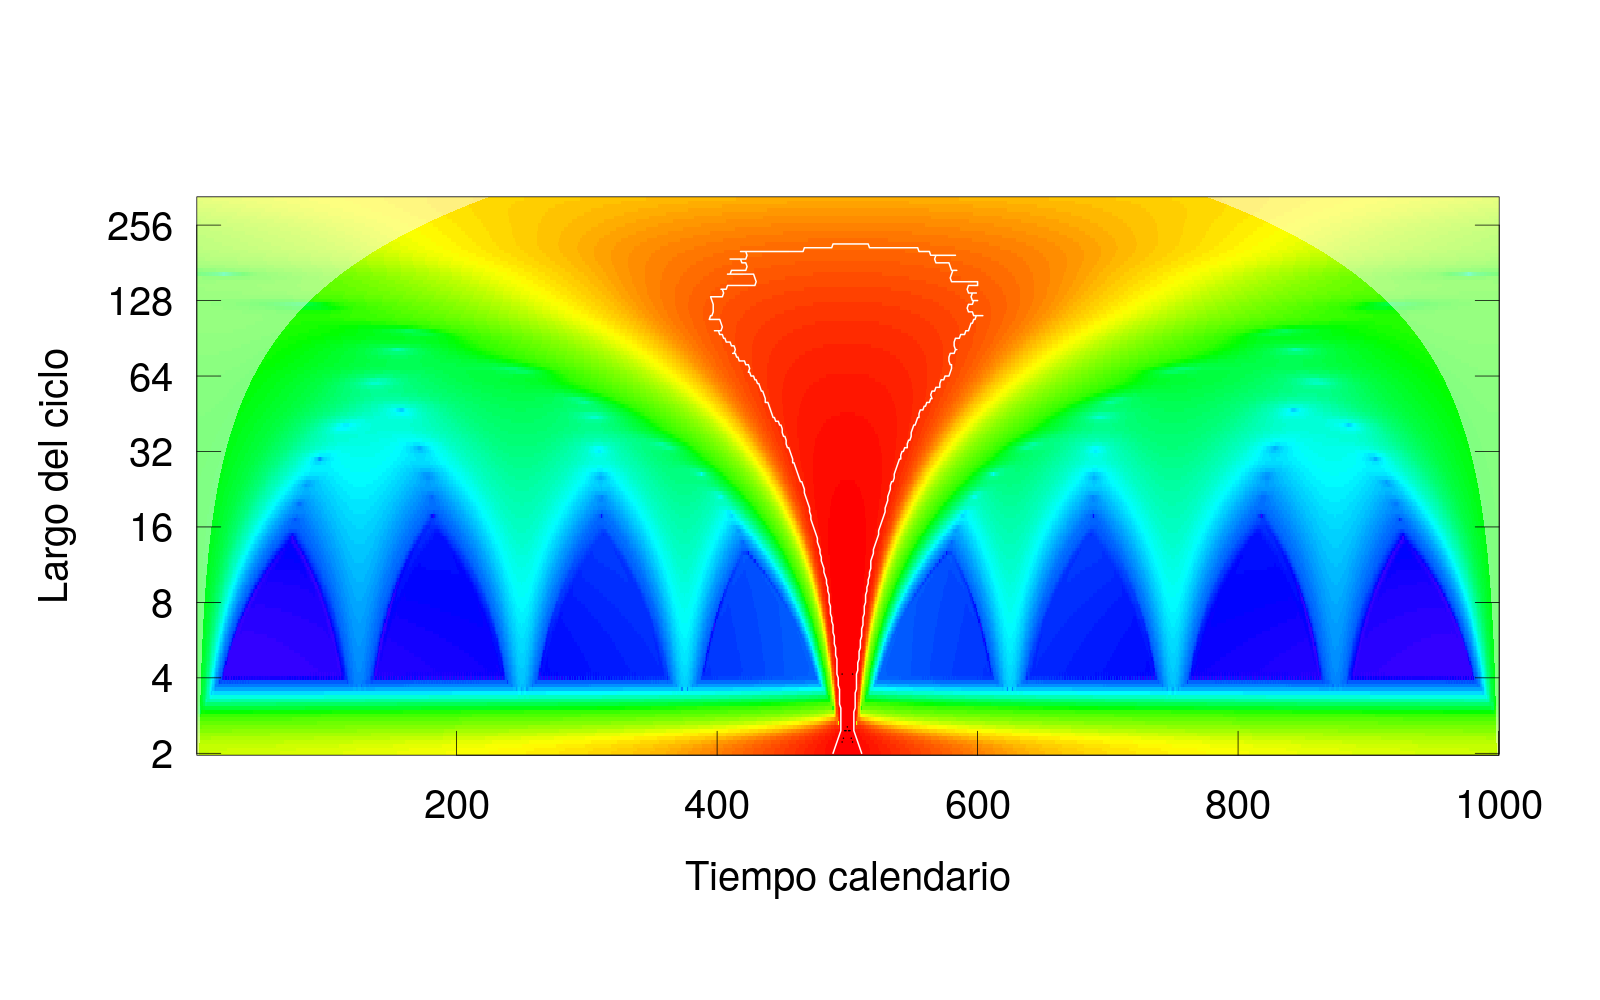
\includegraphics[width=0.49\linewidth]{espectograma_teorico_impulso.png}}
	    \vspace{0.00mm}
	\subfigure[tendencia]{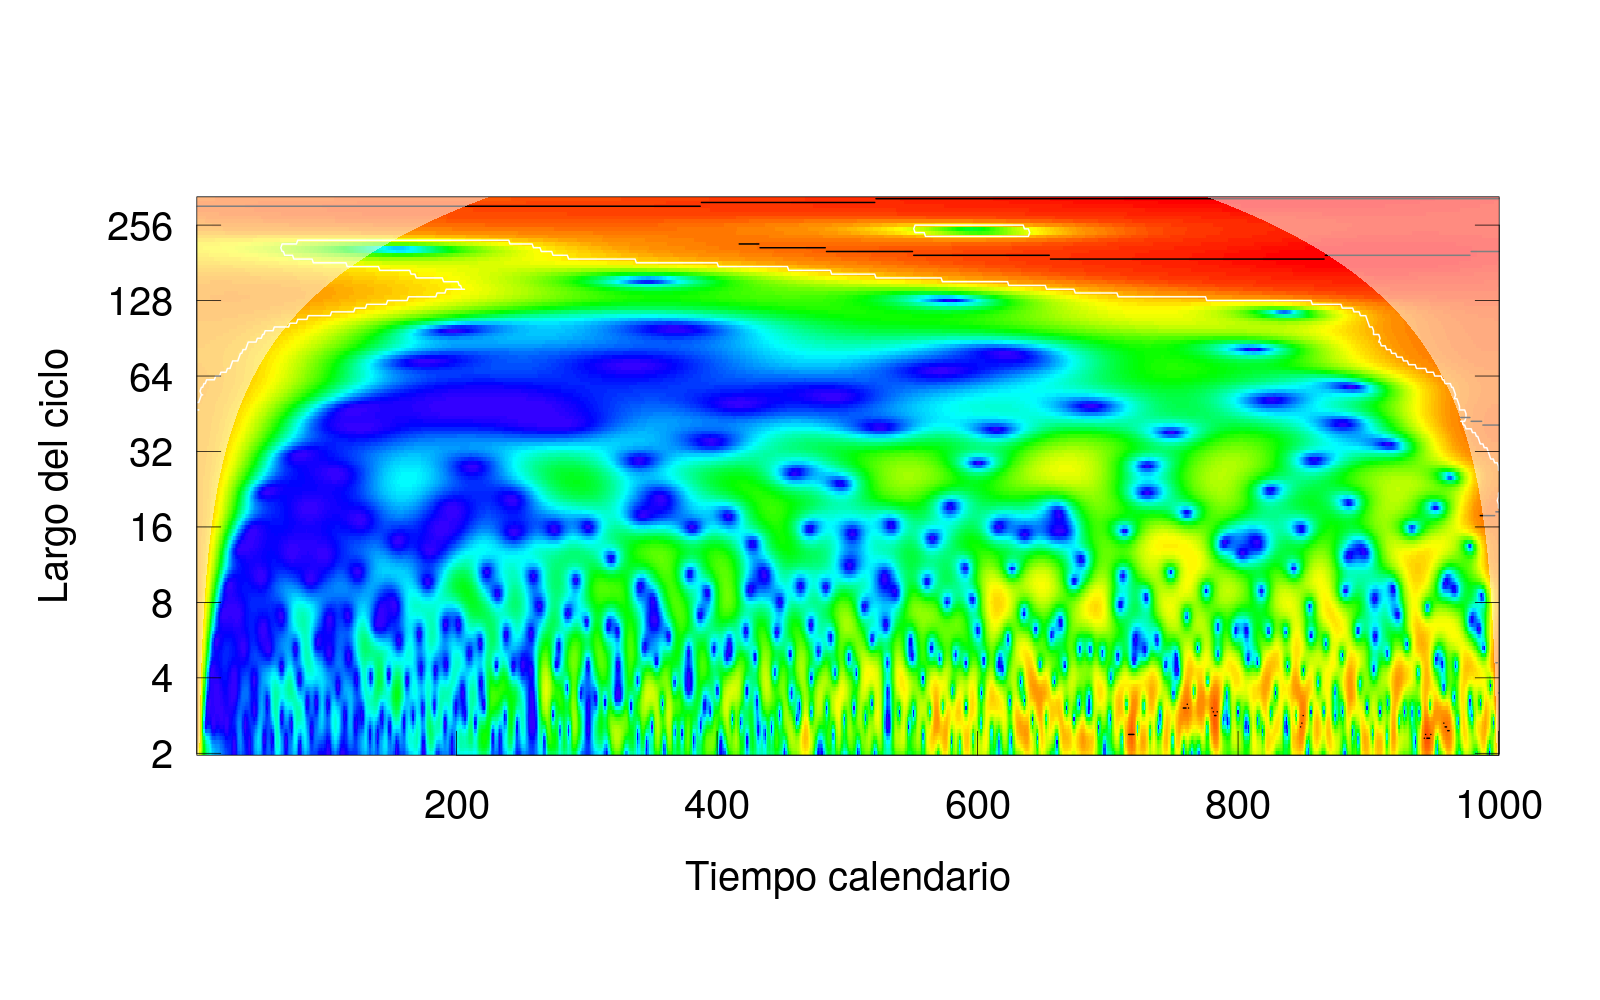
\includegraphics[width=0.49\linewidth]{espectograma_teorico_tendencia.png}}
	    \vspace{0.00mm}
	\subfigure[ciclo de 3 años]{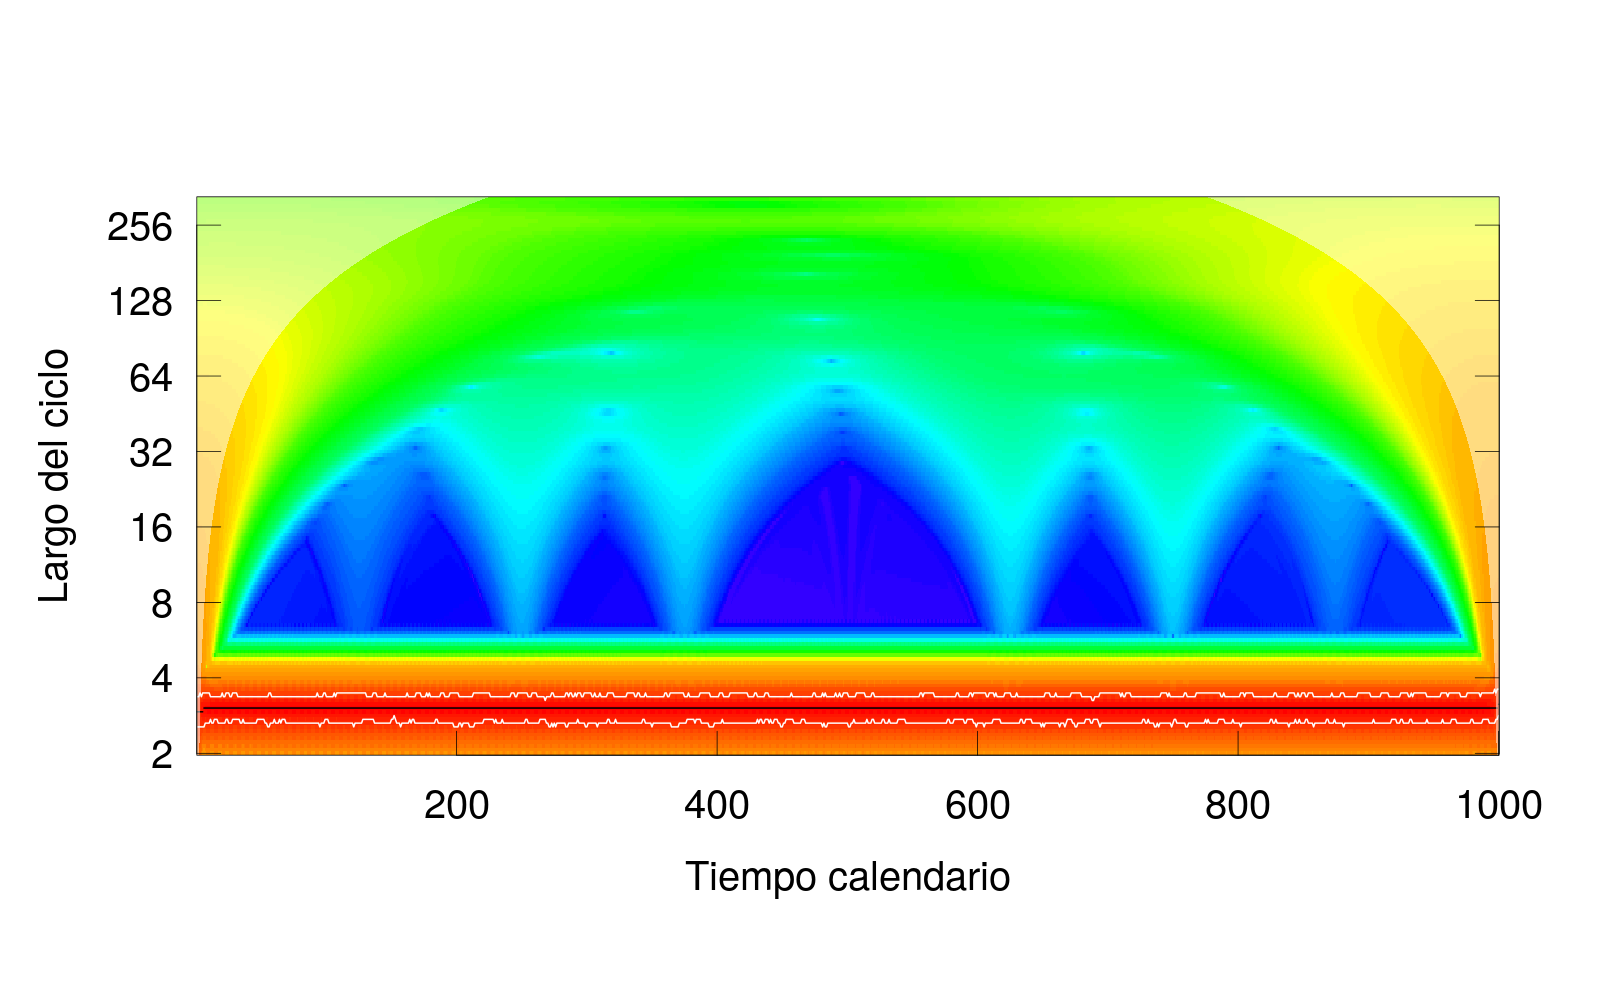
\includegraphics[width=0.49\linewidth]{espectograma_teorico_ciclo_3.png}}
	    \vspace{0.00mm}
	\subfigure[ciclo de 10 años]{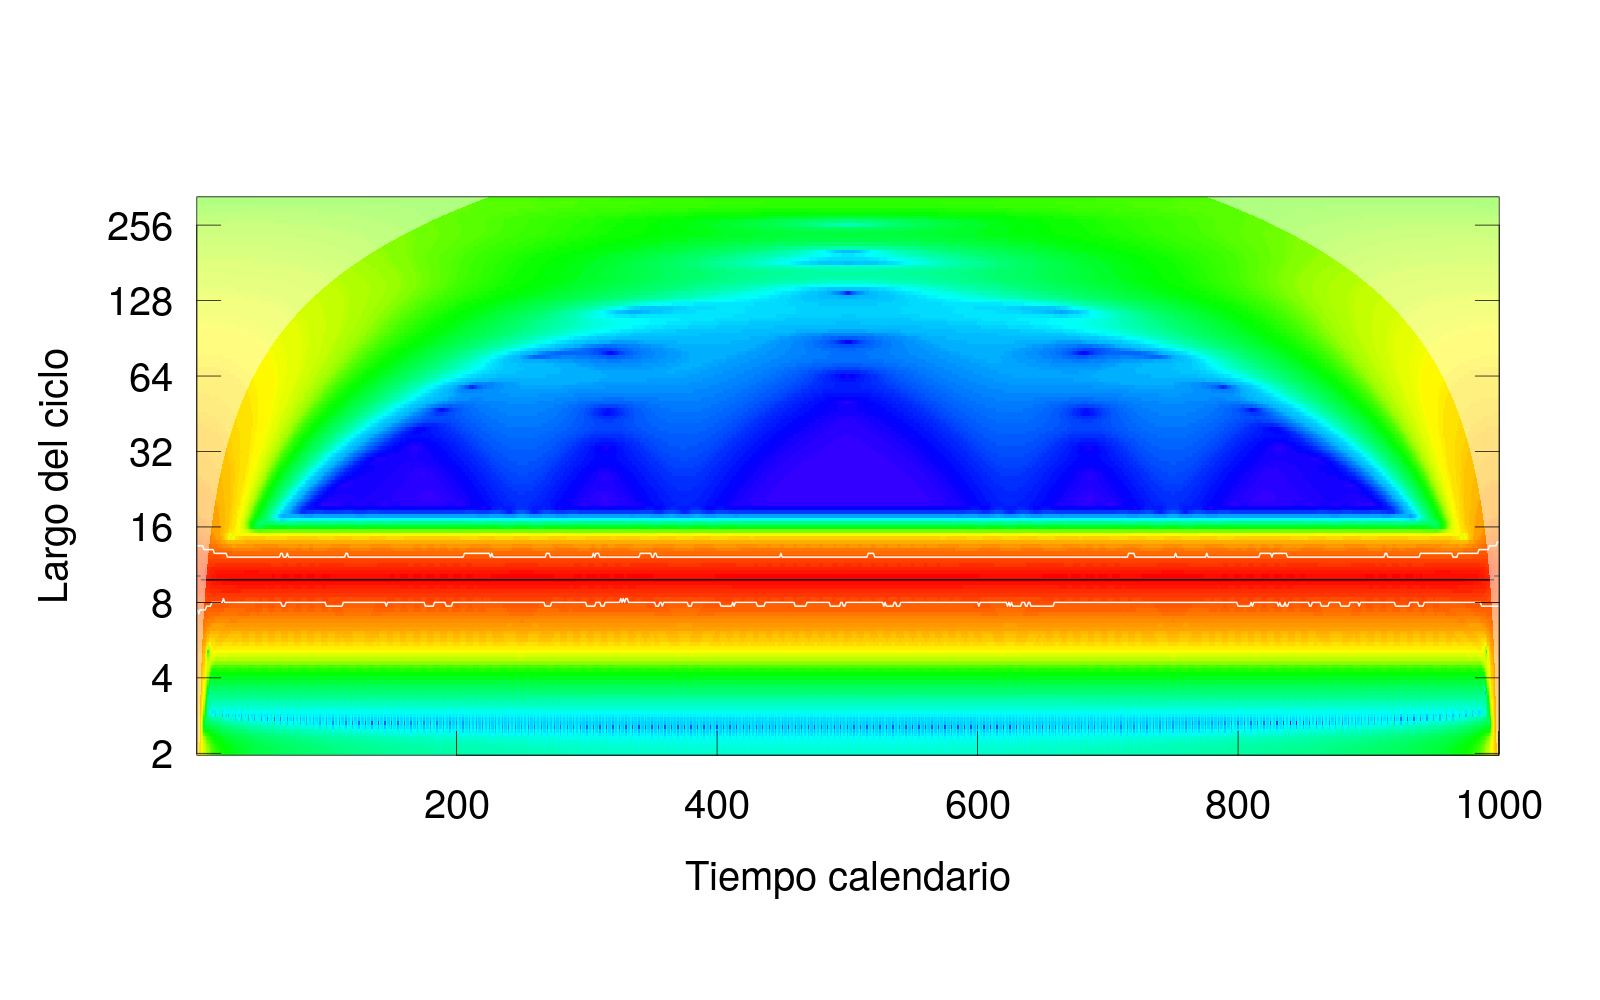
\includegraphics[width=0.49\linewidth]{espectograma_teorico_ciclo_10.png}}
	    \vspace{0.00mm}
	\subfigure[ciclo de 50 años]{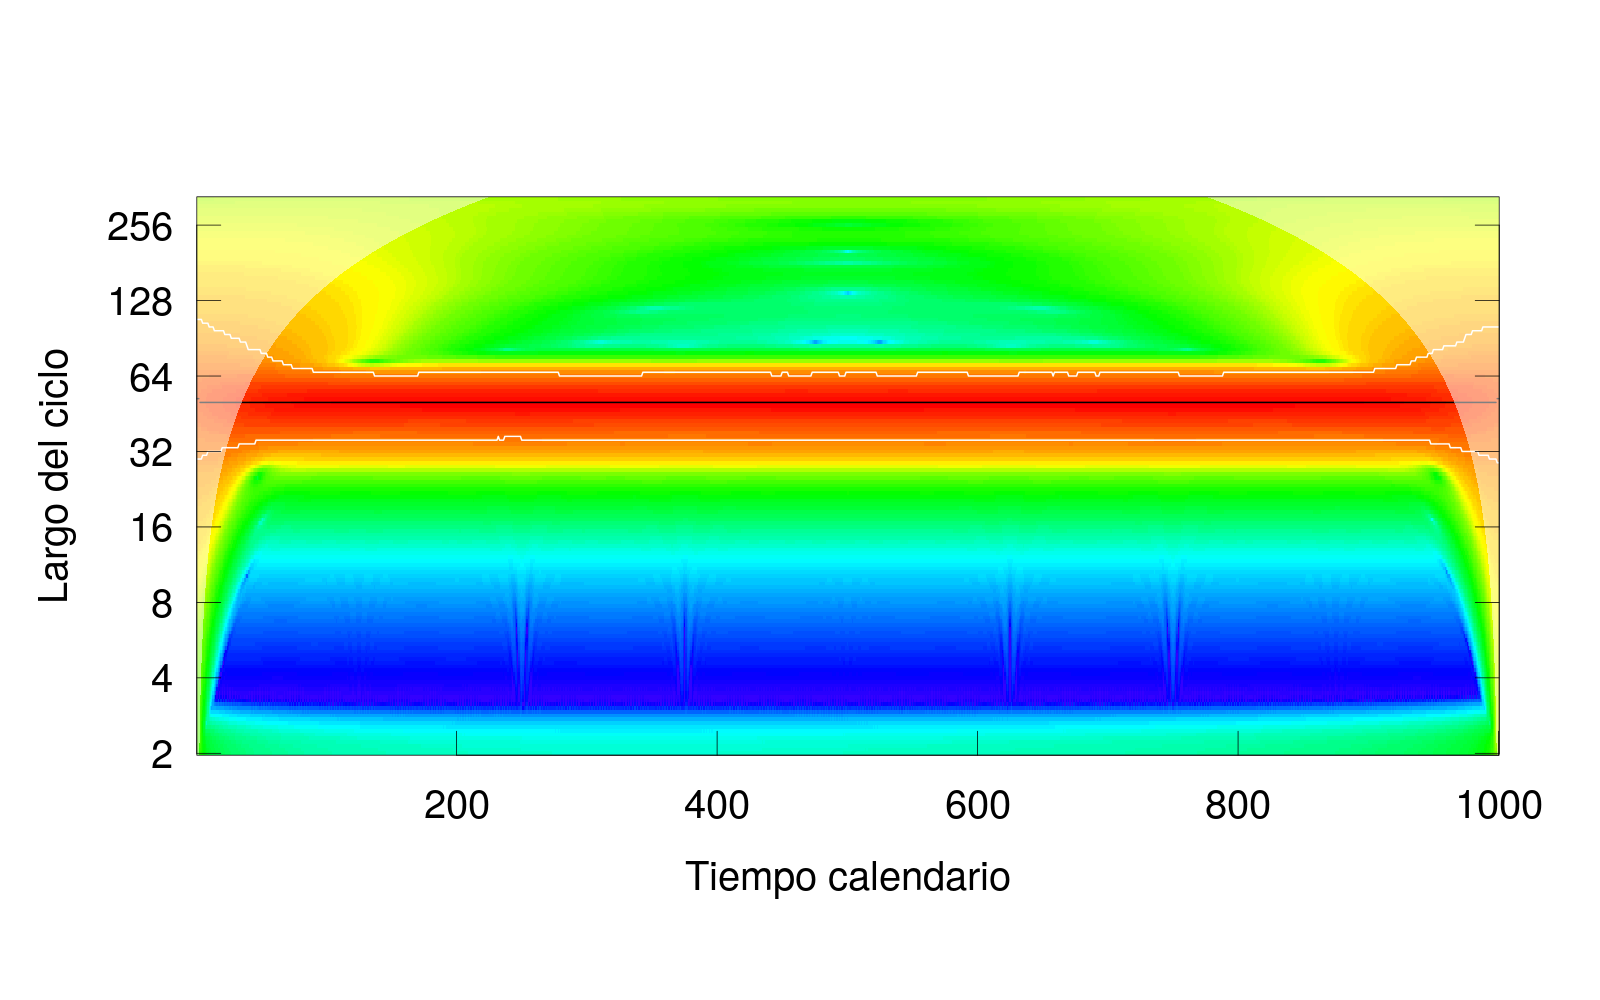
\includegraphics[width=0.49\linewidth]{espectograma_teorico_ciclo_50.png}}
	    \vspace{0.00mm}
	\subfigure[ruido normal]{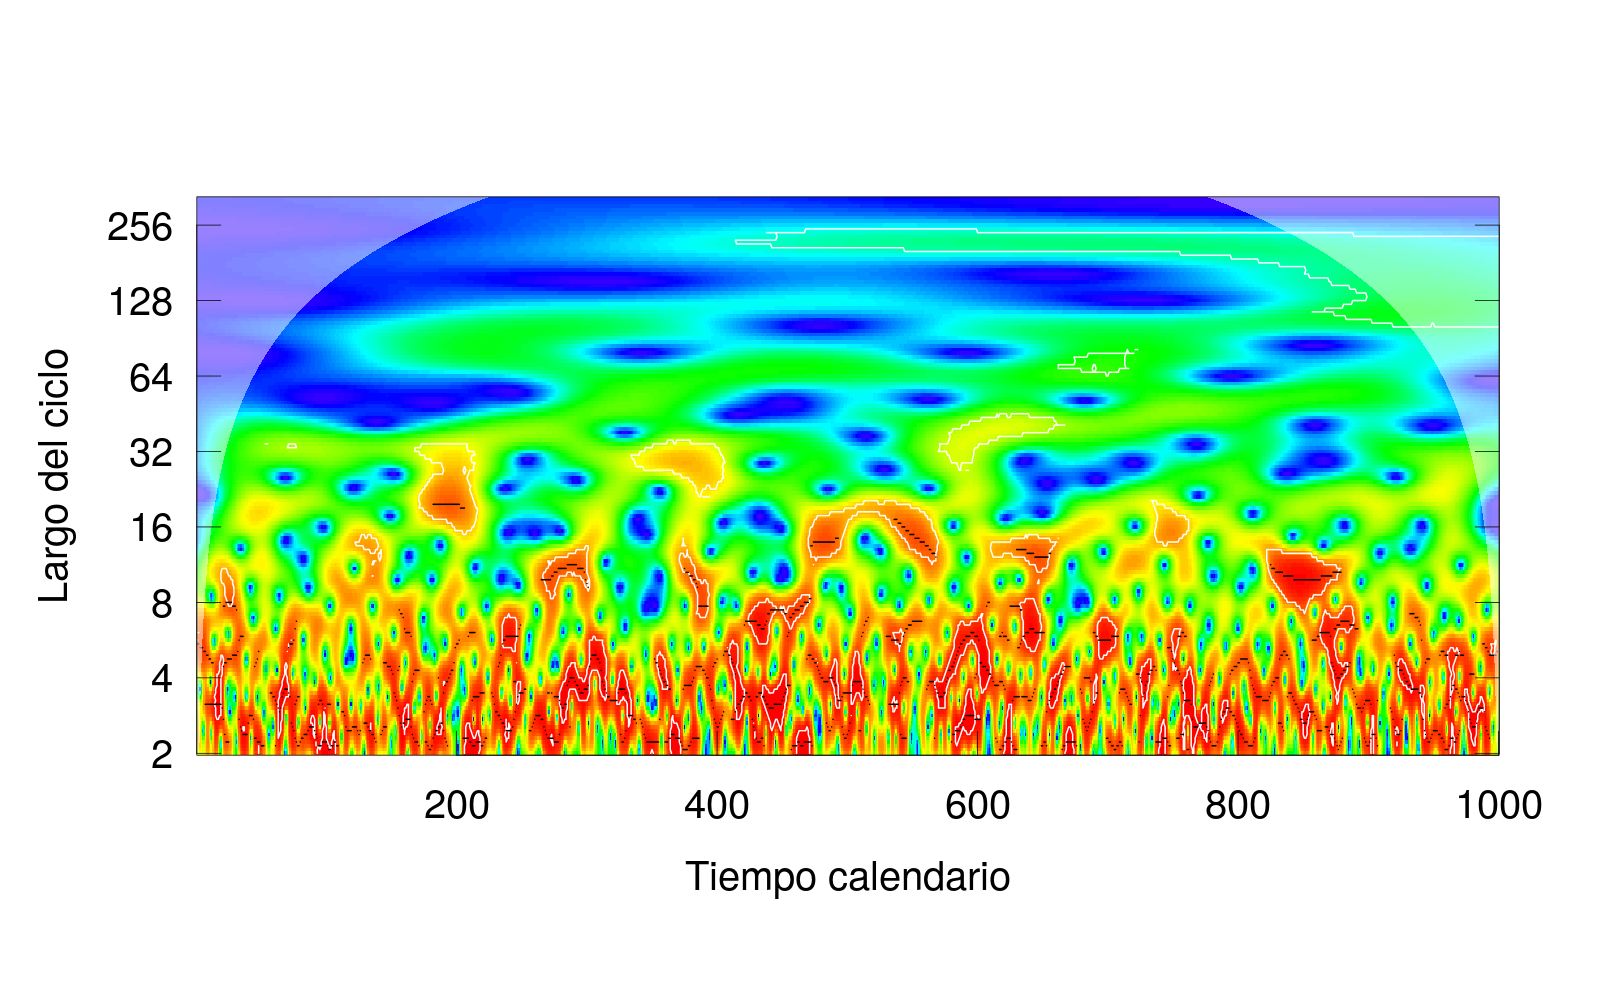
\includegraphics[width=0.49\linewidth]{espectograma_teorico_ruido.png}}
	    \vspace{0.00mm}
	\subfigure[composición de series]{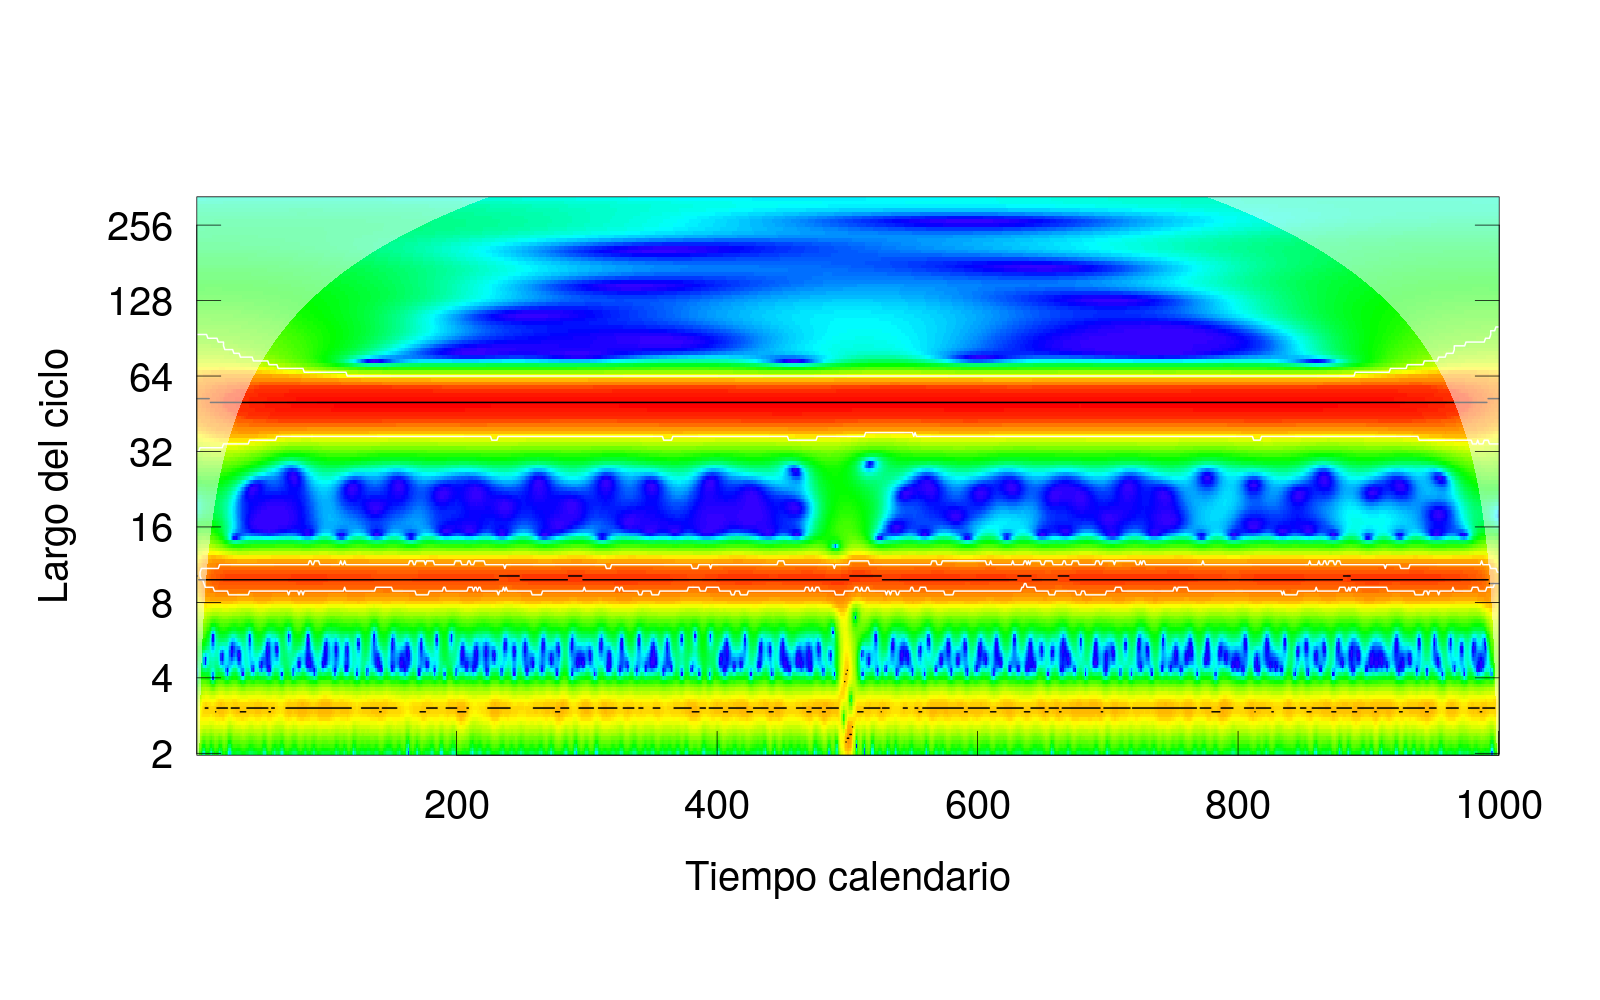
\includegraphics[width=0.75\linewidth]{espectograma_teorico_composicion_series.png}}
	\caption{Espectogramas Teóricos} \label{fig:espect_teo}
\end{figure}

Como se observa en la figura \ref{fig:espect_teo} el impulso se presenta como un ciclo de amplitud grande en todas las frecuencias, en el momento correspondiente. La tendencia, por su parte, se presenta básicamente como ruido, dado que es estrictamente un comportamiento no cíclico. Sin embargo, presenta la particularidad de presentar valores de amplitud mayores hacia el final del período para frecuencias bajas, y valores de amplitud particularmente bajos en las frecuencias altas de los primeros momentos.

Los tres ciclos definidos marcan claramente una línea horizontal en el correspondiente período, que luego se diluye hacia las demás frecuencias. Finalmente, el ruido normal presenta un comportamiento muy particular, mostrando mayores amplitudes, de forma irregular, en las frecuencias altas, y homogeneizándose hacia un valor de amplitud baja en los ciclos más largos. Esto se debe a que el ruido normal se puede parecer a un ciclo de períodos muy cortos debido a una sucesión de subas y bajas, pero dado que es un proceso aleatorio, es cada vez más improbable que se asemeje a ciclos de períodos mayores, dado que ello implicaría una mayor cantidad de sucesiones de subas y bajas consecutivas. A su vez, tanto en el espectograma del ruido normal como en el de la tendencia se puede apreciar como el gráfico pierde resolución para periodos más largos, como se mencionó anteriormente. 

Por último, en la composición se series se observa como los ciclos de mayor amplitud y frecuencia se expresan en la escala cromática de forma más nítida que los ciclos de menor amplitud y frecuencia. Es importante resaltar que la concordancia entre amplitud y frecuencia es producto de la forma en que construimos las series, dado que esperamos que los ciclos económicos más largos se correspondan también con movimientos de mayor amplitud.

Vale mencionar que la elección para el modelo teórico de estos tres niveles y amplitudes cíclicas no es arbitraria, sino que se corresponde a grandes rasgos con lo considerado por la literatura: \cite{kondratieff1979long} estudia las series largas, de unos 50 años, mientras que \cite{kuznets1930secular} propone movimientos seculares de entre 15 y 25 años. Finalmente el Real business cycle \citep{kydland1982time} considera un ciclo corto.



Con lo analizado de la figura \ref{fig:espect_teo} podemos observar los resultados de las series originales. En la figura \ref{fig:espect_PBI_a} se puede observar el espectograma correspondiente al PBI de Estados Unidos expresado en oro. Allí se marca claramente la diferencia en la serie antes y después del 1900, y en particular también se marca el quiebre estudiado de los años 70'. No obstante lo cual, para ese período se observan 3 frecuencias donde se registra un comportamiento cíclico, en los períodos aproximados de 8 y 50 años, y un ciclo diferenciado de este último, de aproximadamente 30 años. Dada la heterocedasticidad de las series, en \ref{fig:espect_PBI_b} se propone el espectograma de la misma serie tomada en logaritmo de base 10. De esta forma lo que se observa es que el ciclo de 50 años se extiende más allá en el tiempo, hasta mediados del Siglo XIX. Por su parte, aparece brevemente un ciclo más corto, de aproximadamente tres años, en la década del 70.

\begin{figure}[H]
	\centering
	\subfigure[PBI]{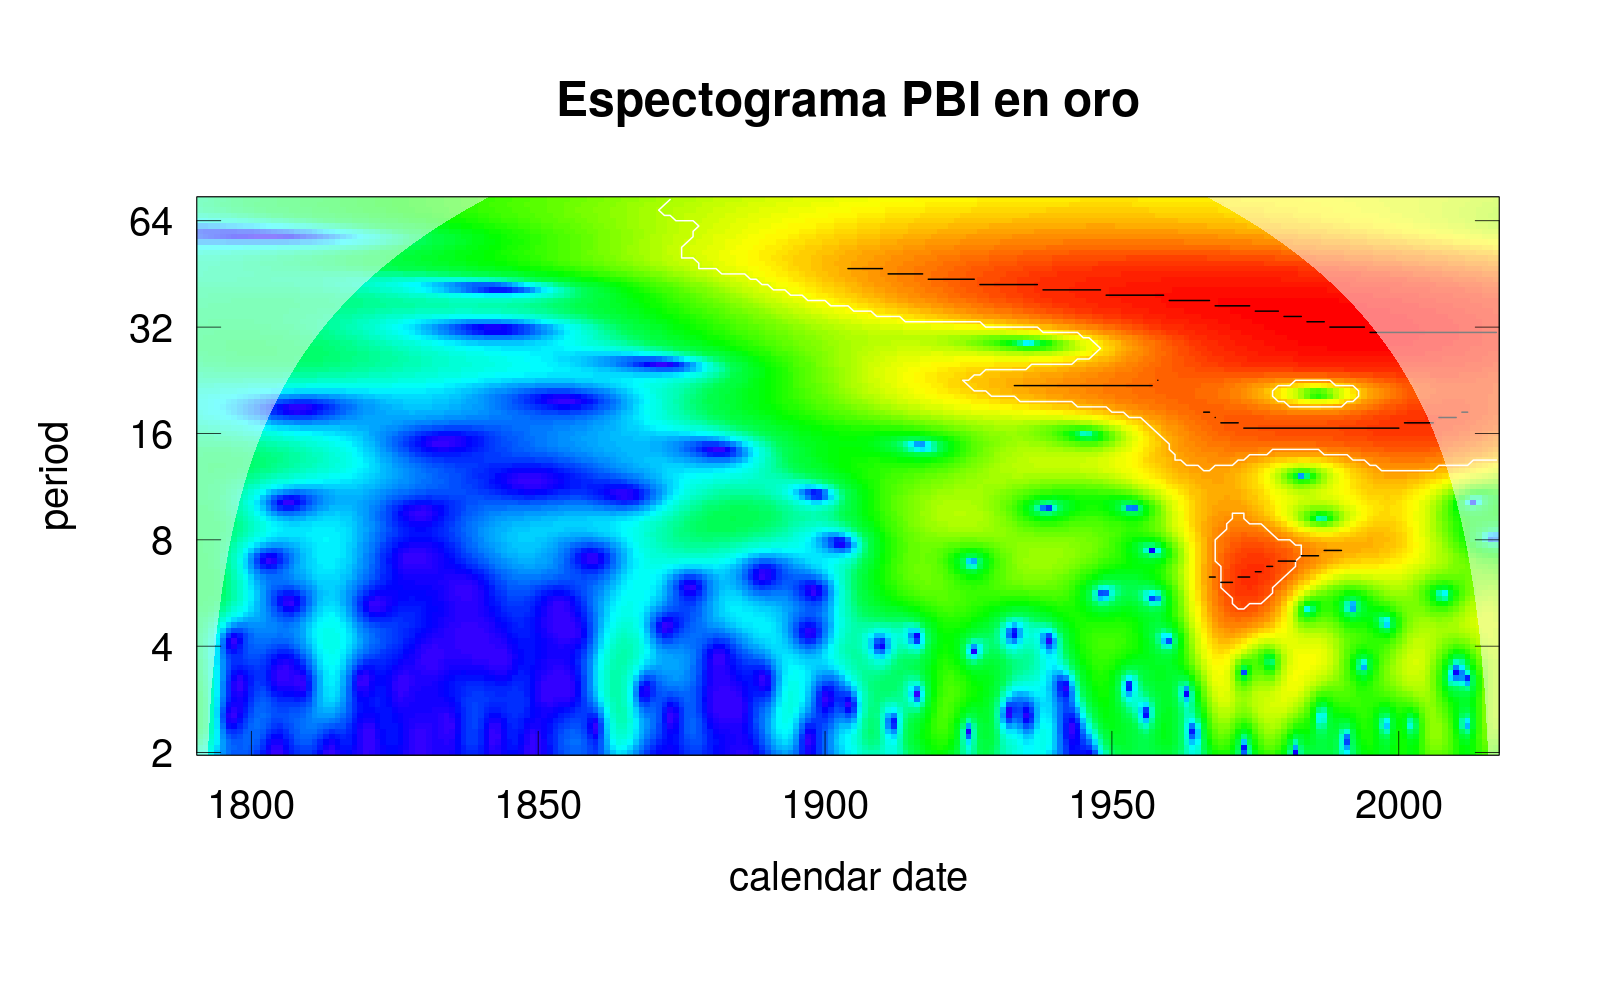
\includegraphics[width=0.75\linewidth]{espectograma_gdp.png}
	\label{fig:espect_PBI_a}}
	\subfigure[$log(PBI)$]{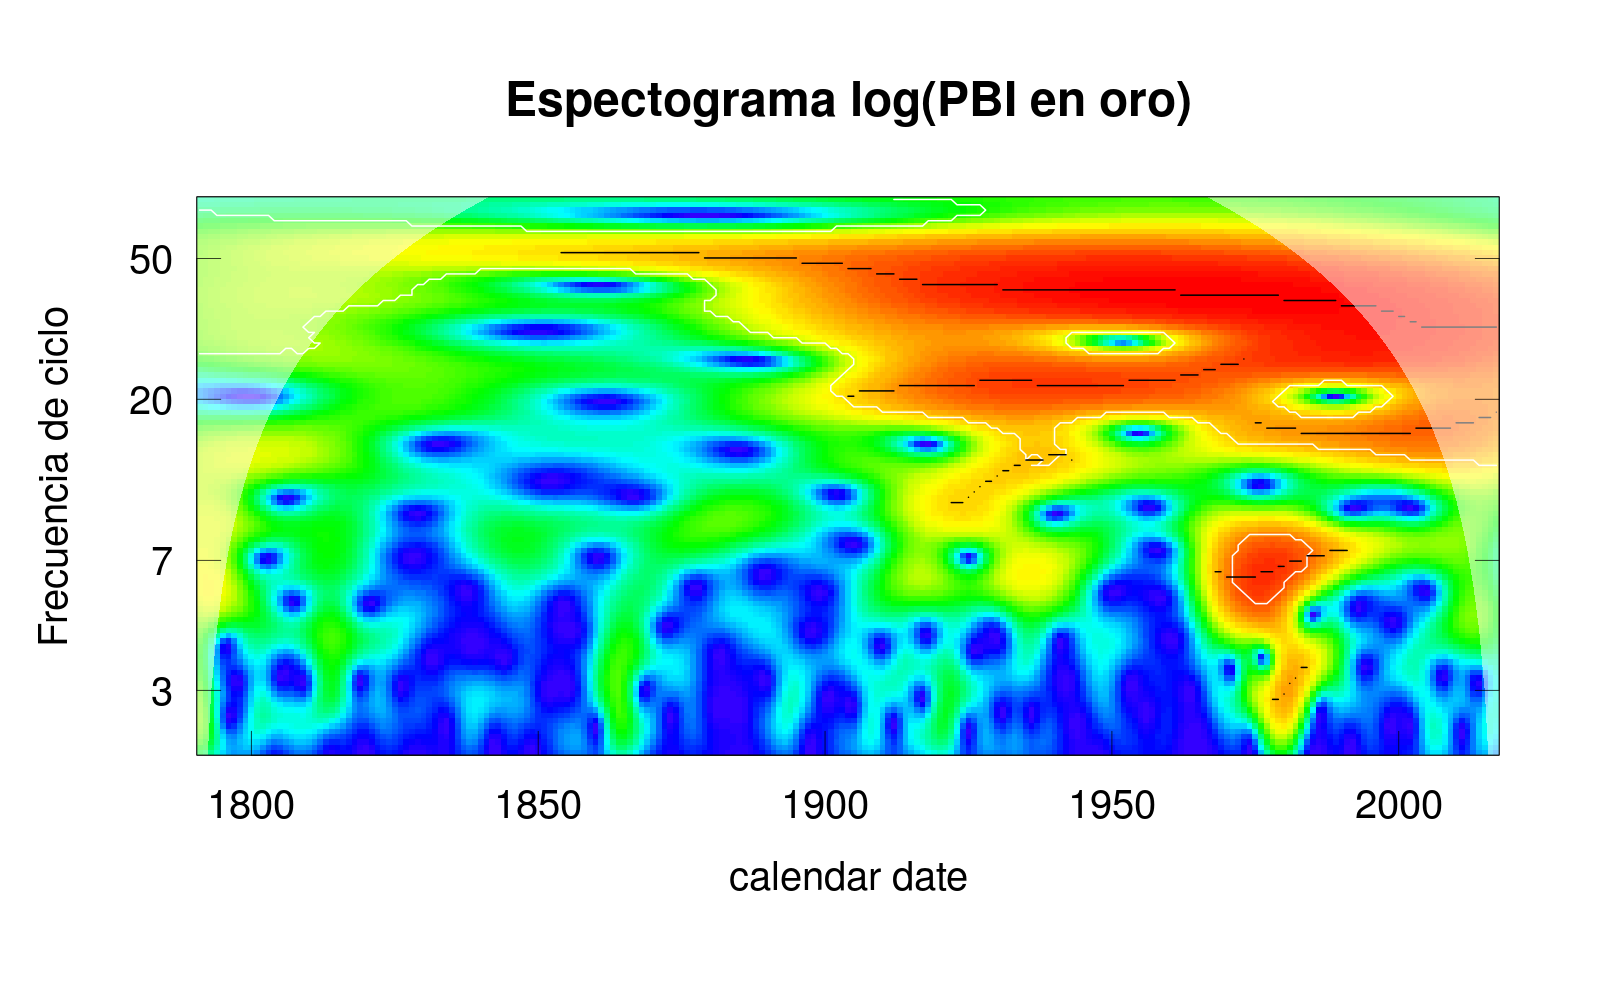
\includegraphics[width=0.75\linewidth]{espectograma_log_gdp.png}
	\label{fig:espect_PBI_b}}
	\caption{Espectograma PBI en oro} \label{fig:espect_PBI}
\end{figure}

las figuras \ref{fig:espect_wg} muestran los espectogramas de la serie del salario expresado en oro \ref{fig:espect_wg_a} y el mismo tomado en logaritmo en \ref{fig:espect_wg_b}. Para esta serie nuevamente se observa un ciclo largo bien definido en torno a los 50 años, especialmente si se observa la serie tomada en base logarítmica. Este ciclo largo parece oscilar entre las frecuencias de $1/32$ y $1/64$, cayendo en el tiempo. Por su parte, se delimita un segundo ciclo, en torno a los 16 años de extensión, y finalmente un ciclo corto de entre 6 y 8 años.  Al tomar la escala logarítmica, también aparece un ciclo de mayor frecuencia, de unos 3 años de duración. En consecuencia, ambas series parecen arrojar resultados en concordancia, sean o no tomadas en logaritmo. 

\begin{figure}[H]
	\centering
	\subfigure[Salario]{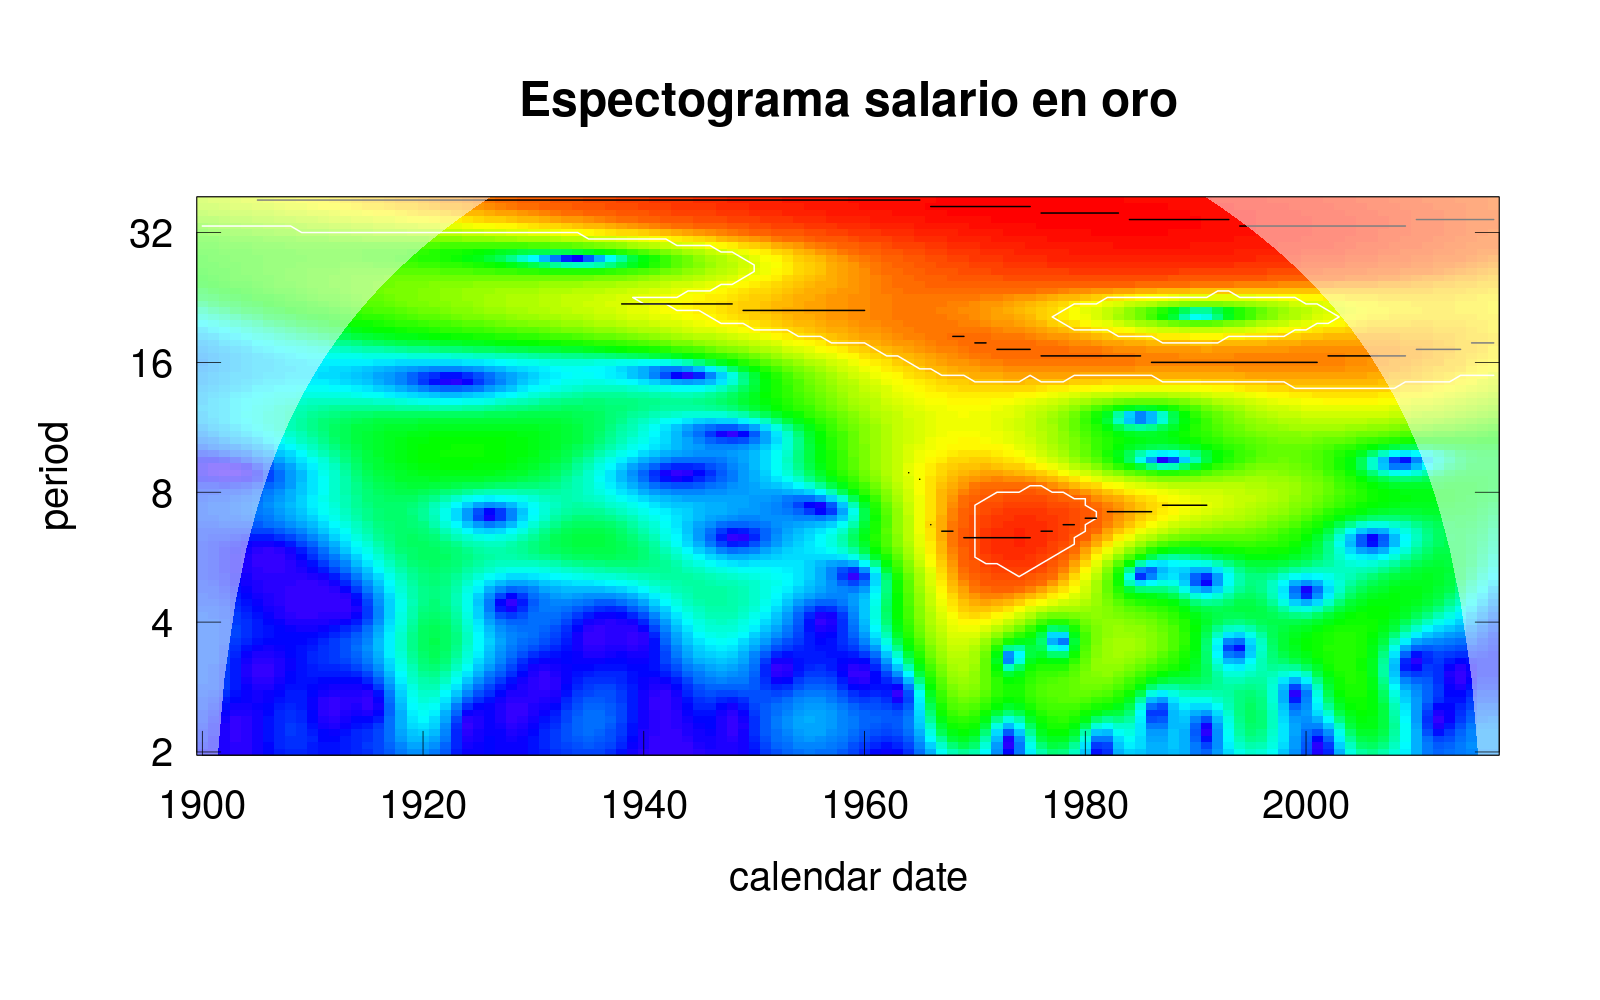
\includegraphics[width=0.75\linewidth]{espectograma_wg.png}
	\label{fig:espect_wg_a}}
	\subfigure[$log(Salario)$]{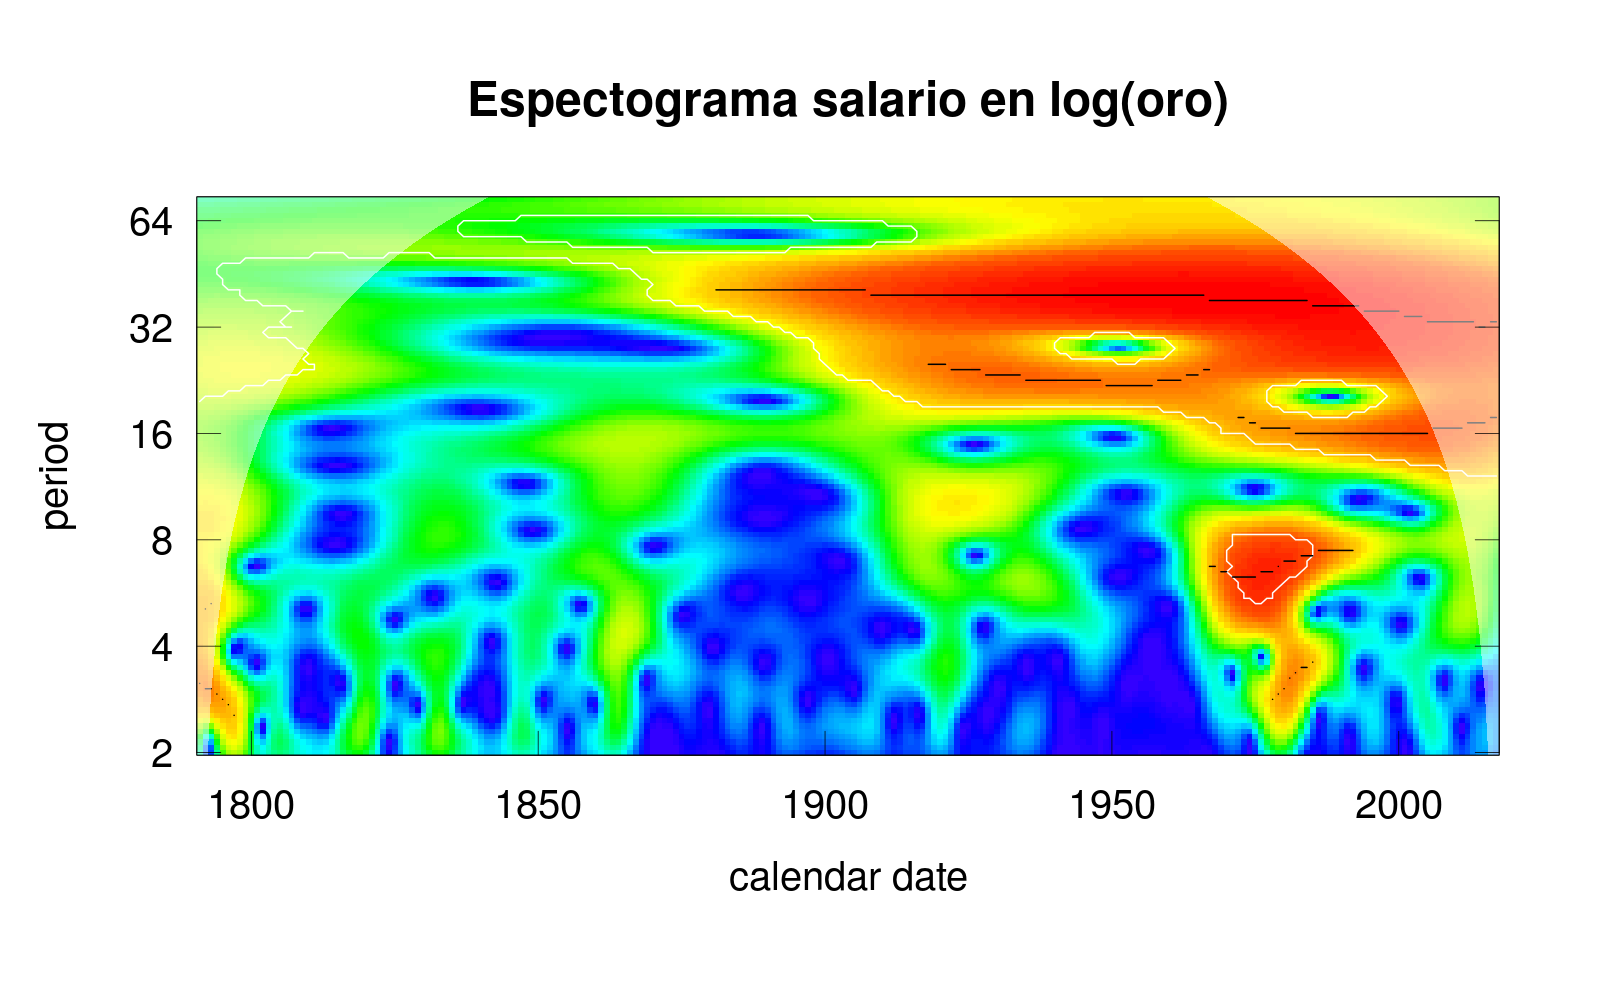
\includegraphics[width=0.75\linewidth]{espectograma_log_wg.png}
	\label{fig:espect_wg_b}}
	\caption{Espectograma Salario en oro} \label{fig:espect_wg}
\end{figure}



\section{Conclusiones}

En el presente trabajo se realizó un recorrido por las principales aproximaciones teóricas respecto al ciclo económico, y se planteó la importancia de un análisis empírico respecto a dicho fenómeno. Para ello, se utilizaron las series de PBI y Salario de Estados Unidos entre 1790 y 2017, expresadas en oro, por los efectos distorsivos que podría generar dicha variable. 

En el análisis exploratorio de datos se encontró una fuerte correspondencia entre los quiebres de estas series, y las crisis conocidas por la historiografía económica, así como un movimiento oscilatorio aparente que pareciera corresponderse con las ondas largas de Kondratieff.

Como se pueden observar ciclos en muchas de las variables macroeconómicas se procedió a continuar con un análisis usando transformaciones de Fourier para descubrir frecuencias bajas de gran amplitud como ciclos de largo plazo en dichas variables, pudiendo también observar series de más corto plazo en los residuos de la descomposición de las series por las ondas largas. Allí se demuestra la utilidad de esta técnica como forma de descomponer las series centradas alrededor de tendencias no cíclicas. Como punto particular para avanzar con la investigación es la continuación de la descomposición de los residuos no explicados hallados de la descomposición con ondas más cortas y medir la capacidad de las ondas resultantes para poder explicar las series con alguna medida estadística, como ser la suma de las diferencias al cuadrado de los datos respecto a un modelo nulo y a la serie cíclica hallada	.

Luego se realizó un análisis con las herramientas clásicas de la econometría de series de tiempo, en particular con funciones de autocorrelación y modelos ARIMA, tomando el recaudo de distinguir las series antes y después de la caída del patrón oro en 1971. Allí se encontró que la variabilidad de la serie luego de este punto es sustancialmente mayor, y presenta esencialmente un comportamiento de tipo \textit{random walk}. Sin embargo, no se consiguió evidencia consistente respecto del ciclo económico.

Por ello se realizó un análisis en base a \textit{Wavelets}, una herramienta poco utilizada en el análisis económico de las series de tiempo, pero con la cual se puede visualizar la correspondencia de las series económicas con los ciclos a diferentes extensiones. Los resultados de esta técnica muestran la existencia de tres ciclos bien definidos a distintas frecuencias, los cuales se corresponden con las hipótesis estudiadas sobre la existencia de un ciclo corto, uno medio y uno largo. También es importante mencionar que esta herramienta pierde resolución en ciclos de períodos muy largos, y que entre las distintas series analizadas existen ciertas diferencias de nivel en los mismos. En este sentido, la herramienta vista no permite decir con exactitud la extensión temporal de cada uno de los ciclos, sino que simplemente demuestra su existencia.

Es interesante remarcar el siguiente punto: el objetivo del presente trabajo es buscar evidencia empírica respecto de la frecuencia y amplitud del comportamiento cíclico de la economía. Se toma las series de salario y PBI por ser buenos aproximadores de movimiento económico general, pero no son los únicos. A su vez, como las estadísticas tienen una base nacional, el PBI siempre es de un país en particular, así como las estadísticas del salario, debimos decidir tomar un país particular, como expresión de la economía mundial. En este sentido, al ser Estados Unidos la unidad nacional de la economía mundial de mayor envergadura, optamos por este país como representante de la economía mundial. No obstante, si bien la economía estadounidense es un buen reflejo de los movimientos de la economía mundial durante el siglo XX, lo mismo no se sostiene para el siglo XIX, dado que no se había constituido aún como la primera potencia de la economía mundial. En este sentido, es natural que no se expresen las determinaciones generales de la economía, como el ciclo, para dicho siglo, y observemos evidencia sólo a partir del 1900.

El presente trabajo plantea sendas lineas de investigación, especialmente respecto de la utilización de la técnica Wavelets en nuevas series, tanto para series de variables financieras, como series de PBI y salario de otros países.

\bibliography{bibliography.bib}


\end{document}